% !TEX root = main.tex
% Appendix. A: formal setup. B: executors. C: proofs of Theorems 1-3, with numerical checks.
% D: transition learning and routing, including the restricted full-prefix extension.
% E: experiments. F: reproducibility.
\providecommand{\reg}[1]{\ensuremath{\mathsf{#1}}}

\section{Formal setup}
\label{app:formal}

This section states the definitions and assumptions that the main text summarizes.

\paragraph{Losses and credit.}

\begin{definition}[Outcome and step losses]
\label{def:losses}
Let $\bm z_t(\bm\theta)\in\R^K$ be the state logits at the position that predicts $s_t$, and $\bm z_{\bm\theta}$
those at the answer position. The \emph{outcome loss} is $\Lout(\bm\theta)=\E[-\log\softmax(\bm z_{\bm\theta})_y]$, and $\bm y=\bm e_y$ is the one-hot answer.
Write $\ell_t(\bm\theta)=\E[-\log\softmax(\bm z_t(\bm\theta))_{s_t}]$. The first state prediction is a boundary case: the previous
count $s_0$ sits in the prompt rather than at the predicting position. The \emph{step loss} is therefore the teacher-forced
transition loss
\[
 \Lstep(\bm\theta)=\frac{1}{n-1}\sum_{t=2}^n\ell_t(\bm\theta),
\]
and $\Lstep^{\mathrm{all}}(\bm\theta)=\tfrac{1}{n}\sum_{t=1}^n\ell_t(\bm\theta)$ also includes $t=1$.
\end{definition}

With $\bm u=K^{-1}\bm 1$, the outcome credit functional is $\outcredit=\cred_{\bm y-\bm u}$ (\cref{def:credit}), and with the state-only
predictor $\bm q_s$ and the rule signal $\bm g_t$ of \cref{sec:credit}, $\rulecredit=\E_t\E[\langle\bm z_t,\bm g_t\rangle]$ with $t$ uniform on $\{2,\ldots,n\}$. At zero
attention scores the network is additive over positions (\cref{prop:network}(iii)), so every interaction among letters passes through the
scores; the \emph{score-mediated credit} is the credit of the score-dependent part $\mathbf J_{\mathrm{score}}=\Jz-\mathbf J^{[0]}$ of the Jacobian (\cref{eq:score-split}),
$\bigl\|\E[\mathbf J_{\mathrm{score}}^\top(\bm y-\bm u)]\bigr\|$.

\paragraph{Architecture and initialization.}

\begin{assumption}[Architecture]
\label{ass:arch}
A causal Transformer with two blocks of softmax heads and ReLU MLPs, learned token and position
embeddings, a learned relative position bias $\beta_{i-j}$ added to every attention score and initialized at zero, no
LayerNorm, any widths (residual $d_{\mathrm{res}}$, head $d_{\mathrm h}$, MLP $w$) and a linear readout $\mathbf V$;
every logit vector is $\bm z=\mathbf V\bm h$ with $\bm h$ independent of $\mathbf V$. A head may have a fixed, input-independent causal submask;
ordinary attention uses the full prefix.
\end{assumption}

\begin{assumption}[Initialization]
\label{ass:init}
\emph{Scale.} $\bm\theta_0=\initscale\tilde{\bm\theta}$ with $\initscale\le\initscale_0:=c\min(1,\frac{1}{N_b})$, where every weight matrix and embedding block of $\tilde{\bm\theta}$ has operator norm
at most $a_0$ and the value-token embeddings have smallest singular value at least $\embconst>0$.

\emph{Biases.} Every MLP bias satisfies $|\tilde b_m|\ge1$, and each MLP bias vector has norm at most $N_b$.

\emph{Neighbourhood.} We work on
$\initball=\{\bm\theta:\|\bm\theta-\bm\theta_0\|\le\ballradius\initscale,\ \beta=0\}$ with $\ballradius=\min(\frac{1}{8},\frac{\embconst}{4})$, where $\beta$ is the
relative position bias.
\end{assumption}

\begin{assumption}[Task]
\label{ass:task}
The task is counting modulo $K\ge2$ (\cref{def:task}), so $\mixrate<1$.
\end{assumption}

\paragraph{Constants and widths.} On $\initball$, no ReLU unit changes sign (\cref{app:network}). Constants $c,C>0$ depend only on $a_0$, $\embconst$, $K$
and the numbers of blocks and heads, never on the widths, $n$, $\initscale$ or the time. Fan-in-scaled initialization
satisfies \cref{ass:init} w.h.p.\ at every width, with $a_0$ bounded in terms of the largest block aspect ratio,
$\embconst\ge\tfrac{1}{2}$ and $N_b\le2\sqrt w$, provided the MLP biases are drawn with $|\tilde b_m|\in[1,2]$, which default
initializations (zero or small biases) do not do; at the executor width the aspect ratios are bounded, so the theorems
hold there with $n$-independent constants for $\initscale\le c\min(\mixrate,n^{-1/2})$ (\cref{rem:end-width}).

\paragraph{Parameters and training.}

\begin{assumption}[Training]
\label{ass:gd}
Full-batch gradient flow $\tfrac{d\bm\theta}{dt}=-\mathbf P\nabla_{\bm\theta}\mathcal L(\bm\theta)$ on $\Lout$ or $\Lstep$, where $\mathbf P$ is the orthogonal projection onto
the trainable parameter blocks, with the relative
position bias held at its zero initialization. \Cref{thm:outcome-end} drops this restriction and lets the bias train (\cref{lem:bias-uniform}).
\end{assumption}

\label{rem:norms}Parameters carry the Euclidean norm of the vectorized parameters (Frobenius on
each block). In \cref{thm:main,thm:separation} the relative bias is fixed at zero, which is what $\beta=0$ in $\initball$ and
\cref{ass:gd} encode, and $\bm\theta$ denotes the parameters other than $\beta$: the Jacobian $\Jz$, the gradients $\nabla_{\bm\theta}\mathcal L$ and
$\nabla_{\bm\theta}\cred$, and the Jacobian terms of \cref{prop:score-degree} are taken with respect to these parameters only. The step-credit bounds use uniform
zero-score attention through \cref{prop:network}(iv) and do not cover a trained bias. \Cref{thm:outcome-end} allows the bias to be
trained: its proof uses only the logit bounds, which hold for every $\beta$ (\cref{lem:bias-uniform}). The runs of \cref{tab:reach} also train it; the supplied-routing gate of \cref{thm:joint}(i) has no relative bias; part (ii) instead learns distractor penalties, with an independent-bias extension in \cref{cor:CR-independent}. The in-regime runs of \cref{app:exp-regime} have no relative bias.


\section{Exact two-block executors}
\label{app:architectures}

This section proves \cref{prop:represent}. An implementation of the construction is in the accompanying code repository.

\paragraph{Architecture.}
\label{app:construction}
\label{app:model}
Each block has three heads with $d_{\mathrm h}=2n+6$ (the number of positions) and one ReLU MLP of width $\max\{|\Sigma|,3K(n+1),2n+1\}$;
there is no LayerNorm:
\begin{align*}
 \bm h_i&\leftarrow \bm h_i+\sum_{h=1}^{3}\sum_{j\le i}\operatorname{softmax}_{j\le i}\Bigl(\tfrac{1}{\sqrt{d_{\mathrm h}}}(\mathbf W^{(h)}_Q\bm h_i)^{\!\top}\mathbf W^{(h)}_K\bm h_j\Bigr)\mathbf W^{(h)}_V\bm h_j,\\
 \bm h_i&\leftarrow \bm h_i+\mathbf W_{\mathrm{out}}\relu(\mathbf W_{\mathrm{in}}\bm h_i+\bm b_{\mathrm{in}}),\qquad \mathrm{logits}_i=\mathbf V\,\bm h_i .
\end{align*}

\paragraph{Registers.} The residual stream is the concatenation of one-hot registers
\[
 \underbrace{\reg{tl}}_{|\Sigma|}\ \underbrace{\reg{tv}}_{K}\ \underbrace{\reg{pos}}_{d_{\mathrm h}}\ \underbrace{\reg{qry}}_{|\Sigma|}\ \underbrace{\reg{match}}_{1}\
 \underbrace{\reg{prev}}_{K}\ \underbrace{\reg{mt}}_{1}\ \underbrace{\reg{cnt}}_{1}\ \underbrace{\reg{s0}}_{K}\ \underbrace{\reg{out}}_{K},
 \qquad d_{\mathrm{res}}=2|\Sigma|+4K+d_{\mathrm h}+3 .
\]
$\reg r[a]$ is coordinate $a$ of register $\reg r$, and $\mathbf E_{\reg a\leftarrow\reg b}$ copies $\reg b$ into $\reg a$.

\paragraph{Layout.} Token ids: letters $0,\ldots,|\Sigma|-1$, value $v\mapsto|\Sigma|+v$, then SEP, ``:'', EOS. Positions ($0$-indexed):
\[
\begin{array}{ll}
 \text{prompt} & s_0@0,\quad w^\star@1,\quad w_t@(1+t),\quad \mathrm{SEP}@(n+2)\\
 \text{step row} & s_t@(n+2+t),\quad ``{:}"@(2n+3),\quad s_n@(2n+4)\\
 \text{outcome row} & ``{:}"@(n+3),\quad s_n@(n+4)
\end{array}
\]
Position $i$ predicts the token at $i+1$: $n+1+t$ predicts $s_t$, and $n+3$ predicts $s_n$ in the outcome row.

\paragraph{Programs.} State arithmetic is modulo $K$.
\begin{center}\small
\fitwidth{\begin{tabular}{@{}lll@{}}
\toprule
 & step executor & outcome executor\\
\midrule
block 1, head 1 & \multicolumn{2}{l}{$\reg{qry}\leftarrow$ the query, at every letter}\\
block 1, MLP & \multicolumn{2}{l}{$\reg{match}\leftarrow b_t$}\\
block 2, head 1 & $\reg{prev}\leftarrow\widetilde s_{t-1}$ & $\reg{cnt}\leftarrow$ mean of $\reg{match}$ over the letters\\
block 2, head 2 & $\reg{mt}\leftarrow\reg{match}$ of letter $t$ & $\reg{s0}\leftarrow s_0$\\
block 2, head 3 & copy the last displayed count to the answer position & ---\\
block 2, MLP & $\reg{out}\leftarrow\mathrm{lookup}(\reg{prev},\reg{mt})$ & $\reg{out}\leftarrow\mathrm{lookup}(\reg{s0},\reg{cnt})$\\
\bottomrule
\end{tabular}}
\end{center}

\paragraph{Route and average.} Let $\Omega_n=\max\{16,3\log(8(n+3))\}$, $C_Q=\Omega_n\sqrt{d_{\mathrm h}}$, and let $\mathrm{src}(i)\subseteq\{0,\ldots,i\}$ be the source set
of position $i$ (a fallback $\{f\}$ where none is listed). Set
\begin{equation}
 \begin{gathered}
 (\mathbf W_K)_{j,\reg{pos}[j]}=1,\qquad (\mathbf W_Q)_{j,\reg{pos}[i]}=C_Q\ \ (j\in\mathrm{src}(i)),\\
 \tfrac{1}{\sqrt{d_{\mathrm h}}}(\mathbf W_Q\bm h_i)^\top \mathbf W_K\bm h_j=\Omega_n\,[j\in\mathrm{src}(i)] .
 \end{gathered}
 \label{eq:route}
\end{equation}
With $\mathbf W_V=\mathbf E_{\reg a\leftarrow\reg b}$, the head writes into $\reg a$ the average of $\reg b$ over $\mathrm{src}(i)$, up to the leak bounded below; $|\mathrm{src}(i)|=1$ is a
route and $|\mathrm{src}(i)|>1$ an average. A fallback $f>i$ gives uniform attention at a position with no supervised prediction.

\paragraph{Lookup.} For a count $s$ and a bit $b\in\{0,1\}$, use one unit per pair $(s',b')$ with
\[
 \mathrm{pre}_{s'b'}=[s=s']+[b=b']-\tfrac{3}{2}=\begin{cases}\tfrac{1}{2}&(s',b')=(s,b),\\\le-\tfrac{1}{2}&\text{otherwise},\end{cases}
\]
and output weights $2\bm e_{s'+b'}$:
\begin{equation}
 \textstyle\sum_{s',b'}2\,\bm e_{s'+b'}\relu(\mathrm{pre}_{s'b'})=\bm e_{s+b}.
 \label{eq:lookup}
\end{equation}

\subsection{Both programs are exact}
\label{app:exact}

\begin{proof}[Proof of \cref{prop:represent}]
\emph{Ideal routing} ($\Omega_n=\infty$). With $m=\sum_tb_t$ and $[m=a]=\relu(m-a+1)-2\relu(m-a)+\relu(m-a-1)$,
\begin{gather*}
 \reg{match}_{1+t}=2\textstyle\sum_{a\in\Sigma}\relu\bigl([w_t=a]+[w^\star=a]-\frac{3}{2}\bigr)=b_t,\\
 \reg{prev}_{n+1+t}=\bm e_{s_{t-1}},\qquad \reg{mt}_{n+1+t}=b_t,\qquad
 \reg{cnt}_{n+3}=n\cdot\tfrac{1}{n}\textstyle\sum_tb_t=m,\qquad \reg{s0}_{n+3}=\bm e_{s_0},\\
 \reg{out}_{n+1+t}=\sum_{j,\iota}\bm e_{j+\iota}\,2\relu\Bigl([s_{t-1}=j]+[b_t=\iota]-\frac{3}{2}\Bigr)=\bm e_{s_t},\\
 \reg{out}_{n+3}=\sum_{j,a}\bm e_{j+a}[s_0=j][m=a]=\bm e_{s_n}.
\end{gather*}
The test $[s_0=j]$ is applied by adding $(n+2)([s_0=j]-1)$ to each of the three pre-activations of $[m=a]$. The readout has weight $20$
on $\reg{out}$ for value tokens and weight $20$ on the relevant $\reg{pos}$ coordinates for ``:'' and EOS; all unused maps are zero.

\emph{Finite scores.} A row puts total weight at most $\omega^{\mathrm{leak}}_n$ outside its sources, where
\[
 \omega^{\mathrm{leak}}_n=(d_{\mathrm h}-1)e^{-\Omega_n}<\frac{2(n+3)}{(8(n+3))^3}=\frac{1}{256(n+3)^2}.
\]
Hence
\begin{gather*}
 |\reg{match}-b_t|\le2\omega^{\mathrm{leak}}_n,\qquad \|\reg{prev}-\bm e_{s_{t-1}}\|\le\omega^{\mathrm{leak}}_n,\qquad |\reg{mt}-b_t|\le3\omega^{\mathrm{leak}}_n,\\
 |\reg{cnt}-m|\le3n\,\omega^{\mathrm{leak}}_n,\qquad \|\reg{s0}-\bm e_{s_0}\|\le\omega^{\mathrm{leak}}_n .
\end{gather*}
At the step positions,
\[
 \mathrm{pre}_{s_t}\ge\tfrac{1}{2}-4\omega^{\mathrm{leak}}_n>0>\max_{a\ne s_t}\mathrm{pre}_a,\qquad \reg{out}_{s_t}\ge1-8\omega^{\mathrm{leak}}_n .
\]
At the answer position the errors add to $(4n+2)\omega^{\mathrm{leak}}_n<\frac{1}{192}$, and the three-ReLU test is $1$-Lipschitz, so
\[
 \reg{out}_{s_n}\ge1-(4n+2)\omega^{\mathrm{leak}}_n,\qquad \max_{a\ne s_n}\reg{out}_a\le(4n+2)\omega^{\mathrm{leak}}_n .
\]
With readout weight $20$ and $a^\star$ the gold token at a supervised position,
\[
 z_{a^\star}-\max_{a\ne a^\star}z_a\ge20\min\bigl\{1-8\omega^{\mathrm{leak}}_n,\ 1-2(4n+2)\omega^{\mathrm{leak}}_n\bigr\}>19 .
\]

\emph{Open neighbourhood.} Let $\mathcal P_n$ be the finite set of gold prefixes and supervised positions. By continuity there is
$r_{\mathrm{exec},n}>0$ with
\[
 \|\bm\theta-\bm\theta^\star\|<r_{\mathrm{exec},n}\implies\max_{P\in\mathcal P_n}\|\bm z_{\bm\theta}(P)-\bm z_{\bm\theta^\star}(P)\|_\infty<\tfrac{19}{2},
\]
so every greedy prediction is $a^\star$, and induction over the continuation gives the claim.
\end{proof}


\section{Proofs of \texorpdfstring{\cref{thm:main,thm:separation,thm:outcome-end}}{Theorems 1-3}}
\label{app:damping-proof}
\label{app:mainproofs}

The outcome argument has two parts. We first ask what a feature can learn about the answer from the letters it reads, then bound
which such features appear in the network near initialization. Combining the estimates gives a local loss floor. The flow's energy
identity turns that floor into an escape-time bound. For step credit, the decisive distinction is between fitting the displayed-state
prior and using the current letter. The proofs below keep those two signals separate.

\subsection{Conventions}
\label{app:assumptions}

\begin{table}[h]
\caption{Lemmas of \cref{app:mainproofs} and the theorems they feed.}
\label{tab:C-map}
\centering\small
\fitwidth{\begin{tabular}{@{}lll@{}}
\toprule
Result & Key estimate & Feeds\\
\midrule
\ref{lem:gradient-split} & $\nabla_{\bm\theta}\Lout=\E[(\Jz)^\top(\bm p-\bm u)]-\nabla_{\bm\theta}\outcredit$ & \cref{thm:separation,thm:outcome-end}\\
\ref{lem:target-contraction} & $H$ reads the letters in $S$ $\implies$ $\|\E[H^\top(\bm y-\bm u)]\|\le\mixrate^{n-|S|}\|H\|_{L^2}$ & \cref{thm:main,thm:outcome-end}\\
\ref{prop:score-degree} & $\mathbf J^{[0]}$ reads $\le1$ letter per term; $\mathbf J^{[k]}$ reads $\le2k+1$, total size $\le C\initscale^2(\attconst\initscale^4)^k$ & \cref{thm:main,thm:outcome-end}\\
\ref{lem:score-sum} & score-mediated credit $\le C\initscale^6\mixrate^{n-3}$; $\ |\outcredit|\le C\initscale^2\mixrate^n$ & \cref{thm:main,thm:outcome-end}\\
\ref{lem:bias-uniform}, \ref{lem:end-smooth} & bounds uniform in $\beta$; $\|\nabla_{\bm\theta}\Lout\|\le C_1\initscale$, curvature $\le C_1$ & \cref{thm:outcome-end}\\
\ref{lem:dilution-average}--\ref{lem:leading} & rule credit needs letter and state; $\E_t[\kappa_{l_t,i_t}]\le\frac{6}{n}$; leading coefficient $\initscale^6P_n$ & \cref{thm:separation}\\
\bottomrule
\end{tabular}}
\end{table}


(A1)--(A4) denote \cref{ass:arch,ass:init,ass:task,ass:gd}, and (A3$'$) a uniform start. Unless stated otherwise the query and the start
count are fixed. Constants $c,C$ depend only on $a_0,\embconst,K$ and the numbers of blocks and heads. Every bound stated on $\initball$ also
holds on $\initball'=\{\bm\theta:\|\bm\theta-\bm\theta_0\|\le2\ballradius\initscale,\ \beta=0\}$, whose relative radius is at most $\min(\frac{1}{4},\frac{\embconst}{2})$; there
$|b_m|\ge(1-2\ballradius)\initscale\ge\frac{3}{4}\initscale$ and $\sigma_{\min}(\mathbf E_{\mathrm{val}})\ge\frac{\initscale\embconst}{2}$. The only width-dependent threshold is $\initscale_0=c\min(1,\frac{1}{N_b})$.

\paragraph{The bias condition.}\label{rem:two-block-bias} The bias condition of (A2) fixes one ReLU pattern for all inputs on $\initball$. The AdamW runs violate it: at their initialization
($n=8$, MLP width $54$, $\initscale=0.02$, Gaussian biases), $10$ to $19$ of the $54$ units per block switch with the letters. Those
runs therefore lie outside the regime of the theorems; \cref{app:exp-regime} repeats the key measurements inside it.


\begin{lemma}[Gradient split]
\label{lem:gradient-split}
For every differentiable model, with $\outcredit(\bm\theta)=\E[\langle\bm z_{\bm\theta},\bm y-\bm u\rangle]$,
\[
 \nabla_{\bm\theta}\Lout=\underbrace{\E\bigl[(\Jz)^\top(\bm p-\bm u)\bigr]}_{\text{answer-independent}}-\underbrace{\nabla_{\bm\theta}\outcredit}_{\text{answer-dependent}},\qquad
 \nabla_{\bm\theta}\outcredit=\E\bigl[(\Jz)^\top(\bm y-\bm u)\bigr].
\]
\end{lemma}

\begin{proof}
The logit gradient of the cross-entropy is $\bm p-\bm e_y=(\bm p-\bm u)-(\bm y-\bm u)$.
\end{proof}

\subsection{Conditioning on unseen letters}
\label{app:target-spectrum}

A feature may be arbitrarily complicated in the letters it reads. The contraction argument concerns the letters it leaves out:
after conditioning on the observed set, those letters are still independent updates of the count. Fourier modes make their
cumulative effect explicit.

\paragraph{Contraction.}\label{app:contraction} By \cref{eq:lambda}, $\mixrate^2=1-2p(1-p)(1-\cos\tfrac{2\pi}{K})$, and for $K=2$,
$\mixrate=|1-2p|$ and $1-\mixrate^2=4p(1-p)$. With $\alpha=e^{2\pi\mathrm i/K}$ and the Fourier multipliers
$\rho_j=1-p+p\alpha^j$, so that $\mixrate=\max_{j\ne0}|\rho_j|$, one unseen letter multiplies each nonconstant count
mode $\alpha^{js_t}$ by $\rho_j$, while one displayed transition keeps the innovation
\begin{equation}
 \E\bigl[\bigl|\alpha^{j s_t}-\rho_j\,\alpha^{j s_{t-1}}\bigr|^2\bigr]=1-|\rho_j|^2\ge1-\mixrate^2 .
 \label{eq:move-variance}
\end{equation}
In the Fourier basis of $\one^\perp$, $\operatorname{Cov}(\bm g_t)$ is diagonal with entries $\tfrac{1}{K}(1-|\rho_j|^2)=\tfrac{2p(1-p)}{K}\bigl(1-\cos\tfrac{2\pi j}{K}\bigr)$,
which gives \cref{eq:local-variation}.

\begin{lemma}[Conditional contraction]
\label{lem:target-contraction}
Assume (A3) and fix the start count and the query, so that the letters are independent. Let $\bm\xi=\bm y-\bm u$, $S\subseteq[n]$ and $\mathcal F_S=\sigma(w_t:t\in S)$. Then
\begin{equation}
 \bigl\|\E[\bm\xi\mid\mathcal F_S]\bigr\|^2=\frac{1}{K}\sum_{j=1}^{K-1}|\rho_j|^{2(n-|S|)}\le\Bigl(1-\frac{1}{K}\Bigr)\mixrate^{2(n-|S|)} .
 \label{eq:horizon}
\end{equation}
Hence for every square-integrable $\mathcal F_S$-measurable matrix $\mathbf H$ with $K$ rows,
\[
 \bigl\|\E[\mathbf H^\top\bm\xi]\bigr\|\le\mixrate^{n-|S|}\,\|\mathbf H\|_{L^2},\qquad \|\mathbf H\|_{L^2}:=\bigl(\E\|\mathbf H\|_F^2\bigr)^{1/2}.
\]
\end{lemma}

\begin{proof}
Write $s_n=s_0+\sum_tb_t$. The letters are independent, so for $j\ne0$
\[
 \E\bigl[\alpha^{js_n}\bigm|\mathcal F_S\bigr]=\alpha^{js_0}\prod_{t\in S}\alpha^{jb_t}\prod_{t\notin S}\E\bigl[\alpha^{jb_t}\bigr]=\alpha^{js_0}\,\rho_j^{\,n-|S|}\prod_{t\in S}\alpha^{jb_t},
\]
whose modulus is $|\rho_j|^{n-|S|}$. Parseval over the nonconstant modes $j=1,\ldots,K-1$ gives the identity, and $|\rho_j|\le\mixrate$ the bound.
For a unit vector $\bm v$, $\mathbf H\bm v$ is $\mathcal F_S$-measurable, so
\begin{alignat*}{2}
 \bm v^\top\E[\mathbf H^\top\bm\xi]&=\E\bigl\langle\mathbf H\bm v,\ \E[\bm\xi\mid\mathcal F_S]\bigr\rangle &\qquad& \why{tower property}\\
 &\le\bigl(\E\|\mathbf H\bm v\|^2\bigr)^{1/2}\bigl(\E\|\E[\bm\xi\mid\mathcal F_S]\|^2\bigr)^{1/2} && \why{Cauchy--Schwarz}\\
 &\le\|\mathbf H\|_{L^2}\,\mixrate^{n-|S|} && \why{\cref{eq:horizon}}
\end{alignat*}
and the supremum over $\bm v$ is the claim.
\end{proof}

\paragraph{Sharpness.}\label{rem:tight} The $j=1$ term of \cref{eq:horizon} is $\frac{1}{K}\mixrate^{2(n-|S|)}$, and $\mathbf H=\E[\bm\xi\mid\mathcal F_S]$ attains the second bound up to the
factor $(1-\frac{1}{K})^{1/2}$, so the exponent $n-|S|$ is sharp for $0<\mixrate<1$.

\subsection{Network terms and the letters they read}
\label{app:model-spectrum}

The contraction estimate helps only if we can control how many letters a network term uses. Expanding the attention scores does
this without asking the entire output to depend on a small set: each term has its own set of letters, and terms with larger sets
are smaller near initialization.

\paragraph{Score expansion.} For $\zeta\in[0,1]$, let $\bm z(\zeta)$ be the network with every score $\psi_{il}$, in both blocks, replaced by
$\zeta\psi_{il}$. Then $\bm z(1)=\bm z_{\bm\theta}$, and for every integer $k_0\ge0$,
\begin{equation}
 \bm z_{\bm\theta}=\sum_{k=0}^{k_0}\bm z^{[k]}+\bm z_{\mathrm{rem}},\qquad
 \bm z^{[k]}=\frac{1}{k!}\frac{d^k\bm z}{d\zeta^k}(0),\qquad
 \bm z_{\mathrm{rem}}=\int_0^1\frac{(1-\zeta)^{k_0}}{k_0!}\frac{d^{k_0+1}\bm z}{d\zeta^{k_0+1}}(\zeta)\,d\zeta .
 \label{eq:score-split}
\end{equation}
$\mathbf J^{[k]}$ and $\mathbf J_{\mathrm{rem}}$ are the corresponding Jacobian terms. A term \emph{reads} the letters whose inputs it contains.

\begin{proposition}[Score count and letter support]
\label{prop:score-degree}
Fix the start state and the query. For $\bm\theta\in\initball$, $\Jz=\sum_{k=0}^{k_0}\mathbf J^{[k]}+\mathbf J_{\mathrm{rem}}$, and there is $\attconst$ such that:
\begin{enumerate}[label=(\roman*),leftmargin=*,itemsep=2pt,topsep=2pt]
\item $\mathbf J^{[0]}=\mathbf J^{[0]}_\emptyset+\sum_{t=1}^n\mathbf J^{[0]}_t$, where $\mathbf J^{[0]}_\emptyset$ reads no letter, $\mathbf J^{[0]}_t$ reads only $w_t$, $\sup\|\mathbf J^{[0]}_\emptyset\|_F\le C\initscale$ and
$\sum_t\sup\|\mathbf J^{[0]}_t\|_F\le C\initscale^2$;
\item for $k\ge1$, $\mathbf J^{[k]}=\sum_\nu\mathbf T_{k,\nu}$, where each $\mathbf T_{k,\nu}$ reads at most $2k+1$ letters and $\sum_\nu\sup\|\mathbf T_{k,\nu}\|_F\le C\initscale^2(\attconst\initscale^4)^k$;
\item $\sup\|\mathbf J_{\mathrm{rem}}\|_F\le C\initscale^2(\attconst\initscale^4)^{k_0+1}$.
\end{enumerate}
The same bounds hold for $\bm z^{[k]}$ and $\bm z_{\mathrm{rem}}$ with one more factor $\initscale$. Suprema are over inputs; constants do not depend on
$n$, $k$ or $k_0$.
\end{proposition}

$\attconst$ is fixed once, large enough for \cref{prop:score-degree,prop:network}; it depends only on $a_0$, $\embconst$ and $K$.

\label{app:network}

\begin{proposition}[Bounds for the score expansion]
\label{prop:network}
Assume (A1)--(A2). Uniformly on $\initball$, at every position and input, with $\bm x_i$ the token-plus-position vector,
$\partial_vF=\frac{d}{ds}F(\bm\theta+sv)|_{s=0}$, and $\|F\|_{\mathrm{abs}}$ the absolute sum of $F$ at $\zeta=0$: expand $F$ into monomials, products of
parameter blocks, inputs $\bm x_j$ and input-independent attention weights; bound each monomial by the product of the norm bounds of its
parameter factors on the ball, of $\sup\|\bm x_j\|$ for its inputs, and of its weights; and sum these bounds before any cancellation:
\begin{enumerate}[label=(\roman*),leftmargin=*,itemsep=1pt,topsep=2pt]
\item with input-independent offsets $\bm O^1=\bm o_1$, $\bm O^2=\bm o_1+\bm o_2$: $\bm h_i^\ell=\bm x_i+\bm O^\ell+O(\initscale^2)$, $|\psi_{il}|\le C\initscale^4$,
$\|\bm z_i\|\le C\initscale^2$, $\|\partial_v\bm z_i\|\le C\initscale\|v\|$;
\item for $k\ge1$, $\zeta\in[0,1]$ and $\|v\|=1$,
\[
 \frac{1}{k!}\Bigl\|\frac{d^k\bm z_i}{d\zeta^k}\Bigr\|\le C\initscale^3(C_0\initscale^4)^k,\qquad
 \frac{1}{k!}\Bigl\|\partial_v\frac{d^k\bm z_i}{d\zeta^k}\Bigr\|\le C\initscale^2(C_0\initscale^4)^k;
\]
the same holds for the absolute sums at $\zeta=0$, for $\bm h^2_i$ with one power of $\initscale$ fewer, and for the Taylor remainder with $k=k_0+1$;
\item the zero-score network is affine in the inputs; its transported logit terms have tangent $O(\initscale^2)$, and direct-input and
input-free terms have tangent $O(\initscale)$; an order-$k$ coefficient contains at most $2k+1$ inputs; a one-score logit term has size
$O(\initscale^7)$ and tangent $O(\initscale^6)$;
\item with full-prefix attention, the terms of the order-$k$ coefficients at $\zeta=0$ that contain an earlier input $\bm x_l$, $l<i$, obey the
bounds of (ii) multiplied by
\begin{equation}
 \kappa_{l,i}=\frac{1}{m_i}\Bigl(1+\sum_{l<j\le i}\frac{1}{m_j}\Bigr),\qquad m_i=i+1,
 \label{eq:dilution}
\end{equation}
after enlarging $C_0$.
\end{enumerate}
The constants do not depend on $n$, the widths or $k$.
\end{proposition}

\begin{proof}
For a network quantity $F$ let $F^{[k]}(\zeta)=\frac{1}{k!}\frac{d^kF}{d\zeta^k}(\zeta)$, so that $\bm z^{[k]}=\bm z^{[k]}(0)$, and write $\|F^{[k]}\|$ for its supremum over
inputs, positions and $\zeta\in[0,1]$ (the $\ell_1$ norm for attention rows).

\emph{(i).} $|b_m|\ge\frac{3}{4}\initscale>C\initscale^2\ge|(\mathbf W_{\mathrm{in}}\bm h)_m|$, so one activation matrix $\mathbf D_{\mathrm{act}}$ serves every input and every $\zeta$, and
\[
 \bm h_i^\ell=\mathbf M_\ell\bigl(\bm h_i^{\ell-1}+\bm a_i^\ell\bigr)+\bm o_\ell,\qquad \mathbf M_\ell=\mathbf I+\mathbf W^\ell_{\mathrm{out}}\mathbf D_{\mathrm{act}}\mathbf W^\ell_{\mathrm{in}},\qquad \bm o_\ell=\mathbf W^\ell_{\mathrm{out}}\mathbf D_{\mathrm{act}}\bm b^\ell,
\]
with $\bm a_i^\ell=\sum_{\mathrm{heads}}\sum_{j\le i}\omega_{ij}\mathbf W_V\bm h^{\ell-1}_j$ and $\omega_{i\cdot}=\softmax(\zeta\psi_{i\cdot})$. Then
\[
 \|\mathbf M_\ell-\mathbf I\|\le C\initscale^2,\qquad \|\bm o_\ell\|\le CN_b\initscale^2\le C\initscale,\qquad \|\partial_v\bm o_\ell\|\le(a_0+2N_b)\initscale\le C,
\]
and $\|\omega_{i\cdot}\|_1=1$. Induction over the two blocks gives (i).

\emph{Softmax calculus.} For $\omega=\softmax(s)$, $\E_\omega[f]=\sum_j\omega_jf_j$ and a direction $\bm\nu$,
\[
 \tfrac{d}{dt}\omega_j(s+t\bm\nu)\big|_0=\omega_j(\nu_j-\E_\omega[\bm\nu]),\qquad
 \tfrac{d}{dt}\E_{\omega(s+t\bm\nu)}[f]\big|_0=\E_\omega[\bm\nu f]-\E_\omega[\bm\nu]\E_\omega[f].
\]
After $k$ derivatives each term is $\omega_j$ times at most $k$ averages and direction entries, with each direction once, so it has at
most $k+1$ differentiable factors; the absolute coefficient sums obey $a_{k+1}\le2(k+1)a_k$, $a_0=1$, and summing $\sum_j\omega_j|\cdot|$ gives
\begin{equation}
 \bigl\|D^k\omega(s)[\bm\nu_1,\ldots,\bm\nu_k]\bigr\|_1\le2^kk!\prod_a\|\bm\nu_a\|_\infty .
 \label{eq:softmax-avg}
\end{equation}
Normalized derivatives of products are convolutions; those of compositions sum over the $\binom{k-1}{j-1}$ compositions of $k$ into $j$
positive parts. Hence
\[
 \tfrac{1}{j!}\|F^{(j)}\|\le Ac^j,\ \ \|h^{[k]}\|\le ab^k\quad\implies\quad\|(F\circ h)^{[k]}\|\le Aca\,b^k(1+ca)^{k-1}.
\]

\emph{(ii), values.} With $\|\bm\omega^{\ell,[0]}\|_1=1$, $\|\bm h^{0,[k]}\|=0$ for $k\ge1$, and $a_r\ge1$ in the compositions,
\begin{alignat*}{2}
 \|\psi^{\ell,[k]}\|&\le C\initscale^2\textstyle\sum_{a+b=k}\|\bm h^{\ell-1,[a]}\|\,\|\bm h^{\ell-1,[b]}\| &\qquad& \why{score is a product}\\
 \|(\zeta\psi^\ell)^{[k]}\|&\le\|\psi^{\ell,[k]}\|+\|\psi^{\ell,[k-1]}\| && \why{$(\zeta\psi)^{[k]}=\zeta\psi^{[k]}+\psi^{[k-1]}$}\\
 \|\bm\omega^{\ell,[k]}\|_1&\le\textstyle\sum_{j=1}^k2^j\sum_{a_1+\cdots+a_j=k}\prod_r\|(\zeta\psi^\ell)^{[a_r]}\| && \why{composition, \cref{eq:softmax-avg}}\\
 \|\bm a^{\ell,[k]}\|&\le C\initscale\textstyle\sum_{a+c=k}\|\bm\omega^{\ell,[a]}\|_1\,\|\bm h^{\ell-1,[c]}\| && \why{head output is a product}\\
 \|\bm h^{\ell,[k]}\|&\le C\bigl(\|\bm h^{\ell-1,[k]}\|+\|\bm a^{\ell,[k]}\|\bigr) && \why{affine block}\\
 \|\bm z^{[k]}\|&\le C\initscale\,\|\bm h^{2,[k]}\| && \why{readout}
\end{alignat*}
With $b=C\initscale^4$, block $1$ gives, for $k\ge1$, $\|\bm\omega^{1,[k]}\|_1\le b^k$ and $\|\bm a^{1,[k]}\|+\|\bm h^{1,[k]}\|\le C\initscale^2b^k$ (while $\|\bm h^{1,[0]}\|\le C\initscale$). Then $\|\psi^{2,[0]}\|\le C\initscale^4$,
$\|\psi^{2,[k]}\|\le C\initscale^5(k+1)b^k$ for $k\ge1$, and $\|(\zeta\psi^2)^{[k]}\|\le C(2b)^k$, so
\begin{gather*}
 \|\bm\omega^{2,[k]}\|_1\le C\sum_{j=1}^k\binom{k-1}{j-1}C^j(2b)^k\le C(Cb)^k,\\
 \|\bm a^{2,[k]}\|+\|\bm h^{2,[k]}\|\le C\initscale^2(Cb)^k,\qquad \|\bm z^{[k]}\|\le C\initscale^3(C_0\initscale^4)^k .
\end{gather*}

\emph{(ii), tangents, remainders, absolute sums.} Differentiating along $v$ replaces one factor of each product by its tangent, or one
$(\zeta\psi)^{[a]}$ in a softmax term, or adds $D^{j+1}\omega[\partial_v(\zeta\psi)^{[0]},\ldots]$. With $\|\partial_v\bm h^{0,[0]}\|=O(1)$, $\|\partial_v\psi^{\ell,[0]}\|=O(\initscale^3)$
and $j+1\le2^k$ absorbed into $C_0^k$,
\begin{gather*}
 \|\partial_v\bm\omega^{\ell,[k]}\|_1\le C\initscale^{-1}(C_0\initscale^4)^k,\qquad \|\partial_v\bm a^{\ell,[k]}\|+\|\partial_v\bm h^{\ell,[k]}\|\le C\initscale(C_0\initscale^4)^k,\\
 \|\partial_v\bm z^{[k]}\|\le C\initscale^2(C_0\initscale^4)^k .
\end{gather*}
The integral remainder is bounded by the supremum of the next normalized derivative.

\emph{Absolute sums.} $\|\cdot\|_{\mathrm{abs}}$ is subadditive and submultiplicative, and $\|F\|\le\|F\|_{\mathrm{abs}}$. At $\zeta=0$ every attention row is an
input-independent probability vector $\bm\pi$ (uniform over the visible sites here, $\softmax(\beta)$ in \cref{lem:bias-uniform}), and
\[
 \Bigl\|\textstyle\sum_j\pi_j\prod_rF_r(j)\Bigr\|_{\mathrm{abs}}\le\prod_r\max_j\|F_r(j)\|_{\mathrm{abs}} .
\]
At $\zeta=0$, $D^j\omega$ expands as $\omega(0)$-weights times products of direction entries and $\omega(0)$-averages, with total coefficient at most $2^jj!$,
so \cref{eq:softmax-avg} holds for absolute sums with $\|\bm\nu_a\|_\infty$ replaced by $\max_l\|\nu_{a,l}\|_{\mathrm{abs}}$. Hence every line of the recursion
above holds verbatim for $\|\cdot\|_{\mathrm{abs}}$ at $\zeta=0$, which gives the absolute-sum bounds of (ii).

\emph{Tangents of absolute sums.} Take the norm bound of every parameter factor at least $\initscale$ (weights and embeddings $(a_0+1)\initscale$,
biases $(N_b+1)\initscale$). An order-$k$ monomial has at most $C(k+1)$ factors: at most $k$ scores, each with $\mathbf W_Q$ and $\mathbf W_K$, and at
most $2k+1$ inputs, each carried by at most four parameter blocks. Replacing one factor by its unit-direction tangent multiplies the bound by at
most $\frac{1}{\initscale}$, so the tangent bound is at most $\frac{C(k+1)}{\initscale}\le\frac{C2^k}{\initscale}$ times the monomial bound, uniformly in the unit direction
$v$; this lets $\sup_v$ pass inside the sum over monomials.

\emph{(iii).} At zero scores the network is affine in the inputs (for a head with a submask, $\frac{1}{m_j}$ becomes one over the size of its
visible set):
\begin{gather*}
 \bm h^1_j=\mathbf M_1\Bigl(\bm x_j+\frac{1}{m_j}\sum_{l\le j}\mathbf W^1_V\bm x_l\Bigr)+\bm o_1,\\
 \bm z^{[0]}_i=\mathbf V\Bigl[\mathbf M_2\Bigl(\bm h^1_i+\frac{1}{m_i}\sum_{j\le i}\mathbf W^2_V\bm h^1_j\Bigr)+\bm o_2\Bigr].
\end{gather*}
Transported terms contain $\mathbf V$, $\mathbf W_V$ and some $\bm x_j$, so their tangent is $O(\initscale^2)$; direct-input and input-free terms have tangent $O(\initscale)$.
With $d(F)$ the number of input occurrences in $F$,
\begin{alignat*}{2}
 d(\bm h^{\ell,[a]})&\le2a+1 &\qquad& \why{induction on $\ell$}\\
 d(\psi^{\ell,[b]})&\le2b+2 && \why{score is a product of two residuals}\\
 d\bigl((\zeta\psi)^{[a]}\bigr)&\le2a && \why{$(\zeta\psi)^{[a]}=\psi^{[a-1]}$}\\
 d(\text{order-$k$ head term})&\le2a_1+\cdots+2a_j+2c+1=2k+1 && \why{$a_1+\cdots+a_j+c=k$}
\end{alignat*}
and affine MLPs and parameter derivatives add none. The one-score correction is
\[
 \frac{1}{m_i}\sum_{j\le i}\bigl(\psi_{ij}(0)-\bar\psi_i(0)\bigr)\mathbf W_V\bm h_j(0),\qquad \bar\psi_i(0)=\frac{1}{m_i}\sum_{l\le i}\psi_{il}(0);
\]
its logit terms contain $\mathbf V,\mathbf W_V,\mathbf W_Q,\mathbf W_K$ and three residual inputs, so they have size $O(\initscale^7)$ and tangent $O(\initscale^6)$.

\emph{(iv).} Fix $l<i$; (iv) concerns the coefficients at $\zeta=0$ and their tangents. Replace $\bm x_l$ by $\chi\bm x_l$. A monomial containing $\bm x_l$
exactly $d\ge1$ times carries $\chi^d$, so
\[
 \sum_{\term\ni\bm x_l}\|\term\|_{\mathrm{abs}}\le\frac{d}{d\chi}\Bigl(\sum_{\term}\|\term\|_{\mathrm{abs}}\Bigr)\Big|_{\chi=1},
\]
a tangent along an input direction, which obeys the product and composition rules above. Call $I^{(\ell)}_j$ a weight of position $j$ if every
marked order-$k$ coefficient of $\bm h^\ell_j$ (absolute sum and tangent) is at most $I^{(\ell)}_j$ times the unmarked bound of (ii); then
$I^{(0)}_j=\mathbf 1[j=l]$. At $\zeta=0$, $\omega_{jj'}=\frac{1}{m_j}$, and each term of a $\zeta$-derivative of $\omega_{jj'}$ is $\omega_{jj'}$ times score entries and
$\E_\omega$-averages, so each entry of an order-$a$ row coefficient is at most $\frac{1}{m_j}$ times the bound \cref{eq:softmax-avg}, which stays
valid with one $\|\bm\nu\|_\infty$ replaced by $\E_\omega|\bm\nu|$. A marked factor of the head output at $j$ contributes:
\[
\begin{array}{@{}lll@{}}
 \text{Marked factor} & \text{Weight} & \text{Reason}\\[2pt]
 \text{value at }j'\le j & \frac{1}{m_j}I^{(\ell-1)}_{j'} & \text{entrywise row bound}\\[2pt]
 \text{key at }j'\le j & \frac{2}{m_j}I^{(\ell-1)}_{j'} & \E_\omega|\bm\nu|=\frac{|\nu_{j'}|}{m_j}\\[2pt]
 \text{query at }j & I^{(\ell-1)}_j & \text{all score entries}
\end{array}
\]
With the residual path and $\|\mathbf M_\ell\|\le2$,
\begin{equation}
 I^{(\ell)}_j\le C\Bigl(I^{(\ell-1)}_j+\frac{1}{m_j}\sum_{j'\le j}I^{(\ell-1)}_{j'}\Bigr),
 \label{eq:weight-rec}
\end{equation}
where $C$ may grow like $C(k+1)$, since the product rule picks the marked factor among $O(k+1)$ factors; this is absorbed into $C_0^k$.
Unrolling, for $i>l$,
\begin{alignat*}{2}
 I^{(1)}_j&\le C\bigl(\mathbf 1[j=l]+\frac{\mathbf 1[j>l]}{m_j}\bigr) &\qquad& \why{causality, \cref{eq:weight-rec}}\\
 I^{(2)}_i&\le C\Bigl(\frac{C}{m_i}+\frac{1}{m_i}\Bigl(C+\sum_{l<j\le i}\frac{C}{m_j}\Bigr)\Bigr)\le C\kappa_{l,i} && \why{\cref{eq:weight-rec}, \cref{eq:dilution}}
\end{alignat*}
The readout and parameter tangents do not move positions.
\end{proof}

\begin{proof}[Proof of \cref{prop:score-degree}]
Expand each coefficient into monomials in parameters and inputs. A Jacobian entry of a monomial is a monomial with the same inputs, and the
Frobenius norm of a map into $\R^K$ is at most $\sqrt K$ times its operator norm.

\noindent(i) At zero scores the network is affine in the inputs (\cref{prop:network}(iii)): each term contains at most one input. Group the terms by
that input. At the answer position the direct input is fixed and contains no letter; the transported terms have tangent $O(\initscale^2)$, and
their coefficients sum absolutely to a constant because every zero-score attention row is a probability vector.

\noindent(ii) By \cref{prop:network}(iii) an order-$k$ monomial contains at most $2k+1$ inputs, and by \cref{prop:network}(ii) the absolute sum of the
tangents at $\zeta=0$ is at most $C\initscale^2(C_0\initscale^4)^k$; take $\attconst\ge C_0$.

\noindent(iii) Apply \cref{prop:network}(ii) with $k=k_0+1$. Logit bounds carry one more factor $\initscale$ than Jacobian bounds.
\end{proof}

\subsection{Outcome credit and the outcome plateau}
\label{app:thm1}

We now bring the two estimates together. A term can read more letters and avoid some contraction, but doing so costs additional
attention scores. The geometric sum below shows that this tradeoff still leaves exponentially little outcome credit.

\begin{lemma}[Credit summation]
\label{lem:score-sum}
Assume (A1)--(A3), $\bm\theta\in\initball$, $0<\initscale\le\initscale_0$ and $0<\mixrate<1$, with the start state and query fixed. Let
$k_0=\lceil\frac{n-1}{2}\rceil$. If $\attconst\initscale^4\le\frac{1}{2}\mixrate^2$, then
\[
 \bigl\|\E\bigl[\mathbf J_{\mathrm{score}}^\top(\bm y-\bm u)\bigr]\bigr\|\le C\initscale^6\mixrate^{n-3},\qquad \mathbf J_{\mathrm{score}}=\Jz-\mathbf J^{[0]}.
\]
If moreover $\initscale\le\mixrate$, then
\begin{equation}
 \|\nabla_{\bm\theta}\outcredit(\bm\theta)\|\le C\initscale\mixrate^n,\qquad |\outcredit(\bm\theta)|\le C\initscale^2\mixrate^n.
 \label{eq:thm1-full}
\end{equation}
The bounds persist after averaging over the start state and query.
\end{lemma}

\begin{proof}
Apply \cref{lem:target-contraction} to each term of \cref{prop:score-degree}, with $\|\mathbf H\|_{L^2}\le\sup\|\mathbf H\|_F$ and $\|\bm y-\bm u\|\le1$ for the remainder:
\begin{alignat*}{2}
 \bigl\|\E\bigl[(\mathbf J^{[0]})^\top(\bm y-\bm u)\bigr]\bigr\|&\le C\initscale\mixrate^n+C\initscale^2\mixrate^{n-1} &\qquad& \why{(i): $0$ or $1$ letter}\\
 \bigl\|\E\bigl[(\mathbf J^{[k]})^\top(\bm y-\bm u)\bigr]\bigr\|&\le C\initscale^2(\attconst\initscale^4)^k\mixrate^{n-2k-1} && \why{(ii): $\le2k+1$ letters, $k\ge1$}\\
 &=C\initscale^6\mixrate^{n-3}\Bigl(\frac{\attconst\initscale^4}{\mixrate^2}\Bigr)^{k-1} && \\
 \bigl\|\E\bigl[\mathbf J_{\mathrm{rem}}^\top(\bm y-\bm u)\bigr]\bigr\|&\le C\initscale^2(\attconst\initscale^4)^{k_0+1} && \why{(iii)}\\
 &=C\attconst\initscale^6\mixrate^{2k_0}\Bigl(\frac{\attconst\initscale^4}{\mixrate^2}\Bigr)^{k_0} && \\
 &\le C\initscale^6\mixrate^{n-3}\Bigl(\frac{\attconst\initscale^4}{\mixrate^2}\Bigr)^{k_0} && \why{$2k_0\ge n-1$}
\end{alignat*}
If $2k+1>n$, the factor $\mixrate^{n-2k-1}\ge1$ still bounds the credit. Since $\frac{\attconst\initscale^4}{\mixrate^2}\le\frac{1}{2}$, the
score-dependent terms sum to at most $3C\initscale^6\mixrate^{n-3}$, which is the first bound. Adding the zero-order term,
\begin{align*}
 \|\nabla_{\bm\theta}\outcredit\|&\le C\bigl(\initscale\mixrate^n+\initscale^2\mixrate^{n-1}+\initscale^6\mixrate^{n-3}\bigr),\\
 |\outcredit|&\le C\bigl(\initscale^2\mixrate^n+\initscale^3\mixrate^{n-1}+\initscale^7\mixrate^{n-3}\bigr),
\end{align*}
by \cref{lem:gradient-split} and the same argument for the logits, and $\initscale\le\mixrate$ reduces both to \cref{eq:thm1-full}.
\end{proof}

For $c$ small enough, $\initscale\le c\mixrate$ implies $\initscale\le\mixrate$ and $\attconst\initscale^4\le\frac{1}{2}\mixrate^2$, and $\initscale^2\le c\mixrate$ implies $\attconst\initscale^4\le\frac{1}{2}\mixrate^2$.

\begin{proof}[Proof of \cref{thm:main}]
Part (i) is \cref{lem:target-contraction}. For (ii), take $c\le(2\attconst)^{-1/2}$:
\[
 \initscale^2\le c\mixrate\implies \attconst\initscale^4\le\attconst c^2\mixrate^2\le\tfrac{1}{2}\mixrate^2,
\]
and \cref{lem:score-sum} gives both bounds.
\end{proof}

\paragraph{A trained relative bias.} Let $\bm\vartheta$ denote the parameters other than $\beta$, and
$\mathcal B^{\mathrm{full}}_{\initscale}=\{\bm\theta:\|\bm\vartheta-\bm\vartheta_0\|\le2\ballradius\initscale\}$ with $\beta$ unrestricted. A zero readout in $\tilde{\bm\theta}$ is admissible in (A2).

\begin{lemma}[Uniformity in the relative bias]
\label{lem:bias-uniform}
Assume (A1)--(A3), $\initscale\le\initscale_0$. On $\mathcal B^{\mathrm{full}}_{\initscale}$, with constants independent of $\beta$:
\begin{enumerate}[label=(\alph*),leftmargin=*,itemsep=1pt,topsep=2pt]
\item the logit bounds of \cref{prop:network}(i)--(iii) and of \cref{prop:score-degree} for $\bm z^{[k]},\bm z_{\mathrm{rem}}$ hold;
\item if $\initscale\le c\mixrate$, then $|\outcredit(\bm\theta)|\le C_2\initscale^2\mixrate^n$;
\item the conclusions of \cref{lem:end-smooth} hold for unit directions in all parameters, $\beta$ included.
\end{enumerate}
\end{lemma}

\begin{proof}
Each attention row is
\[
 \bm\omega_{i\cdot}(\zeta)=\softmax\bigl(\beta_{i-\cdot}+\zeta\psi_{i\cdot}\bigr)\qquad\text{over its visible sites.}
\]

\noindent(a) At $\zeta=0$,
\[
 \bm\omega_{i\cdot}(0)=\softmax(\beta_{i-\cdot}),\qquad \bm\omega_{i\cdot}(0)\ge0,\qquad \|\bm\omega_{i\cdot}(0)\|_1=1,
\]
which does not depend on the input; the zero-score network is affine with the same input counts $d(\cdot)$. Since $\beta$ does not
depend on $\zeta$,
\[
 (\beta+\zeta\psi)^{[k]}=\zeta\psi^{[k]}+\psi^{[k-1]}\qquad(k\ge1),
\]
so the recursion of \cref{prop:network}(ii) is unchanged, and \cref{eq:softmax-avg} holds uniformly in $\beta$. The ReLU pattern stays
fixed, since $|(\mathbf W_{\mathrm{in}}\bm h)_m|\le C\initscale^2<|b_m|$ for any attention weights. The uniform weights $\frac{1}{m_j}$ enter only
\cref{prop:network}(iv), which is not needed here.

\smallskip\noindent(b) The proof of \cref{lem:score-sum} uses only \cref{lem:target-contraction} and the logit bounds of (a), so
$|\outcredit(\bm\theta)|\le C_2\initscale^2\mixrate^n$.

\smallskip\noindent(c) A unit direction with $\beta$-component $v_\beta$ perturbs each row's scores by $\bm\nu=v_\beta$, $\|\bm\nu\|_\infty\le1$. By
\cref{eq:softmax-avg} with $k=1,2$, a row has profile $(1,C,C)$ in $\ell_1$, so head outputs keep the profile $(C\initscale^2,C\initscale,C)$, and the
proof of \cref{lem:end-smooth} applies unchanged.
\end{proof}

\begin{lemma}[Smoothness near initialization]
\label{lem:end-smooth}
Assume (A1)--(A2), $\initscale\le\initscale_0$. There is $C_1$, independent of $n$, $\initscale$ and the widths, such that for every $\bm\theta\in\initball'$ and
every unit direction $\bm v$,
\[
 \|\nabla_{\bm\theta}\Lout(\bm\theta)\|\le C_1\initscale,\qquad \Bigl|\frac{d^2}{ds^2}\Lout(\bm\theta+s\bm v)\big|_{s=0}\Bigr|\le C_1 .
\]
\end{lemma}

\begin{proof}
Write $F'$, $F''$ for the first two derivatives along $\bm v$, and say $F$ has profile $(A,A',A'')$ if $\|F\|\le A$, $\|F'\|\le A'$,
$\|F''\|\le A''$. Products obey
\[
 (A,A',A'')\cdot(B,B',B'')=(AB,\ A'B+AB',\ A''B+2A'B'+AB'').
\]
Parameter blocks and inputs have profile $(C\initscale,C,0)$; an MLP bias vector has profile $(C,1,0)$ and enters only through $\bm o_\ell$.
Then, in order:
\[
\begin{array}{@{}lll@{}}
 \text{Quantity} & \text{Profile} & \text{Reason}\\[2pt]
 \bm h & (C\initscale,C,C) & \text{both blocks}\\
 \mathbf W_Q\bm h,\ \mathbf W_K\bm h,\ \mathbf W_V\bm h & (C\initscale^2,C\initscale,C) & \text{product rule}\\
 \psi=\frac{(\mathbf W_Q\bm h)^\top \mathbf W_K\bm h}{\sqrt{d_{\mathrm h}}} & (C\initscale^4,C\initscale^3,C\initscale^2) & \text{product rule}\\
 \text{attention row, in }\ell_1 & (1,C\initscale^3,C\initscale^2) & \text{\cref{eq:softmax-avg}, }k=1,2\\
 \text{head output} & (C\initscale^2,C\initscale,C) & \|\bm\omega\|_1=1\\
 \mathbf M_\ell-\mathbf I,\ \ \bm o_\ell & (C\initscale^2,C\initscale,C),\ \ (C\initscale,C,C) & \text{fixed ReLU pattern}\\
 \bm z=\mathbf V\bm h & (C\initscale^2,C\initscale,C) & \text{readout}
\end{array}
\]
For one prompt, with $\bm p=\softmax(\bm z)$,
\[
 \ell'=\langle\bm p-\bm e_y,\bm z'\rangle,\qquad \ell''=\bm z'^\top(\operatorname{diag}\bm p-\bm p\bm p^\top)\bm z'+\langle\bm p-\bm e_y,\bm z''\rangle,
\]
and $\|\bm p-\bm e_y\|\le\sqrt2$, $\|\operatorname{diag}\bm p-\bm p\bm p^\top\|\le\frac{1}{2}$, so $|\ell'|\le C\initscale$ and $|\ell''|\le C$. Positions enter only through
rows of $\ell_1$ norm one and hidden coordinates only through operator norms, so $C_1$ depends on neither $n$ nor the widths.
\end{proof}

\paragraph{Outcome plateau.}\label{app:end} For one prompt, $\KL(\bm u\|\bm p)=\log\sum_ae^{z_a}-\log K-\langle\bm u,\bm z\rangle$, hence
\begin{equation}
 \Lout(\bm\theta)=\log K+\E\bigl[\KL(\bm u\,\|\,\bm p_{\bm\theta})\bigr]-\outcredit(\bm\theta).
 \label{eq:lo-identity}
\end{equation}

\begin{proof}[Proof of \cref{thm:outcome-end}]
\emph{Loss floor.} Let $B_n=C_2\initscale^2\mixrate^n$, $\initscale\le c\mixrate$ and $\bm\theta\in\mathcal B^{\mathrm{full}}_{\initscale}$.
\begin{alignat}{2}
 \Lout(\bm\theta)&=\log K+\E\,\KL(\bm u\,\|\,\bm p_{\bm\theta})-\outcredit(\bm\theta) &\qquad& \why{\cref{eq:lo-identity}}\nonumber\\
 &\ge\log K-B_n && \why{$\KL\ge0$, \cref{lem:bias-uniform}(b)}\label{eq:lo-floor}
\end{alignat}

\emph{Escape time.} By \cref{lem:end-smooth} and \cref{lem:bias-uniform}(c), $\Lout$ is smooth on $\mathcal B^{\mathrm{full}}_{\initscale}$, so the flow is defined between the
switching times of $\mathbf P(t)$ and continuous across them. Let $T_{\mathrm{exit}}=\inf\{t:\|\bm\theta(t)-\bm\theta_0\|>\ballradius\initscale\}$, the norm
including $\beta$. For $t\le T_{\mathrm{exit}}$,
\begin{alignat*}{2}
 \ddt{\Lout}&=-\|\mathbf P\nabla_{\bm\theta}\Lout\|^2=-\Bigl\|\ddt{\bm\theta}\Bigr\|^2 &\qquad& \why{$\mathbf P$ constant between switches}\\
 \int_0^t\Bigl\|\ddt{\bm\theta}\Bigr\|^2&=\Lout(\bm\theta_0)-\Lout(\bm\theta(t))\le B_n && \why{$\Lout(\bm\theta_0)=\log K$, \cref{eq:lo-floor}}\\
 \|\bm\theta(t)-\bm\theta_0\|^2&\le t\int_0^t\Bigl\|\ddt{\bm\theta}\Bigr\|^2\le t\,B_n && \why{Cauchy--Schwarz}\\
 T_{\mathrm{exit}}&\ge\frac{\ballradius^2}{C_2}\,\mixrate^{-n} && \why{$\|\bm\theta(T_{\mathrm{exit}})-\bm\theta_0\|=\ballradius\initscale$}
\end{alignat*}
and \cref{eq:lo-floor} holds on $[0,T_{\mathrm{exit}}]$.

\emph{Near-chance prediction.}
\begin{alignat*}{2}
 \E\,\KL(\bm u\,\|\,\bm p_t)&\le\outcredit(\bm\theta(t))\le B_n &\qquad& \why{\cref{eq:lo-identity}, $\Lout(\bm\theta(t))\le\log K$}\\
 \E[\bm p_{t,y}]-\tfrac{1}{K}&\le\E\,\mathrm{TV}(\bm p_t,\bm u)\le\sqrt{\frac{C_2}{2}}\;\initscale\mixrate^{n/2} && \why{Pinsker, Jensen}
\end{alignat*}

\emph{Constants.} Take $c$ the smaller of $\frac{\ballradius^2}{C_2}$ and the constant for which $\initscale\le c\mixrate$ gives $\initscale\le\mixrate$ and
$\attconst\initscale^4\le\frac{1}{2}\mixrate^2$, and $C=\max(C_2,\sqrt{\frac{C_2}{2}})$.
\end{proof}
\begin{remark}[Gradient descent]
\label{rem:flow}
For $\bm\theta_{j+1}=\bm\theta_j-\stepsize\mathbf P_j\nabla_{\bm\theta}\Lout(\bm\theta_j)$ with any block projections $\mathbf P_j$ and $\stepsize\le\stepsize_0=\min(1,\ballradius)/C_1$, each step stays in
$\initball'$ and the descent lemma replaces the energy identity, so the conclusions of \cref{thm:outcome-end} hold for $j\stepsize\le\frac{\ballradius^2}{2C_2}\mixrate^{-n}$.
\end{remark}

\subsection{Step rule credit}

For step supervision, averaging over the current letter removes the rule signal, and averaging over a uniform start removes it
from features that use no state. A term must therefore bring the letter and a state together. This cancellation identifies the
first terms that can teach the update, before we calculate their size.

Let $\bm g_t=(b_t-p)(\bm e_{s_{t-1}+1}-\bm e_{s_{t-1}})$ and $\rulecredit(\bm\theta)=\E_t\E[\langle\bm z_t,\bm g_t\rangle]$, $t$ uniform on $\{2,\ldots,n\}$. Letter $w_t$ sits at
$l_t=1+t$, and $i_t=n+1+t$ holds $s_{t-1}$ and predicts $s_t$, so $m_{l_t}=t+2$ and $m_{i_t}=n+2+t$. Write $\kappa_t=\kappa_{l_t,i_t}$. The displayed counts visible from $i_t$
are functions of $(s_0,w^\star,w_{<t})$; the prompt also shows every letter. After conditioning on $(s_0,w^\star,w_{\ne t})$, the current letter is the
only visible input that depends on $b_t$.

\begin{lemma}[Average dilution]
\label{lem:dilution-average}
For $n\ge2$,
\begin{equation}
 \E_t[\kappa_t]\le\frac{1}{n+4}\Bigl(1+\log2+\frac{n+2}{n-1}\Bigr)\le\frac{6}{n} .
 \label{eq:dilution-avg}
\end{equation}
\end{lemma}

\begin{proof}
$m_{i_t}\ge n+4$ and $\sum_{l_t<j\le i_t}m_j^{-1}\le\log2+\log\frac{n+2}{t+2}$; also $\sum_{t=2}^n\log\frac{n+2}{t+2}\le\sum_{k=1}^{n+2}\log\frac{n+2}{k}\le n+2$.
\end{proof}

\begin{lemma}[Rule-credit sites]
\label{lem:rule-sites}
Under (A3$'$), a term $\term$ of $\bm z_t$ or $\bm h^2_{i_t}$ has $\E\langle\term,\bm g_t\rangle=0$ unless it contains both the letter input $\bm x_{l_t}$ and the input of a
state ($s_0$ or a displayed state). In particular $\bm z^{[0]}_t$ contributes nothing.
\end{lemma}

\begin{proof}
If $\bm x_{l_t}\notin\term$, then $\E[\bm g_t\mid s_0,w^\star,w_{\ne t}]=0$. If $\term$ contains no state input, it is a function of $(w^\star,w)$ and, by (A3$'$),
$\E[\bm g_t\mid w^\star,w]=(b_t-p)(\bm u-\bm u)=0$. A contributing term has two sites, so $k\ge1$ by \cref{prop:network}(iii).
\end{proof}

For readout indices $a,b$ let
\begin{gather*}
 Q_t=\sum_{\ell=1,2}\sum_{\mathrm{heads}}\frac{1}{m_i}\sum_{j\le i}\mathbf W_V\bm x_j\Bigl(\hat\psi_{ij}-\frac{1}{m_i}\sum_{l\le i}\hat\psi_{il}\Bigr),\qquad i=i_t,\\
 \hat\psi_{ij}=\frac{(\mathbf W_Q\bm x_i)^\top\mathbf W_K\bm x_j}{\sqrt{d_{\mathrm h}}},
\end{gather*}
and $P_n(\tilde{\bm\theta})=\E_t\E[(\bm g_t)_a(Q_t)_b]|_{\bm\theta=\tilde{\bm\theta}}$.

\begin{lemma}[Leading rule coefficient]
\label{lem:leading}
Assume (A1) with full-prefix attention, (A2) and (A3$'$). Fix a readout entry $V_{ab}$ and let
\[
 F_n(\initscale)=\pd{\rulecredit}{V_{ab}}\Big|_{\bm\theta=\initscale\tilde{\bm\theta}}=\E_t\E[(\bm g_t)_ah^2_{i_t,b}]\big|_{\bm\theta=\initscale\tilde{\bm\theta}},\qquad\text{so }\ \|\nabla_{\bm\theta}\rulecredit(\bm\theta_0)\|\ge|F_n(\initscale)|.
\]
\begin{enumerate}[label=(\roman*),leftmargin=*,itemsep=0pt,topsep=2pt]
\item $P_n$ is a homogeneous polynomial of degree $6$ in the attention and embedding entries of $\tilde{\bm\theta}$, independent of the activation
pattern, and for $\initscale\le\initscale_0$ with $\attconst\initscale^4\le\frac{1}{2}$,
\[
 F_n(\initscale)=\initscale^6P_n(\tilde{\bm\theta})+r_n(\initscale),\qquad |r_n(\initscale)|\le\frac{C}{n}\Bigl(\frac{\initscale^7}{\initscale_0}+\initscale^{10}\Bigr).
\]
\item For a fixed query with $0<p<\frac{1}{2}$, $P_n$ contains a degree-$6$ count--letter monomial with coefficient at least
$\dfrac{p(1-p)\min\{1-2p,\frac{1}{4}\}}{3Kn\sqrt{d_{\mathrm h}}}>0$ for $n\ge2$; in particular $P_n\not\equiv0$.
\end{enumerate}
\end{lemma}

\begin{proof}
(i) Let $k_0=2+\lceil\log_2n\rceil$. By \cref{lem:rule-sites}, the zero-score term contributes nothing; by \cref{prop:network} and
\cref{lem:dilution-average}, the terms with at least two scores and the remainder contribute at most
\[
 C\initscale^2\E_t[\kappa_t]\sum_{k=2}^{k_0}(\attconst\initscale^4)^k+C\initscale^2(\attconst\initscale^4)^{k_0+1}\le\frac{C\initscale^{10}}{n} .
\]
With the activation matrices fixed, a one-score monomial satisfies $\term(\initscale\tilde{\bm\theta})=\initscale^{\deg\term}\term(\tilde{\bm\theta})$ with $\deg\term\ge6$, and the
degree-$6$ part is exactly $Q_t$. An MLP matrix correction adds two degrees and a bias output in place of an input adds one, so the
remaining one-score terms are $O(\initscale^7)$; with $\initscale_0\le(2N_b)^{-1}$ and \cref{lem:dilution-average}, their absolute sum is at most
$\frac{C\initscale^7}{n\initscale_0}$, with $C$ independent of $N_b$.

(ii) Choose a block-$2$ head, a state $s^\ast$, an output coordinate $b$, and $a=s^\ast+1$. Set
$\tilde E_{s^\ast,0}=\tilde E_{w^\star,1}=\tilde E_{w^\star,2}=(\tilde{\mathbf W}_Q)_{0,0}=(\tilde{\mathbf W}_K)_{0,1}=(\tilde{\mathbf W}_V)_{b,2}=1$ and all other entries to $0$; the value of $P_n$ is then the
coefficient of the product of these six entries. With $N_t$ the number of visible query tokens,
\begin{gather*}
 (Q_t)_b=\frac{\mathbf 1[s_{t-1}=s^\ast]}{\sqrt{d_{\mathrm h}}}\Bigl(\frac{N_t}{n+2+t}-\frac{N_t^2}{(n+2+t)^2}\Bigr),\\
 \E[(b_t-p)N_t]=p(1-p),\qquad \E[(b_t-p)N_t^2]=p(1-p)\bigl[3+2(n-1)p\bigr].
\end{gather*}
Under (A3$'$), $s_{t-1}$ is independent of the letters, so the coefficient is
\[
 \frac{1}{K\sqrt{d_{\mathrm h}}(n-1)}\sum_{t=2}^n\frac{p(1-p)}{n+2+t}\Bigl(1-\frac{3+2(n-1)p}{n+2+t}\Bigr)
 \ge\frac{p(1-p)\min\{1-2p,\frac{1}{4}\}}{3Kn\sqrt{d_{\mathrm h}}},
\]
using $3+2(n-1)p\le\max\{2p,\frac{3}{4}\}(n+4)$ for $p<\frac{1}{2}$, $n\ge2$, and $n+2+t\le3n$.
\end{proof}

% ============================================================================
% Appendix insert: place immediately after the proof of Lemma C.8, before the
% existing ``Proof of Theorem 2(i)'' (or after it if preferred).  Needs amsmath,
% amssymb, amsthm; a lemma environment and proof environment must exist.
% Also needs bibliography items for Carbery--Wright and Gaussian
% hypercontractivity (see theorem2_references.bib).
% ============================================================================

\subsubsection*{Quantitative rule credit under Gaussian initialization}
\label{app:t2-gaussian}

We refine \cref{lem:leading} from generic nonvanishing to a quantitative
high-probability bound.  Write
\begin{equation}
 F_n(\varepsilon)=
 \left.\frac{\partial\Phi_{\mathrm{rule}}}{\partial V_{ab}}
 \right|_{\theta=\varepsilon\widetilde\theta}
 =\varepsilon^6P_n(\widetilde\theta)+r_n(\varepsilon),
 \qquad
 |r_n(\varepsilon)|\le\frac{C_{\mathrm{rem}}}{n}
 \left(\frac{\varepsilon^7}{\varepsilon_0}+\varepsilon^{10}\right).
 \label{eq:quant-rule-expansion}
\end{equation}
We may weaken this to $C_{\mathrm{rem}}(\varepsilon^7/(n\varepsilon_0)+\varepsilon^{10})$
when using \cref{eq:t2-gaussian-epsilon}. The remainder estimate holds whenever the deterministic hypotheses of
\cref{lem:leading} are satisfied and
$\varepsilon\le\varepsilon_0$,
$C_{\mathrm{att}}\varepsilon^4\le1/2$.

\begin{lemma}[A square-free monomial controls Gaussian $L^2$]
\label{lem:quant-rule-L2}
Let $P$ be a homogeneous polynomial of degree six in independent centered
Gaussian coordinates, and suppose the coefficient of the square-free
monomial $X_1\cdots X_6$ is $c\ne0$, with
$X_i\sim\mathcal N(0,\sigma_i^2)$ and $\sigma_i>0$.
Then
\begin{equation}
  \|P\|_{L^2}\ge |c|\prod_{i=1}^6\sigma_i.
  \label{eq:quant-rule-L2}
\end{equation}
\end{lemma}
\begin{proof}
Put $Y=\prod_{i=1}^6(X_i/\sigma_i)$.  Independence and centering give
$\mathbb E Y^2=1$.  In $\mathbb E[PY]$, a nonzero contribution from a
monomial of $P$ requires each of $X_1,\ldots,X_6$ to occur to a positive odd
power: otherwise at least one centered Gaussian has an odd total exponent.
Since every monomial of $P$ has total degree six, the only surviving one is
$X_1\cdots X_6$.  Thus
$\mathbb E[PY]=c\prod_{i=1}^6\sigma_i$.
The claim follows by Cauchy--Schwarz.
\end{proof}

\begin{lemma}[Degree-six Gaussian anti-concentration]
\label{lem:quant-rule-AC}
There is an absolute constant $C_6>0$ such that, for any nonzero real
polynomial $P$ of total degree at most six evaluated on an independent
Gaussian vector with nondegenerate coordinate variances and every
$0<\rho<1$,
\begin{equation}
 \mathbb P\!\left\{
   |P|\ge\left(\frac{\rho}{C_6}\right)^6\|P\|_{L^2}
 \right\}\ge 1-\rho.
 \label{eq:quant-rule-AC}
\end{equation}
\end{lemma}
\begin{proof}
After rescaling coordinates, it suffices to work with a standard Gaussian
vector.  The Carbery--Wright inequality for Gaussian measure gives, for a
polynomial of degree at most six and every $t>0$,
\begin{equation}
 \mathbb P\{|P|\le t\}
 \le 6C_{\mathrm{CW}}
       \left(\frac{t}{\|P\|_{L^1}}\right)^{1/6}
 \label{eq:quant-rule-CW}
\end{equation}
with a universal $C_{\mathrm{CW}}$; see
\cite{carbery2001distributional}.
Gaussian hypercontractivity
\cite{janson1997gaussian} implies
$\|P\|_{L^4}\le 3^3\|P\|_{L^2}=27\|P\|_{L^2}$.
Interpolation gives
\begin{equation}
 \|P\|_{L^2}\le
 \|P\|_{L^1}^{1/3}\|P\|_{L^4}^{2/3},
 \qquad
 \|P\|_{L^1}\ge 3^{-6}\|P\|_{L^2}.
\end{equation}
Substitution in \eqref{eq:quant-rule-CW} yields
\begin{equation}
 \mathbb P\{|P|\le t\}
 \le C_6\left(\frac{t}{\|P\|_{L^2}}\right)^{1/6},
 \qquad C_6:=\max\{1,18C_{\mathrm{CW}}\}.
\end{equation}
Take $t=(\rho/C_6)^6\|P\|_{L^2}$.
\end{proof}

\begin{lemma}[High-probability lower bound for the actual rule gradient]
\label{lem:quant-rule-gradient}
Fix $n\ge2$, $K\ge2$, $0<p<1/2$, and $0<\delta<1$.
Assume the architecture and uniform-start task of \cref{lem:leading}, and suppose its $P_n$ is a degree-six polynomial in
independent centered Gaussian attention/embedding entries.  Assume the six
distinguished entries have standard deviations $\sigma_1,\ldots,\sigma_6$.
Let $\mathcal E_{\mathrm{geom}}$ be an event, of probability at least
$1-\delta/2$, on which the deterministic hypotheses of \cref{lem:leading} hold with
fixed nonrandom $\varepsilon_0,C_{\mathrm{att}},C_{\mathrm{rem}}>0$.
Define $\kappa_{p,K}$ and $A_{n,\delta}$ by
\eqref{eq:t2-gaussian-threshold}.  If $\varepsilon$ satisfies
\eqref{eq:t2-gaussian-epsilon}, then
\begin{equation}
 \mathbb P\!\left\{
  \|\nabla_\theta\Phi_{\mathrm{rule}}
     (\varepsilon\widetilde\theta)\|
       \ge\tfrac12\varepsilon^6 A_{n,\delta}
 \right\}\ge1-\delta.
 \label{eq:quant-rule-gradient}
\end{equation}
\end{lemma}
\begin{proof}
\cref{lem:leading} gives a square-free degree-six monomial whose coefficient
$c_n$ satisfies
\begin{equation}
 |c_n|\ge
 \frac{p(1-p)\min\{1-2p,1/4\}}{3Kn\sqrt{d_h}}
 =\frac{\kappa_{p,K}}{n\sqrt{d_h}}.
 \label{eq:quant-rule-coeff}
\end{equation}
The six distinct entries, for the selected block-2 head and readout row
$a=s^\ast+1$, are
\[
 \tilde E_{s^\ast,0},\quad \tilde E_{w^\star,1},\quad
 \tilde E_{w^\star,2},\quad
 (\tilde{\mathbf W}_Q)_{0,0},\quad
 (\tilde{\mathbf W}_K)_{0,1},\quad
 (\tilde{\mathbf W}_V)_{b,2}.
\]
They belong to different matrix entries even when their numerical indices
coincide. The polynomial contains no readout or MLP-bias coordinate.
By Lemma~\ref{lem:quant-rule-L2},
$\|P_n\|_{L^2}\ge
 \kappa_{p,K}(n\sqrt{d_h})^{-1}\prod_i\sigma_i$.
Applying Lemma~\ref{lem:quant-rule-AC} with $\rho=\delta/2$ gives
\begin{equation}
 \mathbb P\{|P_n|\ge A_{n,\delta}\}\ge1-\delta/2.
\end{equation}
The union bound (which requires no independence between the signal and
geometry events) gives
\begin{equation}
 \mathbb P\!\left(
  \{|P_n|\ge A_{n,\delta}\}\cap\mathcal E_{\mathrm{geom}}
 \right)\ge1-\delta.
\end{equation}
On this intersection, the deterministic remainder estimate
\eqref{eq:quant-rule-expansion} and the third and fourth bounds in
\eqref{eq:t2-gaussian-epsilon} imply
\begin{align}
 \frac{|r_n(\varepsilon)|}{\varepsilon^6}
 &\le C_{\mathrm{rem}}\left(
       \frac{\varepsilon}{n\varepsilon_0}+\varepsilon^4\right)
 \le\frac{A_{n,\delta}}2.
\end{align}
Therefore
\begin{equation}
 \|\nabla_\theta\Phi_{\mathrm{rule}}\|
 \ge |F_n(\varepsilon)|
 \ge\varepsilon^6 |P_n|-|r_n(\varepsilon)|
 \ge\tfrac12\varepsilon^6A_{n,\delta}.
\end{equation}
\end{proof}

\paragraph{Binary specialization and scope.}
For $K=2$ and $p=1/4$, one has $\kappa_{p,K}=1/128$;
hence the threshold in \eqref{eq:quant-rule-gradient} is
\begin{equation}
 \frac{\varepsilon^6}{256n\sqrt{d_h}}
 \biggl(\prod_{i=1}^6\sigma_i\biggr)
 \biggl(\frac{\delta}{2C_6}\biggr)^6.
\end{equation}
If $n$, $d_h$, all $\sigma_i^{-1}$, $\varepsilon_0^{-1}$ and the
uniform remainder constants are polynomially bounded in a size parameter,
then, for inverse-polynomial $\delta$ and provided the geometry event has
the stated probability, both an admissible $\varepsilon$ and the resulting
positive lower bound can be inverse-polynomial in that parameter.
The statement does not prove the requisite geometric event for arbitrary
widths or arbitrary Gaussian scaling, nor does it show that unrestricted
optimization dynamics amplify this gradient.
\paragraph{An explicit Gaussian-weight geometry event.}
\label{app:t2-gaussian-geometry}
The conditional event can be verified for the following specified law.
Fix all widths with $d_{\mathrm{res}}\ge\max\{K,3\}$. Draw each normalized
matrix/embedding block $M_b\in\mathbb R^{r_b\times c_b}$ independently
with independent entries $N(0,\tau_b^2)$, where every $\tau_b>0$ is
specified before sampling. A zero readout may instead be fixed. Let $B$
be the number of Gaussian blocks, and let value-token embedding rows
have common entry standard deviation $\tau_E$. Set
\[
 a_0=\max_b 2\tau_b\sqrt{2[(r_b+c_b)\log9+\log(8B/\delta)]},\qquad
 c_{\mathrm{emb}}=\frac{\delta\tau_E}{4K^{3/2}}.
\]
Use normalized MLP biases with $1\le|\tilde b_m|\le2$ and fix
$N_b=2\sqrt{w_{\max}}$, where $w_{\max}$ is the largest MLP width.
All relative biases are fixed initially at zero. Then, with probability
at least $1-\delta/2$, every block has operator norm at most $a_0$ and
$\sigma_{\min}(E_{\mathrm{val}})\ge c_{\mathrm{emb}}$. Thus the geometric
conditions of \cref{ass:init} have fixed, nonrandom envelopes; choose
$\varepsilon_0$ below its threshold and those of \cref{lem:leading}.
The resulting $C_{\mathrm{att}},C_{\mathrm{rem}}$ are the deterministic
constants for these envelopes, not values fitted after observing a seed.

For the operator-norm assertion, take $1/4$-nets on both unit spheres,
each of cardinality at most $9^{\mathrm{dimension}}$. The norm is at most
twice the maximal bilinear form on these nets. Gaussian tails and a union
bound give failure probability at most $\delta/(4B)$ for each displayed
block bound. For embedding conditioning, let $D_i$ be the distance of
row $i$ to the span of the other $K-1$ rows. Conditional on those rows,
at least one orthogonal projection is $N(0,\tau_E^2)$, so
$\Pr(D_i<t)\le\sqrt{2/\pi}\,t/\tau_E$. For any unit combination of rows,
choose a coefficient of magnitude at least $K^{-1/2}$ and project
orthogonally to the span of the other rows; hence
$\sigma_{\min}(E_{\mathrm{val}})\ge\min_i D_i/\sqrt K$.
Taking $t=\delta\tau_E/(4K)$ bounds conditioning failure by $\delta/4$.
The two failure bounds sum to at most $\delta/2$.

Fan-in Gaussian weights are covered by taking $\tau_b=c_b^{-1/2}$ and
embedding variance $\tau_E^2=d_{\mathrm{res}}^{-1}$. This explicit witness
still uses non-Gaussian, bounded-away-from-zero biases. It does not cover
ordinary zero-bias or fully Gaussian-bias initialization. Nor does it
assert that all envelope-dependent expansion constants are width-uniform.
For the formal-regime bias law $\tilde b_m=\operatorname{sign}(Z_m)(1+|Z_m|)$
in \nolinkurl{handcoded/regime_both.py}, with independent standard-normal
$Z_m$ and $N_{\mathrm{bias}}$ such coordinates, instead use
\[
 N_b=\sqrt{w_{\max}}\left(1+\sqrt{2\log(16N_{\mathrm{bias}}/\delta)}\right),
\]
and replace $8B/\delta$ above by $16B/\delta$. Matrix norms, bias norms,
and embedding conditioning then fail with total probability at most
$\delta/8+\delta/8+\delta/4=\delta/2$.


\begin{proof}[Proof of \cref{thm:separation}(i)]
\emph{Step gradient.} At the position $i$ predicting $s_t$, $\bm h^{(0)}_i=\mathbf E_{\mathrm{val}}^\top\bm e_{s_{t-1}}+\mathbf P\bm e_i$. Let
$\bm\Gamma=\frac{1}{K}\sum_{s}\bigl((1-p)\bm e_s+p\bm e_{s+1}-\bm u\bigr)\bm e_s^\top$. For $\initscale\le\frac{\mixrate\embconst}{4KC}$,
\begin{alignat*}{2}
 \bm h_i&=\bm h^{(0)}_i+\bm O^2+O(\initscale^2),\qquad \bm p_i-\bm u=O(\initscale^2) &\qquad& \why{\cref{prop:network}(i)}\\
 \pd{\Lstep}{\mathbf V}&=-\E\bigl[(\bm e_{s_t}-\bm u)\bm h^{(0)\top}_i\bigr]+O(\initscale^2) && \why{$\bm O^2$ fixed, $\E[\bm e_{s_t}-\bm u]=0$}\\
 &=-\bm\Gamma\mathbf E_{\mathrm{val}}+O(\initscale^2) && \why{uniform start}\\
 \|\nabla_{\bm\theta}\Lstep\|&\ge\|\bm\Gamma\mathbf E_{\mathrm{val}}\|_F-C\initscale^2 && \\
 &\ge\frac{\mixrate}{K}\cdot\frac{\initscale\embconst}{2}-C\initscale^2\ge\frac{\initscale\mixrate\embconst}{4K} && \why{$\sigma_{\max}(\bm\Gamma)=\tfrac{\mixrate}{K}$, $\sigma_{\min}(\mathbf E_{\mathrm{val}})\ge\tfrac{\initscale\embconst}{2}$}
\end{alignat*}
using that $\mathbf E_{\mathrm{val}}$ has full row rank.

\emph{Outcome gradient.} On $\initball$ and for $\initscale\le c\mixrate$,
\begin{alignat}{2}
 \nabla_{\bm\theta}\Lout&=\E\bigl[(\Jz)^\top(\bm p-\bm u)\bigr]-\nabla_{\bm\theta}\outcredit &\qquad& \why{\cref{lem:gradient-split}}\nonumber\\
 \|\nabla_{\bm\theta}\Lout\|&\le C\initscale\cdot C\initscale^2+C\initscale\mixrate^n\le C\initscale(\initscale^2+\mixrate^n) && \why{\cref{prop:network}(i), \cref{lem:score-sum}}\label{eq:outcome-grad}
\end{alignat}
\end{proof}

\begin{proof}[Proof of \cref{thm:separation}(ii)]
Let $k_0=1+\lceil\log_2n\rceil$ and $\attconst\initscale^4\le\frac{1}{2}$. By \cref{lem:rule-sites}, only terms with at least one score contribute.
\begin{alignat*}{2}
 \|\nabla_{\bm\theta}\rulecredit(\bm\theta)\|
 &\le2C\initscale^2\,\E_t[\kappa_t]\sum_{k=1}^{k_0}(\attconst\initscale^4)^k+2C\initscale^2(\attconst\initscale^4)^{k_0+1} &\qquad& \why{\cref{prop:network}(ii),(iv)}\\
 &\le C\attconst\initscale^6\bigl(\E_t[\kappa_t]+2^{-k_0}\bigr) && \why{geometric sum}\\
 &\le C\attconst\initscale^6\Bigl(\frac{6}{n}+\frac{1}{2n}\Bigr)\le\frac{C\initscale^6}{n} && \why{\cref{lem:dilution-average}}\qedhere
\end{alignat*}
\end{proof}

\paragraph{Zero readout.}\label{rem:zero-readout} \Cref{thm:separation} permits a zero readout: part~(i) uses $\bm p-\bm u=O(\initscale^2)$, exact at $\bm\theta_0$, and part~(ii) concerns $P_n$ of
\cref{lem:leading}, which contains no readout entry.


\begin{remark}[Generic initialization]
\label{rem:generic-rule}
For $p<\frac{1}{2}$, $P_n$ is a nonzero polynomial (\cref{lem:leading}(ii)), so $P_n(\tilde{\bm\theta})\ne0$ almost surely under any absolutely continuous law on
the attention and embedding entries. If $\tilde{\bm\theta}$ satisfies (A2) and $|P_n(\tilde{\bm\theta})|\ge\frac{\rulemargin}{n}$, then for
$\initscale\le\min\{\initscale_0,(2\attconst)^{-1/4},\frac{\rulemargin\initscale_0}{4C},(\frac{\rulemargin}{4C})^{1/4}\}$, with $C$ from \cref{lem:leading}(i),
\[
 \|\nabla_{\bm\theta}\rulecredit(\initscale\tilde{\bm\theta})\|\ge|F_n(\initscale)|\ge\initscale^6\frac{\rulemargin}{n}-\frac{C}{n}\Bigl(\frac{\initscale^7}{\initscale_0}+\initscale^{10}\Bigr)\ge\frac{\initscale^6\rulemargin}{2n},
\]
which matches \cref{thm:separation}(ii) up to constants. Absolute continuity alone
gives no quantitative probability bound on $\rulemargin$. For independent Gaussian
attention/embedding entries, \cref{thm:separation}(iii) and
\cref{lem:quant-rule-gradient} provide such a bound conditional on the stated
high-probability geometric initialization event with deterministic envelopes. \Cref{app:regime} measures $\frac{n\|\nabla_{\bm\theta}\rulecredit\|}{\initscale^6}$.
\end{remark}

\subsection{Initialization and width}
\label{rem:end-width}
All bounds in this appendix go through operator norms of parameter blocks, $\ell_1$ norms of attention rows, and counts of blocks,
heads, scores and sites. Constants therefore depend only on $a_0,\embconst,K$ and the numbers of blocks and heads, and the widths enter only
through $\initscale_0=c\min(1,\frac{1}{N_b})$. Fan-in-scaled initialization (weight variance $\frac{1}{\text{fan-in}}$, embedding variance $\frac{1}{d_{\mathrm{res}}}$) with
$|\tilde b_m|\in[1,2]$, so $N_b\le2\sqrt w$, satisfies (A2) with high probability, with $a_0$ bounded by the largest aspect ratio and $\embconst\ge\frac{1}{2}$
\citep[Thms.~4.4.5, 4.6.1]{vershynin2018high}. At executor widths $d_{\mathrm{res}},d_{\mathrm h},w=\Theta(n)$ the aspect ratios are bounded, so
\cref{thm:main,thm:outcome-end} and \cref{thm:separation} hold in the architecture of \cref{prop:represent} with $n$-independent constants for
$\initscale\le c\min(\mixrate,n^{-1/2})$.


\subsection{Numerical verification}
\label{app:verify}
\Cref{tab:verify} checks proof identities and exact executors; scaling measurements are in \cref{tab:matched,tab:spectrum},
and training experiments are in \cref{app:experiments}. Per-draw checks and an exact reconstruction of the executors are in the accompanying code repository. The identity
\cref{eq:horizon} and the conditioning bound of \cref{lem:target-contraction} are checked exactly over every support $S$ for $n\le7$,
$K\in\{2,3,4,6\}$ and five values of $p$ ($5{,}080$ cases, \texttt{Paper/direct\_proofs/check\_direct\_proofs.py}).

\begin{table}[htbp]
\centering\small
\fitwidth{\begin{tabular}{@{}llll@{}}
\toprule
Claim & What is checked & Predicted & Verification\\
\midrule
\Cref{eq:horizon,lem:target-contraction} & all supports, $n\le7$ & identity and contraction bound & $5{,}080$ cases pass\\
\Cref{lem:leading} & rule credit vs $\initscale^6P_n(\tilde{\bm\theta})$ & equal to leading order & equal to six digits, $n=2..12$\\
\Cref{prop:represent} & executor reconstruction & exact & exact accuracy at $n=1000$\\
\bottomrule
\end{tabular}}
\caption{\textbf{Checks of proof identities and exact executors.} The leading-coefficient check uses a two-block Transformer at width
$16$, $K=2$, with (A2), float64 and exact averaging over all words; the direction $\tilde{\bm\theta}$ is structured and
$\initscale\in\{0.02,0.05\}$. The executor check uses width $2{,}029$ on $532$ prompts.
Gradient and degree scaling measurements are in \cref{tab:matched,tab:spectrum}.}
\label{tab:verify}
\end{table}

%=============================================================================
\section{Learning Counting Transitions and Attention Routing}
\label{app:joint}

We study supplied routing, clean distractor suppression, and learned positional routing.
\Cref{tab:step-settings} compares their trained parameters and guarantees.
Symbols are local to each subsection unless listed in \cref{tab:step-global-notation}.
The local notation tables identify the coordinates used by each proof.

\begin{table}[htbp]
\centering\small
\fitwidth{\begin{tabular}{@{}llll@{}}
\toprule
 & \cref{thm:joint}(i) & \cref{thm:joint}(ii) & \cref{thm:lr-conditional-bridge}\\
\midrule
Routing & supplied mask & designated-distractor suppression & learned relative offset\\
Learned & $\mathbf U,w,q,k$ & plus penalties $B$ & readouts, tied features, QK, biases\\
Guarantee & margins, $L\to0$ & persistent margins & $L\le\eta$\\
Matched plateau & \cref{cor:joint-outcome} & not asserted separately & different initialization\\
\bottomrule
\end{tabular}}
\caption{Three complementary step-learning settings. The full-prefix theorem does not subsume the supplied-routing results.}
\label{tab:step-settings}
\end{table}

\begin{table}[htbp]
\centering\small
\begin{tabular}{@{}ll@{}}
\toprule
Symbol & Shared meaning\\
\midrule
$p,\chi$ & match probability and innovation variance $p(1-p)$\\
$\varepsilon,\lambda$ & initialization scale and count contraction rate\\
$s_t,b_t$ & displayed state and query-match bit\\
$i_t,j_t$ & prediction position and current-letter position\\
\bottomrule
\end{tabular}
\caption{Notation shared by the three step-learning settings.}
\label{tab:step-global-notation}
\end{table}

% !TEX root = main.tex
% Shared identities for the three separate step-learning settings in Appendix D.
\providecommand{\LRstep}{L_{\mathrm{step}}}
\providecommand{\LRout}{L_{\mathrm{out}}}
\providecommand{\LRsig}{\sigma}
\providecommand{\LRnorm}[1]{\left\lVert #1\right\rVert}
\providecommand{\LRinner}[2]{\left\langle #1,#2\right\rangle}
\theoremstyle{plain}
\newtheorem{lrlemma}[lemma]{Lemma}
\newtheorem{lrproposition}[proposition]{Proposition}
\newtheorem{lrtheorem}[theorem]{Theorem}
\newtheorem{lrremark}[remark]{Remark}
\crefname{lrlemma}{Lemma}{Lemmas}
\crefname{lrproposition}{Proposition}{Propositions}
\crefname{lrtheorem}{Theorem}{Theorems}
\crefname{lrremark}{Remark}{Remarks}

\subsection{Shared setup and gradient identities}
\label{app:weak-routing-initial}

All three settings use the step loss and innovation defined in
\cref{def:losses,sec:credit}. The target decomposition below
apply to any hidden representation with a linear readout. For the additional
positional identities and the full-prefix model, consider binary counting
$K=2$, with independent
$b_j\sim\operatorname{Bernoulli}(p)$, $0<p<1/2$, and uniform $s_0$.
The full-prefix result uses $p=1/4$; the supplied-routing result retains
its own general-$K$ assumptions. As in the main paper, the input
contains the prompt letters and the displayed running counts, and the
prediction at $i_t$ for $s_t$ sees $s_{t-1}$; the associated prompt-letter
site is $j_t$ and
\begin{equation}\label{eq:lr-constant-lag}
 i_t-j_t=n,\qquad t=2,\ldots,n.
\end{equation}
In the full-prefix setting, attention is normalized over the \emph{whole visible causal
prefix}, including query, separator, and displayed-state sites.  We write
$\chi=p(1-p)$, with every supervised transition weighted by $1/(n-1)$.

For a one-head Block 2 with hidden parameters $\phi$ and readout
$V$, let $h_t=h_\phi(x_t)$, $z_t=Vh_t$, and
\begin{equation}
 q_s=(1-p)e_s+pe_{s\oplus1},\qquad
 g_t=e_{s_t}-q_{s_{t-1}}=(b_t-p)(e_{s_{t-1}\oplus1}-e_{s_{t-1}}).
\end{equation}
The state $s_{t-1}$ is independent of the entire prompt-bit vector: this
follows from uniformity of $s_0$.  Consequently,
\begin{equation}\label{eq:lr-innovation-cov}
 \mathbb E[(b_t-p)(b_j-p)]=\chi\mathbf 1\{j=t\}.
\end{equation}
For fixed $p=1/4$, the right side is a positive constant, unlike the
outcome-correlation factor $\lambda^n$.

\begin{lrlemma}[Exact target decomposition and readout rule credit]
\label{lem:lr-decomposition}
For population step cross-entropy and arbitrary logits,
\begin{equation}\label{eq:lr-kl-decomp}
 \LRstep=H(p)+\mathbb E\operatorname{KL}
 (q_{s_{t-1}}\Vert\operatorname{softmax}(z_t))
 -\Phi_{\mathrm{rule}},\qquad
 \Phi_{\mathrm{rule}}=\mathbb E\LRinner{g_t}{z_t}.
\end{equation}
Writing $C(\phi)=\mathbb E[g_t h_t^\top]$, one has
$\nabla_V\Phi_{\mathrm{rule}}=C(\phi)$.  At an exact state-only predictor
$\operatorname{softmax}(z_t)=q_{s_{t-1}}$, one has
$\nabla_V\LRstep=-C(\phi)$.
\end{lrlemma}
\begin{proof}
The conditional expected label is $q_{s_{t-1}}$ and the centered
innovation is $g_t$.  Expanding cross-entropy as log-sum-exp minus the
target logit gives \eqref{eq:lr-kl-decomp}.  The readout derivatives follow
from $z_t=Vh_t$ and the usual softmax cross-entropy gradient.
\end{proof}



\subsection{Supplied routing: polynomial transition learning}
\label{app:step-supplied-routing}

\begin{table}[htbp]
\centering\small
\begin{tabular}{@{}ll@{}}
\toprule
Symbol & Supplied-routing meaning\\
\midrule
$\mathbf U,w$ & count readout and gate-readout scalar\\
$q,k,v$ & query/key scalars and fixed value scalar\\
$a,\qkbalance$ & query--key strength and $q(0)^2-k(0)^2$\\
$c,g,s$ & count/gate contrasts and background level\\
$r_b$ & count-site attention for match bit $b$\\
$h^\star,\rho$ & prior log-odds magnitude and readout metric $2/K$\\
\bottomrule
\end{tabular}
\caption{Local notation for supplied-routing transition learning.}
\label{tab:J-notation}
\end{table}

For part (i), the gate has the relevant inputs, but its query and key may begin with the wrong alignment and its readouts begin at zero.
The proof must show that these coupled parameters find a useful interaction and keep it. The key is a balance between the gate
readout and the count readout: it first controls the crossing, then prevents the useful gate signal from disappearing.
\Cref{tab:J-map} maps this argument to the lemmas; the right-hand columns of displayed chains name the estimates used.

\begin{table}[h]
\centering\small
\fitwidth{\begin{tabular}{@{}lll@{}}
\toprule
Lemma & Statement & Uses\\
\midrule
\ref{lem:J-features} & logits $\initscale \mathbf U\bm x_t+\initscale v\,r_{b_t}\mathbf W\bm x_t$ & seed\\
\ref{lem:J-symmetry} & $\mathbf U$ stays circulant & \ref{lem:J-features}\\
\ref{lem:J-reduce} & autonomous ODE for $(c,g,s,a)$, any $K\ge2$ & \ref{lem:J-features}, \ref{lem:J-symmetry}\\
\ref{lem:J-geometry} & partial derivatives; properties of $\phi$ & \ref{lem:J-reduce}\\
\ref{lem:J-levels} & loss levels & \ref{lem:J-geometry}\\
\ref{lem:J-gradient} & $\ddt{\mathcal L}\le-\tfrac{1}{3}\rho\initscale^2v^2\tau^2(\mathrm{err}_0^2+\mathrm{err}_1^2)$ & \ref{lem:J-geometry}\\
\ref{lem:J-drift} & $\operatorname{sign}\ddt{a}=-\operatorname{sign}g$; drifts of $Q$ and $h$ & \ref{lem:J-reduce}, \ref{lem:J-geometry}\\
\ref{lem:J-align} & once aligned, $g\ge0$ and $a$ nonincreasing forever & \ref{lem:J-drift}\\
\ref{lem:J-cross} & Phase I (misaligned start): $a\le-\frac{a_{\mathrm{sc}}}{8}$ by $T_1+T_{\mathrm{cross}}$ & \ref{lem:J-geometry}, \ref{lem:J-drift}, \cref{eq:J-eps}\\
\ref{lem:J-floor} & $g\ge g_{\mathrm{low}}$ after time $T_h$ & \ref{lem:J-drift}, \ref{lem:J-align}\\
\ref{lem:J-grow} & $|a|$ grows exponentially to $1$; $\mathcal L\le\mathcal L^\star$ by time $O(\initscale^{-4}\log\frac{1}{\initscale})$ & \ref{lem:J-levels}, \ref{lem:J-gradient}, \ref{lem:J-floor}\\
\ref{lem:J-descent} & Phase II: margins and $\mathcal L\to0$ & \ref{lem:J-levels}, \ref{lem:J-gradient}\\
\bottomrule
\end{tabular}}
\caption{Lemmas of the proof of \cref{thm:joint}(i), with supplied routing.}
\label{tab:J-map}
\end{table}

\subsubsection{Model and exact features}

We count modulo $K$ with a fixed query of probability $p\in(0,1)$ and a uniform start; every non-query letter has the same embedding. Let $\bm x_t=\bm e_{s_{t-1}}$, $\mathbf R\bm e_s=\bm e_{s+1}$, $r_b=\sigma\bigl(-(-1)^ba\bigr)$ for $b\in\{0,1\}$ and $\sigma(z)=(1+e^{-z})^{-1}$.

\paragraph{Seed.} Fix orthonormal residual directions $\hat{\bm e}_0,\hat{\bm e}_\ell$, a count register $(\hat{\bm e}^{\mathrm c}_s)_{s\in\mathbb Z_K}$, a gate register
$(\hat{\bm e}^{\mathrm g}_s)_{s\in\mathbb Z_K}$, and a unit vector $\hat{\bm e}_{\mathrm h}$ of the head space. The embeddings are
\[
 E(s)=\initscale\,\hat{\bm e}^{\mathrm c}_s,\qquad E(\text{query letter})=\initscale(\hat{\bm e}_0-\hat{\bm e}_\ell),\qquad E(\text{other letters})=\initscale(\hat{\bm e}_0+\hat{\bm e}_\ell).
\]
The gate head is head $1$ of block $2$. At the position $i_t$ that holds $s_{t-1}$ and predicts $s_t$ ($t\ge2$), its fixed mask admits
$i_t$ and the position $j_t$ of the current letter, and its relative bias is zero. Its maps are $\mathbf W_Q=q\,\bm\Pi_Q$, $\mathbf W_K=k\,\bm\Pi_K$ and
$\mathbf W_V=v\,\bm\Pi_V$, with scalars $q,k,v$ and fixed matrices
\[
 \bm\Pi_Q=\textstyle\sum_s\hat{\bm e}_{\mathrm h}(\hat{\bm e}^{\mathrm c}_s)^{\!\top},\qquad \bm\Pi_K=\hat{\bm e}_{\mathrm h}\hat{\bm e}_\ell^{\top},\qquad \bm\Pi_V=\sum_s\hat{\bm e}^{\mathrm g}_s(\hat{\bm e}^{\mathrm c}_s)^{\!\top}.
\]
All other embeddings, heads and MLP weights are zero, and the MLP biases are $\pm\initscale$. The only trainable readout blocks are the
$K\times K$ blocks $\mathbf U$ (count register) and $\mathbf W=w(\mathbf I-\mathbf R)$ (gate register), both initialized at zero.
The query and key train along $\bm\Pi_Q,\bm\Pi_K$; the value map $v\bm\Pi_V$ is fixed (\cref{rem:J-line}).

\paragraph{Training.} The trained parameters are $\bm\vartheta=(\mathbf U,\mathbf W,q,k)$, with $\mathbf W$ on the line $\R(\mathbf I-\mathbf R)$, and
$\ddt{\bm\vartheta}=-\nabla_{\bm\vartheta}\Lstep(\bm\vartheta)$ for the Euclidean (Frobenius) norm on $\R^{K\times K}\times\R(\mathbf I-\mathbf R)\times\R\times\R$. The value factor $v$
and all other parameters are fixed. The four trained parameters follow this one flow at all times; there are no stages and no stopping
rule. The initialization is
\[
 \mathbf U(0)=0,\qquad w(0)=0,\qquad \tfrac{1}{2}\initscale\le|q(0)|,\ |k(0)|,\ |v|\le2\initscale,
\]
with arbitrary signs.

\begin{lemma}[Exact features]
\label{lem:J-features}
For every $\bm\vartheta$ and $t\ge2$, the logits of the prediction of $s_t$ are
\[
 \bm z_t=\initscale \mathbf U\bm x_t+\initscale v\,r_{b_t}\,\mathbf W\bm x_t,\qquad a=\frac{\initscale^2qk}{\sqrt{d_{\mathrm h}}}.
\]
\end{lemma}

\begin{proof}
Block $1$ and all MLPs add zero, so each residual is its embedding. The query at $i_t$, the keys and the values are
\begin{gather*}
 \text{query}_{i_t}=\initscale q\,\hat{\bm e}_{\mathrm h},\qquad \text{key}_{j_t}=(-1)^{b_t}\initscale k\,\hat{\bm e}_{\mathrm h},\qquad \text{key}_{i_t}=0,\\
 \text{value}_{i_t}=\initscale v\,\hat{\bm e}^{\mathrm g}_{s_{t-1}},\qquad \text{value}_{j_t}=0 .
\end{gather*}
The scores are $(-1)^{b_t}a$ at $j_t$ and $0$ at $i_t$, so $i_t$ gets weight $r_{b_t}$. The residual at $i_t$ becomes
\[
 \initscale\hat{\bm e}^{\mathrm c}_{s_{t-1}}+\initscale v\,r_{b_t}\,\hat{\bm e}^{\mathrm g}_{s_{t-1}},
\]
and the readout gives $\bm z_t$.
\end{proof}

\begin{lemma}[Cyclic symmetry]
\label{lem:J-symmetry}
$\mathbf R\mathbf U(t)=\mathbf U(t)\mathbf R$ for all $t\ge0$; $\mathbf W(t)\in\R(\mathbf I-\mathbf R)$ commutes with $\mathbf R$ by definition.
\end{lemma}

\begin{proof}
Shifting $s_0$ by one preserves the data law and the match bits, and $\mathrm{CE}(\bm z,j+1)=\mathrm{CE}(\mathbf R^{-1}\bm z,j)$ for the cross-entropy. By \cref{lem:J-features},
\[
 \Lstep\circ S=\Lstep,\qquad S(\mathbf U,\mathbf W,q,k)=(\mathbf R^{-1}\mathbf U\mathbf R,\ \mathbf W,\ q,\ k).
\]
$S$ is a linear isometry, so $S\bm\vartheta(t)$ solves the flow, with $S\bm\vartheta(0)=\bm\vartheta(0)$. By uniqueness, $S\bm\vartheta(t)=\bm\vartheta(t)$.
\end{proof}

\subsubsection{Reduction}

Let $N=K-2$, $\rho=\frac{2}{K}$, $\pi_0=1-p$, $\pi_1=p$, $H_p=-p\log p-(1-p)\log(1-p)$ and $p_{\min}=\min(p,1-p)$. For $m,s\in\R$ let
\[
 F(m;s)=\log\bigl(1+e^{-m}+N e^{-s-m/2}\bigr),\qquad \phi(m;s)=-\pd{F}{m}(m;s);
\]
for $K=2$, $F(m;s)=\ell(m):=\log(1+e^{-m})$.

\begin{lemma}[Reduced loss and flow]
\label{lem:J-reduce}
Write $\mathbf U=\sum_ju_j\mathbf R^j$. Then $u_j=u_{\mathrm{bg}}$ for $2\le j\le K-1$. Let
\[
 c=\initscale(u_0-u_1),\qquad s=\initscale\bigl(\tfrac{1}{2}(u_0+u_1)-u_{\mathrm{bg}}\bigr),\qquad g=2\initscale vw,\qquad m_b=(-1)^b\bigl(c+g\,r_b\bigr),
\]
with $s=0$ if $K=2$. The prediction of $s_t$ with match bit $b_t=b$ puts logits $s+\frac{m_b}{2}$ on its target, $s-\frac{m_b}{2}$ on the other count of
$\{s_{t-1},s_{t-1}+1\}$, and $0$ on the remaining $N$ counts, up to a common shift. Hence, for every $n$,
\[
 \Lstep=\mathcal L(c,g,s,a):=(1-p)\,F(m_0;s)+p\,F(m_1;s).
\]
With $\qkbalance=q(0)^2-k(0)^2$,
\begin{equation}
 \begin{gathered}
 \ddt{c}=-\rho\initscale^2\pd{\mathcal L}{c},\qquad \ddt{g}=-\rho\initscale^2v^2\pd{\mathcal L}{g},\qquad \ddt{s}=-\frac{\initscale^2}{2N}\pd{\mathcal L}{s}\ (K\ge3),\qquad \ddt{a}=-\frac{\initscale^4S}{d_{\mathrm h}}\pd{\mathcal L}{a},\\
 S:=q^2+k^2=\sqrt{\qkbalance^2+\frac{4d_{\mathrm h}a^2}{\initscale^4}}.
 \end{gathered}
 \label{eq:J-flow}
\end{equation}
\end{lemma}

\begin{proof}
\emph{Background coordinates.} By \cref{lem:J-features}, $\Lstep$ depends on $\mathbf U$ through $(u_j)$, and the targets are at offsets $0$ and $1$.
Permuting $u_2,\ldots,u_{K-1}$ preserves $\Lstep$ and $\|\mathbf U\|_F^2=K\sum_ju_j^2$ and fixes $\mathbf U(0)=0$; as in \cref{lem:J-symmetry},
$u_j=u_{\mathrm{bg}}$ for $j\ge2$.

\emph{Logits.} For $\bm x_t=\bm e_{s'}$, $\mathbf W\bm x_t=w(\bm e_{s'}-\bm e_{s'+1})$. By \cref{lem:J-features}, after subtracting $\initscale u_{\mathrm{bg}}$,
\[
 z_{t,s'}=s+\tfrac{1}{2}(c+g\,r_{b_t}),\qquad z_{t,s'+1}=s-\tfrac{1}{2}(c+g\,r_{b_t}),\qquad z_{t,s'+j}=0\ \ (2\le j\le K-1).
\]
The target is $s'+b_t$, so its logit is $s+\frac{m_{b_t}}{2}$ and the other one is $s-\frac{m_{b_t}}{2}$. The cross-entropy is
$\log(1+e^{-m}+Ne^{-s-m/2})=F(m;s)$.

\emph{Flow.} At a circulant $\mathbf U$ the Frobenius gradient $\nabla_{\mathbf U}\Lstep$ is circulant (it is invariant under the isometry $S$ of
\cref{lem:J-symmetry}), so the flow stays on circulant matrices and acts on their coefficients as $\ddt{u_j}=-\frac{1}{K}\pd{\Lstep}{u_j}$ and $\ddt{w}=-\frac{1}{2K}\pd{\Lstep}{w}$, since
$\|\mathbf U\|_F^2=K\sum_ju_j^2$ and $\|\mathbf W\|_F^2=2Kw^2$. By the chain rule,
\begin{gather*}
 \pd{\Lstep}{u_0}=\initscale\Bigl(\pd{\mathcal L}{c}+\tfrac{1}{2}\pd{\mathcal L}{s}\Bigr),\qquad \pd{\Lstep}{u_1}=\initscale\Bigl(-\pd{\mathcal L}{c}+\tfrac{1}{2}\pd{\mathcal L}{s}\Bigr),\\
 \pd{\Lstep}{u_j}=-\frac{\initscale}{N}\pd{\mathcal L}{s}\ \ (j\ge2),\\
 \ddt{c}=\initscale\Bigl(\ddt{u_0}-\ddt{u_1}\Bigr)=-\frac{2\initscale^2}{K}\pd{\mathcal L}{c},\qquad
 \ddt{g}=2\initscale v\ddt{w}=-\frac{2\initscale^2v^2}{K}\pd{\mathcal L}{g},\\
 \ddt{s}=-\frac{\initscale^2}{K}\Bigl(\frac{1}{2}+\frac{1}{N}\Bigr)\pd{\mathcal L}{s}=-\frac{\initscale^2}{2N}\pd{\mathcal L}{s}.
\end{gather*}
For the gate,
\begin{gather*}
 \ddt{q}=-\frac{\initscale^2k}{\sqrt{d_{\mathrm h}}}\pd{\mathcal L}{a},\qquad \ddt{k}=-\frac{\initscale^2q}{\sqrt{d_{\mathrm h}}}\pd{\mathcal L}{a},\qquad \frac{d}{dt}(q^2-k^2)=0,\\
 \ddt{a}=\frac{\initscale^2}{\sqrt{d_{\mathrm h}}}\Bigl(k\ddt{q}+q\ddt{k}\Bigr)=-\frac{\initscale^4S}{d_{\mathrm h}}\pd{\mathcal L}{a},
\end{gather*}
and $S^2=(q^2-k^2)^2+4q^2k^2$. The flow exists for all $t\ge0$: the vector field is smooth, $|\pd{\mathcal L}{c}|,|\pd{\mathcal L}{g}|,|\pd{\mathcal L}{s}|\le1$, so
$c,g,s$ grow at most linearly, and $|\pd{\mathcal L}{a}|\le\frac{|g|}{4}$, so $(q,k)$ grows at most exponentially by Gr\"onwall.
\end{proof}

\paragraph{Notation.} $r_0+r_1=1$ and $\tau:=r_1-r_0=\tanh(\frac{a}{2})$. Let
\begin{gather*}
 \mathrm{err}_b=\pi_b\,\phi(m_b;s),\qquad \mathrm{err}=\mathrm{err}_0+\mathrm{err}_1,\\
 h=\tfrac{1}{2}(m_0-m_1)=c+\tfrac{g}{2},\qquad \Delta=m_0+m_1=-g\tau,\qquad Q=g-\tfrac{v^2}{2}c,
\end{gather*}
the weighted errors, the count-only margin, the common margin shift from the learned rule, and a gate--count balance. Let $P_b$ be the
probability that the prediction with match bit $b$ assigns to its target.

\begin{lemma}[Derivatives]
\label{lem:J-geometry}
\begin{enumerate}[label=(\alph*),leftmargin=*,itemsep=2pt,topsep=3pt]
\item $\pd{\mathcal L}{c}=\mathrm{err}_1-\mathrm{err}_0$, $\quad\pd{\mathcal L}{g}=r_1\mathrm{err}_1-r_0\mathrm{err}_0=\tfrac{1}{2}\bigl(\pd{\mathcal L}{c}+\tau\,\mathrm{err}\bigr)$, $\quad\pd{\mathcal L}{a}=g\,\sigma'(a)\,\mathrm{err}$.
\item $0<\phi<1$; $\phi(m;s)\ge\frac{1}{2}\sigma(-m)$; $\phi(m;s)\ge\frac{1}{2}(1-P_b)$ at $m=m_b$; $m\mapsto\phi(m;s)$ is nonincreasing; and
$\phi(m-2x;s)\le e^{2x}\phi(m;s)$ for $x\ge0$.
\item $F(m;s)\ge\ell(m)\ge-m$.
\item $\ddt{\mathcal L}=-\rho\initscale^2(\pd{\mathcal L}{c})^2-\rho\initscale^2v^2(\pd{\mathcal L}{g})^2-\frac{\initscale^2}{2N}(\pd{\mathcal L}{s})^2-\frac{\initscale^4S}{d_{\mathrm h}}(\pd{\mathcal L}{a})^2\le0$ (no $s$ term if $K=2$).
\end{enumerate}
\end{lemma}

\begin{proof}
(a) $\pd{F}{m}=-\phi$, and
\begin{gather*}
 \pd{m_b}{c}=(-1)^b,\qquad \pd{m_b}{g}=(-1)^br_b,\qquad \pd{m_b}{a}=-g\,\sigma'(a)\ \ (b=0,1),\\
 r_b=\tfrac{1}{2}\bigl(1-(-1)^b\tau\bigr).
\end{gather*}

(b) With $A=e^{-m}$ and $B=Ne^{-s-m/2}$, $\phi=\frac{A+B/2}{1+A+B}$: the probability of the other count plus half the background
probability. Hence $0<\phi<1$ and
\[
 \phi\ge\frac{1}{2}\cdot\frac{A+B}{1+A+B}=\frac{1}{2}(1-P_b)\ge\frac{1}{2}\cdot\frac{A}{1+A}=\frac{1}{2}\sigma(-m).
\]
$F(\cdot;s)$ is minus a log-softmax coordinate of logits affine in $m$, so it is convex and $\phi$ is nonincreasing. Finally
\[
 \frac{d}{dm}\log\phi=-\frac{A+B/4}{A+B/2}+\frac{A+B/2}{1+A+B}>-1,
\]
and integration over $[m-2x,m]$ gives the last claim.

(c) Drop $Ne^{-s-m/2}$; $\log(1+e^{-m})\ge-m$. (d) is the chain rule with \cref{eq:J-flow}.
\end{proof}

\begin{lemma}[Loss levels]
\label{lem:J-levels}
Let $\mathcal L^\star=\frac{1}{2}p_{\min}\log2$.
\begin{enumerate}[label=(\alph*),leftmargin=*,itemsep=2pt,topsep=3pt]
\item If $\mathcal L<p_{\min}\log2$, then $P_0,P_1>\frac{1}{2}$: every prediction of $s_t$, $t\ge2$, has positive margin against all $K-1$ other counts.
\item If $P_0,P_1\ge\frac{1}{2}$, then $\mathrm{err}_0^2+\mathrm{err}_1^2\ge \frac{\mathcal L^2}{32}$.
\item If $\mathcal L>\mathcal L^\star$, then $\mathrm{err}_0^2+\mathrm{err}_1^2\ge \frac{p_{\min}^2}{267}$.
\end{enumerate}
\end{lemma}

\begin{proof}
(a) $\pi_b\ge p_{\min}$, so $-\log P_b=F(m_b;s)<\log2$.

(b) For $P\ge\frac{1}{2}$, $-\log P\le\frac{1-P}{P}\le2(1-P)$. By \cref{lem:J-geometry}(b), $F(m_b;s)\le4\phi(m_b;s)$, so $\mathcal L\le4\,\mathrm{err}$ and
$\mathrm{err}_0^2+\mathrm{err}_1^2\ge\frac{1}{2}\mathrm{err}^2\ge\frac{1}{32}\mathcal L^2$.

(c) If $P_b<\frac{1}{2}$, then $\mathrm{err}_b\ge\frac{\pi_b}{4}\ge\frac{p_{\min}}{4}$ by \cref{lem:J-geometry}(b); otherwise (b) applies. So
\[
 \mathrm{err}_0^2+\mathrm{err}_1^2\ge\min\Bigl\{\frac{p_{\min}^2}{16},\ \frac{(\mathcal L^\star)^2}{32}\Bigr\}=\frac{(\log2)^2}{128}\,p_{\min}^2\ge\frac{p_{\min}^2}{267}.
\qedhere
\]
\end{proof}

\begin{lemma}[Gradient lower bound]
\label{lem:J-gradient}
$(\pd{\mathcal L}{c})^2+(\pd{\mathcal L}{g})^2\ge\frac{1}{3}\tau^2(\mathrm{err}_0^2+\mathrm{err}_1^2)$. If $v^2\le1$, then
\[
 \ddt{\mathcal L}\le-\tfrac{1}{3}\rho\initscale^2v^2\tau^2\,(\mathrm{err}_0^2+\mathrm{err}_1^2).
\]
\end{lemma}

\begin{proof}
By \cref{lem:J-geometry}(a), $(\pd{\mathcal L}{c},\pd{\mathcal L}{g})^\top=\mathbf C_{\mathrm{grad}}(\mathrm{err}_0,\mathrm{err}_1)^\top$ with $\mathbf C_{\mathrm{grad}}=\bigl(\begin{smallmatrix}-1&1\\-r_0&r_1\end{smallmatrix}\bigr)$. Its singular values $s_1\ge s_2$
satisfy
\[
 s_1s_2=|\det\mathbf C_{\mathrm{grad}}|=|\tau|,\qquad s_1\le\|\mathbf C_{\mathrm{grad}}\|_F=(2+r_0^2+r_1^2)^{1/2}\le\sqrt3,\qquad s_2\ge\frac{|\tau|}{\sqrt3} .
\]
The second claim follows from \cref{lem:J-geometry}(d).
\end{proof}

\paragraph{Reflection.} The map $(c,g,s,a)\mapsto(-c,-g,s,-a)$ exchanges $m_0$ and $m_1$, and so maps $\mathcal L$ and \cref{eq:J-flow} for $p$ to those
for $1-p$. On parameters it is $(u_0,u_1,w,q,k)\mapsto(u_1,u_0,-w,-q,k)$, i.e.\ $q(0)\mapsto-q(0)$. It preserves $q(0)k(0)(1-2p)$, $\qkbalance$ and the
conclusion of \cref{thm:joint}(i). Hence we assume $p<\frac{1}{2}$, and set
\[
 h^\star=\log\frac{1-p}{p}>0,\qquad \mu=\frac{p(1-2p)}{14}.
\]
The initialization is \emph{aligned} if $q(0)k(0)<0$, i.e.\ $a(0)<0$.

\begin{lemma}[Drift identities]
\label{lem:J-drift}
\begin{enumerate}[label=(\alph*),leftmargin=*,itemsep=2pt,topsep=3pt]
\item $\operatorname{sign}\ddt{a}=-\operatorname{sign}g$.
\item $\ddt{Q}=-\frac{1}{2}\rho\initscale^2v^2\,\tau\,\mathrm{err}$, so $Q$ is nondecreasing while $a\le0$.
\item $(1+\frac{v^2}{4})\,g=Q+\frac{v^2}{2}\,h$.
\item $\ddt{h}=-\rho\initscale^2(1+\frac{v^2}{4})\pd{\mathcal L}{c}-\frac{1}{4}\rho\initscale^2v^2\,\tau\,\mathrm{err}$.
\item If $h\le\frac{h^\star}{2}$, then $\pd{\mathcal L}{c}\le0$. If $h\le\frac{h^\star}{4}$ and $|\Delta|\le1$, then $\pd{\mathcal L}{c}\le-\mu$.
\end{enumerate}
\end{lemma}

\begin{proof}
(a) By \cref{eq:J-flow} and \cref{lem:J-geometry}(a), $\ddt{a}=-\frac{\initscale^4S}{d_{\mathrm h}}\,g\,\sigma'(a)\,\mathrm{err}$ with $\sigma'(a),\mathrm{err}>0$ and $S=q^2+k^2>0$ (if $\qkbalance=0$, then $S=\frac{2\sqrt{d_{\mathrm h}}|a|}{\initscale^2}$ and $a$ never reaches $0$ by \cref{rem:J-balance}).

(b), (d) By \cref{eq:J-flow} and \cref{lem:J-geometry}(a), $\ddt{Q}=-\rho\initscale^2v^2\bigl(\pd{\mathcal L}{g}-\frac{1}{2}\pd{\mathcal L}{c}\bigr)$ and
$\ddt{h}=\ddt{c}+\frac{1}{2}\ddt{g}$. (c) Substitute $c=h-\frac{g}{2}$.

(e) $m_1=m_0-2h$ and $\pd{\mathcal L}{c}=p\,\phi(m_1;s)-(1-p)\,\phi(m_0;s)$. By \cref{lem:J-geometry}(b),
\begin{alignat*}{2}
 \phi(m_1;s)&\le e^{2\max(h,0)}\phi(m_0;s) &\qquad& \why{$\phi$ nonincreasing; $\phi(m-2x)\le e^{2x}\phi(m)$}\\
 \pd{\mathcal L}{c}&\le-\phi(m_0;s)\bigl((1-p)-p\,e^{2\max(h,0)}\bigr),
\end{alignat*}
and $p\,e^{h^\star}=1-p$ gives the first claim. If $h\le\frac{h^\star}{4}$, then $p\,e^{2\max(h,0)}\le p\,e^{h^\star/2}=\sqrt{p(1-p)}$ and
\begin{alignat*}{2}
 (1-p)-\sqrt{p(1-p)}&=\frac{\sqrt{1-p}\,(1-2p)}{\sqrt{1-p}+\sqrt p}\ge\frac{1-2p}{2} &\qquad& \why{$\sqrt{1-p}\ge\tfrac{1}{\sqrt2}\ge\tfrac{1}{2}(\sqrt{1-p}+\sqrt p)$}\\
 \phi(m_0;s)&\ge\tfrac{1}{2}\sigma\bigl(-\tfrac{h^\star}{4}-\tfrac{1}{2}\bigr) && \why{$m_0=h+\tfrac{\Delta}{2}\le\tfrac{h^\star}{4}+\tfrac{1}{2}$}\\
 &\ge\tfrac{1}{4}e^{-1/2}\Bigl(\frac{p}{1-p}\Bigr)^{1/4}\ge\frac{p}{7} && \why{$\sigma(-z)\ge\tfrac{1}{2}e^{-z}$}
\end{alignat*}
using $p^{1/4}\ge p$ and $\frac{1}{4}e^{-1/2}\ge\frac{1}{7}$. Multiply.
\end{proof}

\begin{lemma}[Alignment is kept]
\label{lem:J-align}
Let $t_0\ge0$ with
\[
 a(t_0)<0,\qquad g(t_0)\ge0,\qquad \bigl(1+\tfrac{v^2}{4}\bigr)g(t_0)\ge\tfrac{v^2}{2}\bigl(h(t_0)-\tfrac{h^\star}{2}\bigr)_+ .
\]
Then for all $t\ge t_0$: $g(t)\ge0$, $a(t)\le a(t_0)$, and $h(t)\ge h_0:=\min\{h(t_0),\frac{h^\star}{2}\}$.
\end{lemma}

\begin{proof}
Let $t'=\sup\{t\ge t_0:a<0\text{ on }[t_0,t]\}>t_0$. On $[t_0,t')$, $\tau<0$ and $\mathrm{err}>0$.

\emph{$h\ge h_0$.} Where $h\le\frac{h^\star}{2}$, $\ddt{h}>0$ by \cref{lem:J-drift}(d), (e). If $h(t_1)<h_0$ for some $t_1\in(t_0,t')$, let
$t_2=\sup\{t\le t_1:h(t)\ge h_0\}$. Then $h<h_0\le\frac{h^\star}{2}$ on $(t_2,t_1]$, so $h(t_1)>h(t_2)=h_0$, a contradiction.

\emph{$g\ge0$.} By \cref{lem:J-drift}(b), (c),
\begin{alignat*}{2}
 \bigl(1+\tfrac{v^2}{4}\bigr)g(t)&=\bigl(1+\tfrac{v^2}{4}\bigr)g(t_0)+\bigl(Q(t)-Q(t_0)\bigr) &\qquad&\\
 &\qquad+\tfrac{v^2}{2}\bigl(h(t)-h(t_0)\bigr)\\
 &\ge\bigl(1+\tfrac{v^2}{4}\bigr)g(t_0)-\tfrac{v^2}{2}\bigl(h(t_0)-h_0\bigr) && \why{$Q\uparrow$, $h\ge h_0$}\\
 &\ge0 && \why{$h(t_0)-h_0=(h(t_0)-\tfrac{h^\star}{2})_+$}
\end{alignat*}

\emph{$a\le a(t_0)$.} By \cref{lem:J-drift}(a), $\ddt{a}\le0$ on $[t_0,t')$. If $t'<\infty$, then $a(t')\le a(t_0)<0$ and, by continuity, $a<0$ on a
neighbourhood of $t'$, contradicting the definition of $t'$. So $t'=\infty$.
\end{proof}

\subsubsection{Conditions and scales}
\label{app:J-constants}

\paragraph{Threshold.} Let
\[
 \initscale^\star=\begin{cases}\dfrac{1}{2}&\text{if }q(0)k(0)<0\ \text{(aligned)},\\[8pt]
 \dfrac{\sqrt{\mathrm{gap}\,p}\;h^\star}{712\,(1+\log K)}&\text{if }q(0)k(0)>0\ \text{(misaligned)},\end{cases}
\]
and in the misaligned case also $|\qkbalance|\ge\mathrm{gap}\,\initscale^2$. Let $0<\initscale\le\initscale^\star$. In the aligned case only $\initscale\le\frac{1}{2}$ is used.
In the misaligned case, since $\sqrt p\,h^\star\le\sqrt p\log\frac{1}{p}\le\frac{2}{e}$, $p^2(h^\star)^6\le(\frac{3}{e})^6$ and $\frac{p(h^\star)^4}{1-2p}\le10$
(\cref{app:verify}),
\begin{equation}
 \initscale\le\frac{1}{2},\qquad \initscale^4\le\frac{\mu}{16},\qquad \initscale^6\le\frac{p}{16(1+\log K)},\qquad
 \initscale^2\le\frac{\mathrm{gap}\,p\,(h^\star)^2}{506944}.
 \label{eq:J-eps}
\end{equation}
These are the only smallness properties of $\initscale$ used below.

\paragraph{Scales.} Let
\[
 a_{\mathrm{sc}}=\frac{\initscale^4}{\sqrt{d_{\mathrm h}}},\qquad T_1=\frac{h^\star}{2\rho\initscale^2\mu},\qquad
 T_{\mathrm{cross}}=\frac{15840\sqrt{d_{\mathrm h}}}{\mathrm{gap}\,p\,h^\star\initscale^4},\qquad T_{\max}=\frac{h^\star\sqrt{d_{\mathrm h}}}{16\rho\initscale^6}.
\]
From the seed and $\initscale\le\frac{1}{2}$,
\begin{equation}
 \begin{gathered}
 \tfrac{1}{4}\initscale^2\le v^2\le4\initscale^2\le1,\qquad \tfrac{1}{4}a_{\mathrm{sc}}\le|a(0)|\le4a_{\mathrm{sc}}\le\tfrac{1}{4},\\
 |a|\le1\implies\sigma'(a)\ge\tfrac{1}{6},\qquad 0\le x\le2\implies\tanh(\tfrac{x}{2})\ge\tfrac{x}{4} .
 \end{gathered}
 \label{eq:J-scales}
\end{equation}
In the misaligned case \cref{eq:J-eps} gives $a_{\mathrm{sc}}\le\initscale^4\le\frac{\mu}{16}$, $T_1\le\frac{1}{2}T_{\max}$ (equivalent to $\initscale^4\le\frac{\mu\sqrt{d_{\mathrm h}}}{16}$) and
$T_{\mathrm{cross}}<\frac{1}{2}T_{\max}$ (equivalent to $\initscale^2<\frac{\mathrm{gap}\,p\,(h^\star)^2}{506880\,\rho}$, and $\rho\le1$).

\subsubsection{Phase I: misaligned start}

An aligned start skips this phase. For a misaligned start, we need the count prior to orient the gate before the other parameters
move too far. The crossing lemma follows the count margin and the gate readout together, rather than treating either as fixed.

\begin{lemma}[Crossing]
\label{lem:J-cross}
Let $q(0)k(0)>0$ and $t_{\mathrm a}=\inf\{t\ge0:a(t)\le-\frac{a_{\mathrm{sc}}}{8}\}$. Then $t_{\mathrm a}\le T_1+T_{\mathrm{cross}}$, and
\[
 g\ge0\ \text{on }[0,t_{\mathrm a}],\qquad |Q(t_{\mathrm a})|\le\frac{v^2h^\star}{16},\qquad a(t_{\mathrm a})=-\frac{a_{\mathrm{sc}}}{8}.
\]
\end{lemma}

\begin{proof}
Let $t'$ be the supremum of $t\le\min\{t_{\mathrm a},T_{\max}\}$ such that $g\ge0$ and $|\Delta|\le1$ on $[0,t]$; $t'>0$, because $t_{\mathrm a}>0$ (as $a(0)>0$), $\Delta$ is continuous with $\Delta(0)=0$, and
$\ddt{g}(0)=\frac{1}{2}\rho\initscale^2v^2\phi(0;0)\bigl((1-2p)-\tau(0)\bigr)>0$ since $\tau(0)\le2a_{\mathrm{sc}}<1-2p$. Parts (i)--(v) hold on $[0,t')$; (vi) bounds the time.

\smallskip\noindent(i) \emph{Gate strength.} By \cref{lem:J-drift}(a), $a$ is nonincreasing, so $-\frac{a_{\mathrm{sc}}}{8}<a\le a(0)\le4a_{\mathrm{sc}}$:
\[
 |\tau|\le\tfrac{1}{2}|a|\le2a_{\mathrm{sc}},\qquad \sigma'(a)\ge\tfrac{1}{6}.
\]

\noindent(ii) \emph{Balance.} By \cref{lem:J-drift}(b) and $\mathrm{err}\le1$,
\[
 \Bigl|\ddt{Q}\Bigr|\le\rho\initscale^2v^2a_{\mathrm{sc}},\qquad |Q(t)|\le\rho\initscale^2v^2a_{\mathrm{sc}}\,t\le\frac{v^2h^\star}{16}\qquad(t\le T_{\max}).
\]

\noindent(iii) \emph{Count margin.} Where $h\le\frac{h^\star}{4}$,
\begin{alignat*}{2}
 \ddt{h}&\ge\rho\initscale^2\mu-\tfrac{1}{4}\rho\initscale^2v^2|\tau| &\qquad& \why{\cref{lem:J-drift}(d), (e)}\\
 &\ge\rho\initscale^2\mu-\tfrac{1}{2}\rho\initscale^2a_{\mathrm{sc}}\ge\tfrac{1}{2}\rho\initscale^2\mu && \why{(i), $v^2\le1$, $a_{\mathrm{sc}}\le\mu$}
\end{alignat*}
Hence $h\ge0$. Let $T_1'$ be the first time in $[0,t')$ at which $h=\frac{h^\star}{4}$, and $T_1'=t'$ if there is none; then $T_1'\le T_1$, and $h\ge\frac{h^\star}{4}$ on
$[T_1',t')$.

\noindent(iv) \emph{Gate contrast.} On $[0,T_1')$, by \cref{lem:J-drift}(c), (ii) and (iii),
\[
 \frac{d}{dt}\Bigl[\bigl(1+\tfrac{v^2}{4}\bigr)g\Bigr]=\ddt{Q}+\frac{v^2}{2}\ddt{h}\ge\rho\initscale^2v^2\bigl(\tfrac{\mu}{4}-a_{\mathrm{sc}}\bigr)>0,
\]
so $g>0$ on $(0,T_1']$. After $T_1'$,
\[
 \bigl(1+\tfrac{v^2}{4}\bigr)g\ge\frac{v^2}{2}\cdot\frac{h^\star}{4}-\frac{v^2h^\star}{16}=\frac{v^2h^\star}{16},\qquad g\ge\frac{v^2h^\star}{32}\ge\frac{\initscale^2h^\star}{128} .
\]

\noindent(v) \emph{Rule shift: $|\Delta|\le\frac{1}{2}$.}
\begin{alignat*}{2}
 p\bigl(h-\tfrac{\Delta}{2}\bigr)&=-p\,m_1\le p\,F(m_1;s)\le\mathcal L(t)\le\mathcal L(0)=\log K &\qquad& \why{\cref{lem:J-geometry}(c), (d)}\\
 \bigl(1+\tfrac{v^2}{4}\bigr)g&\le\frac{v^2h^\star}{16}+\frac{v^2}{2}\Bigl(\frac{\log K}{p}+\frac{1}{2}\Bigr)\le\frac{v^2(1+\log K)}{p} && \why{(ii), $h^\star\le\tfrac{1}{p}$, $p<\tfrac{1}{2}$}\\
 |\Delta|&=g|\tau|\le\frac{8\initscale^6(1+\log K)}{p}\le\frac{1}{2} && \why{(i), \cref{eq:J-eps}}
\end{alignat*}

\noindent(vi) \emph{Crossing time.} Both defining conditions are closed, so they hold at $t'$. By (iv), (v) and continuity, $g(t')>0$ (from
$g\ge\frac{v^2h^\star}{32}$ if $t'>T_1'$, and since $(1+\frac{v^2}{4})g$ increases strictly on $[0,t']$ otherwise) and $|\Delta(t')|\le\frac{1}{2}$; so the
conditions extend past $t'$ unless $t'=\min\{t_{\mathrm a},T_{\max}\}$. On $[T_1',t')$, $m_1=-h+\frac{\Delta}{2}\le\frac{1}{4}$, and
\begin{alignat*}{2}
 \mathrm{err}&\ge p\,\phi(m_1;s)\ge\tfrac{p}{2}\sigma(-\tfrac{1}{4})\ge\tfrac{p}{5} &\qquad& \why{\cref{lem:J-geometry}(b)}\\
 -\ddt{a}&=\frac{\initscale^4S}{d_{\mathrm h}}\,g\,\sigma'(a)\,\mathrm{err}\ge\frac{\initscale^6\mathrm{gap}}{d_{\mathrm h}}\cdot\frac{\initscale^2h^\star}{128}\cdot\frac{1}{6}\cdot\frac{p}{5}
 =\frac{\initscale^8\mathrm{gap}\,h^\star p}{3840\,d_{\mathrm h}} && \why{$S\ge|D|\ge\mathrm{gap}\,\initscale^2$, (i), (iv)}\\
 t'-T_1'&\le\frac{33}{8}a_{\mathrm{sc}}\cdot\frac{3840\,d_{\mathrm h}}{\initscale^8\mathrm{gap}\,h^\star p}=T_{\mathrm{cross}} && \why{$a(T_1')\le4a_{\mathrm{sc}}$}
\end{alignat*}
So $t'\le T_1+T_{\mathrm{cross}}<T_{\max}$, hence $t'=t_{\mathrm a}$. The bounds extend to $t_{\mathrm a}$ by continuity.
\end{proof}

\subsubsection{Phase II and the theorem}

Crossing gives the gate a useful sign, but a small readout could still slow it down. We next show that the gate readout eventually
stays above a fixed floor. That floor lets the interaction grow to order one, where the gradient lower bound makes the remaining
loss decrease at the sharper rate.

Let $T_h=\frac{h^\star}{4\rho\initscale^2\mu}$ and $g_{\mathrm{low}}=\min\{1,\frac{v^2h^\star}{20}\}\ge\frac{\initscale^2}{80}\min\{1,h^\star\}$.

\begin{lemma}[Gate floor]
\label{lem:J-floor}
Let $t_0$ satisfy the hypotheses of \cref{lem:J-align}, with moreover $h(t_0)\ge0$ and $Q(t_0)\ge-\frac{v^2h^\star}{16}$. Then $g(t)\ge g_{\mathrm{low}}$ for all
$t\ge t_0+T_h$.
\end{lemma}

\begin{proof}
On $[t_0,\infty)$, $a<0$, $Q\ge Q(t_0)$ and $h\ge0$ (\cref{lem:J-align}, \cref{lem:J-drift}(b)). At any $s\ge t_0$ with $g(s)<g_{\mathrm{low}}$,
\begin{alignat*}{2}
 \tfrac{v^2}{2}h(s)&=\bigl(1+\tfrac{v^2}{4}\bigr)g(s)-Q(s)<\tfrac{5}{4}\cdot\tfrac{v^2h^\star}{20}+\tfrac{v^2h^\star}{16}=\tfrac{v^2h^\star}{8} &\qquad& \why{\cref{lem:J-drift}(c), $v^2\le1$}\\
 |\Delta(s)|&=g(s)|\tau(s)|<g_{\mathrm{low}}\le1,
\end{alignat*}
so $h(s)<\frac{h^\star}{4}$, and by \cref{lem:J-drift}(d), (e) and $\tau(s)<0$,
\[
 \ddt{h}(s)\ge\rho\initscale^2\mu,\qquad \frac{d}{dt}\Bigl[\bigl(1+\tfrac{v^2}{4}\bigr)g\Bigr](s)=\ddt{Q}(s)+\tfrac{v^2}{2}\ddt{h}(s)>0 .
\]
Suppose $g(t)<g_{\mathrm{low}}$ for some $t\ge t_0+T_h$, and let $s_0=\sup\{s\in[t_0,t]:g(s)\ge g_{\mathrm{low}}\}$, or $s_0=t_0$ if there is none. On $(s_0,t]$, $g$
increases, so $g(t)>g(s_0)$; if $s_0>t_0$ then $g(s_0)=g_{\mathrm{low}}$, a contradiction. So $s_0=t_0$, and on $(t_0,t]$, $h$ increases at rate at least
$\rho\initscale^2\mu$: $h(t)\ge\rho\initscale^2\mu\,T_h=\frac{h^\star}{4}$, contradicting $h(t)<\frac{h^\star}{4}$.
\end{proof}

\begin{lemma}[Gate growth]
\label{lem:J-grow}
Let $t_0\ge0$ with $a(t_0)\le-\frac{a_{\mathrm{sc}}}{8}$, and suppose $g\ge g_{\mathrm{low}}$ on $[t_0,\infty)$. Then $t_3=\inf\{t\ge t_0:\mathcal L(t)\le\mathcal L^\star\}$ satisfies
\[
 t_3-t_0\le\frac{4080\sqrt{d_{\mathrm h}}\,\log\frac{8\sqrt{d_{\mathrm h}}}{\initscale^4}}{p_{\min}\min\{1,h^\star\}\,\initscale^4}+\frac{8010\,K\log K}{p_{\min}^2\initscale^4} .
\]
\end{lemma}

\begin{proof}
Since $g\ge0$, $a$ is nonincreasing (\cref{lem:J-drift}(a)), so $|a|$ is nondecreasing on $[t_0,\infty)$. Let $t_1=\inf\{t\ge t_0:|a(t)|\ge1\}$. On
$[t_0,\min\{t_1,t_3\})$,
\begin{alignat*}{2}
 \mathrm{err}&\ge\bigl(\mathrm{err}_0^2+\mathrm{err}_1^2\bigr)^{1/2}\ge\frac{p_{\min}}{17} &\qquad& \why{\cref{lem:J-levels}(c)}\\
 \frac{d|a|}{dt}&=\frac{\initscale^4S}{d_{\mathrm h}}\,g\,\sigma'(a)\,\mathrm{err}\ge\frac{2\initscale^2|a|}{\sqrt{d_{\mathrm h}}}\cdot\frac{\initscale^2\min\{1,h^\star\}}{80}\cdot\frac{1}{6}\cdot\frac{p_{\min}}{17} && \why{$S\ge\frac{2\sqrt{d_{\mathrm h}}|a|}{\initscale^2}$, $|a|\le1$}\\
 &=\frac{\initscale^4\min\{1,h^\star\}\,p_{\min}}{4080\sqrt{d_{\mathrm h}}}\,|a|,
\end{alignat*}
so $\min\{t_1,t_3\}-t_0\le\frac{4080\sqrt{d_{\mathrm h}}}{\initscale^4\min\{1,h^\star\}p_{\min}}\log\frac{8}{a_{\mathrm{sc}}}$. If $t_1<t_3$, then on $[t_1,t_3)$, $|a|\ge1$ and
\begin{alignat*}{2}
 \ddt{\mathcal L}&\le-\tfrac{1}{3}\rho\initscale^2v^2\tanh^2(\tfrac{1}{2})\,(\mathrm{err}_0^2+\mathrm{err}_1^2) &\qquad& \why{\cref{lem:J-gradient}}\\
 &\le-\frac{\initscale^4p_{\min}^2}{8010\,K} && \why{\cref{lem:J-levels}(c), $\tanh^2\tfrac{1}{2}\ge\tfrac{1}{5}$}
\end{alignat*}
and $t_3-t_1\le\frac{8010K\log K}{p_{\min}^2\initscale^4}$, since $\mathcal L(t_1)\le\log K$.
\end{proof}

\begin{lemma}[Descent]
\label{lem:J-descent}
Suppose $|a(t)|\ge\frac{a_{\mathrm{sc}}}{8}$ for all $t\ge t_0$, and let $t_3=\inf\{t\ge t_0:\mathcal L(t)\le \mathcal L^\star\}$. Then
\[
 t_3-t_0\le\frac{1.7\cdot10^6\,K\log K\,d_{\mathrm h}}{p_{\min}^2\initscale^{12}},
\]
every prediction of $s_t$, $t\ge2$, has positive margin against all $K-1$ other counts for all $t\ge t_3$, and
$\mathcal L(t)\le\frac{2\cdot10^5Kd_{\mathrm h}}{\initscale^{12}(t-t_3)}$ for $t>t_3$.
\end{lemma}

\begin{proof}
For $t\ge t_0$,
\begin{alignat*}{2}
 \tau^2&\ge\tanh^2(\tfrac{a_{\mathrm{sc}}}{16})\ge\frac{a_{\mathrm{sc}}^2}{1024} &\qquad& \why{\cref{eq:J-scales}}\\
 \ddt{\mathcal L}&\le-\tfrac{1}{3}\rho\initscale^2v^2\tau^2\,(\mathrm{err}_0^2+\mathrm{err}_1^2) && \why{\cref{lem:J-gradient}}\\
 &\le-\frac{\initscale^{12}}{6144\,K\,d_{\mathrm h}}\,(\mathrm{err}_0^2+\mathrm{err}_1^2) && \why{$\rho=\tfrac{2}{K}$, $v^2\ge\tfrac{1}{4}\initscale^2$}
\end{alignat*}
While $\mathcal L>\mathcal L^\star$,
\begin{alignat*}{2}
 \ddt{\mathcal L}&\le-\frac{\initscale^{12}p_{\min}^2}{1640448\,K\,d_{\mathrm h}} &\qquad& \why{\cref{lem:J-levels}(c)}\\
 t_3-t_0&\le\frac{1640448\,K\log K\,d_{\mathrm h}}{p_{\min}^2\initscale^{12}} && \why{$\mathcal L(t_0)\le\mathcal L(0)=\log K$}
\end{alignat*}
For $t\ge t_3$, $\mathcal L<p_{\min}\log2$, so all margins are positive and $P_0,P_1>\frac{1}{2}$ (\cref{lem:J-levels}(a)), and
\begin{alignat*}{2}
 \ddt{\mathcal L}&\le-\frac{\initscale^{12}}{196608\,K\,d_{\mathrm h}}\,\mathcal L^2 &\qquad& \why{\cref{lem:J-levels}(b)}\\
 \frac{d}{dt}\frac{1}{\mathcal L}&\ge\frac{\initscale^{12}}{196608\,K\,d_{\mathrm h}} && \qedhere
\end{alignat*}
\end{proof}

\begin{proof}[Proof of \cref{thm:joint}(i)]
\emph{Reduction.} By the reflection, $p<\frac{1}{2}$; then $p_{\min}=p$.

\emph{Aligned start.} $a(0)\le-\frac{a_{\mathrm{sc}}}{4}<0$ and $g(0)=h(0)=0$, so \cref{lem:J-align} applies at $t_0=0$: $a(t)\le-\frac{a_{\mathrm{sc}}}{4}$ for all $t$.
\Cref{lem:J-descent} with $t_0=0$ gives positive margins for $t\ge t_3$ and $\Lstep\to0$. \Cref{lem:J-floor} applies at $t_0=0$ ($h(0)=Q(0)=0$), and
\cref{lem:J-grow} with $t_0=T_h$ gives
\[
 t_3\le T_h+\frac{4080\sqrt{d_{\mathrm h}}\,\log\frac{8\sqrt{d_{\mathrm h}}}{\initscale^4}}{p\min\{1,h^\star\}\,\initscale^4}+\frac{8010\,K\log K}{p^2\initscale^4} .
\]

\emph{Misaligned start.} By \cref{lem:J-cross}, $a(t_{\mathrm a})<0$, $g(t_{\mathrm a})\ge0$, and
\[
 \bigl(1+\tfrac{v^2}{4}\bigr)g(t_{\mathrm a})=Q(t_{\mathrm a})+\tfrac{v^2}{2}h(t_{\mathrm a})\ge\tfrac{v^2}{2}\bigl(h(t_{\mathrm a})-\tfrac{h^\star}{8}\bigr)\ge\tfrac{v^2}{2}\bigl(h(t_{\mathrm a})-\tfrac{h^\star}{2}\bigr).
\]
With $g(t_{\mathrm a})\ge0$ the left side is at least $\frac{v^2}{2}(h(t_{\mathrm a})-\frac{h^\star}{2})_+$, so \cref{lem:J-align} applies at $t_0=t_{\mathrm a}$ and $a(t)\le-\frac{a_{\mathrm{sc}}}{8}$ for all $t\ge t_{\mathrm a}$. \Cref{lem:J-descent} with $t_0=t_{\mathrm a}$ gives positive margins for $t\ge t_3$ and $\Lstep\to0$. \Cref{lem:J-floor}
applies at $t_0=t_{\mathrm a}$ ($h(t_{\mathrm a})\ge0$ and $Q(t_{\mathrm a})\ge-\frac{v^2h^\star}{16}$ by \cref{lem:J-cross}), and \cref{lem:J-grow} with $t_0=t_{\mathrm a}+T_h$ gives
\[
 t_3\le\underbrace{T_1+T_{\mathrm{cross}}}_{\text{Phase I}}+\underbrace{T_h+\frac{4080\sqrt{d_{\mathrm h}}\,\log\frac{8\sqrt{d_{\mathrm h}}}{\initscale^4}}{p\min\{1,h^\star\}\,\initscale^4}+\frac{8010\,K\log K}{p^2\initscale^4}}_{\text{Phase II}} .
\]

\emph{The stated bound.} $T_{\mathrm{cross}}\le\frac{15840\sqrt{d_{\mathrm h}}}{\mathrm{gap}\,p\min\{1,h^\star\}\initscale^4}$. Since $h^\star=\log(1+\frac{1-2p}{p})\le\frac{1-2p}{p}$,
\[
 T_1=2T_h=\frac{7Kh^\star}{2\initscale^2p(1-2p)}\le\frac{7K}{2p^2\initscale^2}\le\frac{6K\log K}{p^2\initscale^4},
\]
and $\log\frac{8\sqrt{d_{\mathrm h}}}{\initscale^4}\le C\log\frac{d_{\mathrm h}}{\initscale}$, which gives the bound of \cref{thm:joint}(i) with $\gamma=\mathrm{gap}$ (misaligned) or $\gamma=1$ (aligned). In the
aligned case there is no Phase I, and $\mathrm{gap}$ does not enter. \Cref{lem:J-descent} also gives $t_3\le T_1+T_{\mathrm{cross}}+\frac{1.7\cdot10^6K\log K\,d_{\mathrm h}}{p^2\initscale^{12}}$, a bound
without the factor $\frac{1}{\min\{1,h^\star\}}$.

\emph{Probability.} Let $X=\frac{|q(0)|}{\initscale}$ and $Y=\frac{|k(0)|}{\initscale}$ be independent and uniform on $[\frac{1}{2},2]$. Then $X^2$ has density
$\frac{1}{3\sqrt z}\le\frac{2}{3}$ on $[\frac{1}{4},4]$, so
\[
 \Pr\bigl(|\qkbalance|<\mathrm{gap}\,\initscale^2\bigr)=\E\,\Pr\bigl(|X^2-Y^2|<\mathrm{gap}\bigm|Y\bigr)\le2\mathrm{gap}\cdot\tfrac{2}{3}=\tfrac{4}{3}\mathrm{gap} .
\]
For either choice of signs and $\initscale$ below the misaligned threshold, the conclusion of part (i) therefore holds with
probability at least $1-\tfrac{4}{3}\mathrm{gap}$. The randomness is over scalar magnitudes, with fixed structured directions.\qedhere
\end{proof}

\paragraph{Why the gap condition.}\label{rem:J-balance} If $|q(0)|=|k(0)|$ and $q(0)k(0)>0$, then $\qkbalance=0$, $S=\frac{2\sqrt{d_{\mathrm h}}|a|}{\initscale^2}$, and
\[
 \ddt{a}=-f(t)\,a,\qquad f=\frac{2\initscale^2}{\sqrt{d_{\mathrm h}}}\operatorname{sign}(a)\,g\,\sigma'(a)\,\mathrm{err} .
\]
Then $a$ never changes sign, so a misaligned gate stays misaligned and the crossing estimate of \cref{lem:J-cross}(vi) fails. The condition
$|\qkbalance|\ge\mathrm{gap}\,\initscale^2$ excludes this case. An aligned start needs no such condition.

\paragraph{Why the gate readout is trained along $\mathbf I-\mathbf R$.}\label{rem:J-line} For $K=2$ this is no restriction: $\mathbf W$ stays circulant
(\cref{lem:J-symmetry}), and its component along $\mathbf I+\mathbf R$ adds the same constant to both logits, so it has zero gradient and stays $0$.
For $K\ge3$, a full circulant gate readout $\sum_jw_j\mathbf R^j$ has, by the argument of \cref{lem:J-reduce}, contrasts $g^{(i)}=\initscale v(w_i-w_{\mathrm{bg}})$
at offsets $i=0,1$, and with $g=g^{(0)}-g^{(1)}$ and $P_b(y)$ the probabilities by offset,
\[
 \frac{1}{\sigma'(a)}\pd{\mathcal L}{a}=g\bigl((1-p)P_0(1)+pP_1(0)\bigr)+(1-p)\,g^{(0)}P_0(\mathrm{bg})-p\,g^{(1)}P_1(\mathrm{bg}).
\]
On the line $\mathbf W=w(\mathbf I-\mathbf R)$, $g^{(0)}=-g^{(1)}=\frac{g}{2}$, the last two terms equal $\frac{g}{2}\bigl((1-p)P_0(\mathrm{bg})+pP_1(\mathrm{bg})\bigr)$, and the bracket is
$\mathrm{err}$: this is \cref{lem:J-drift}(a). Off the line, the background terms carry $g^{(0)}+g^{(1)}$, which grows as the readout suppresses the $K-2$
background counts, and need not have the sign of $g$. \Cref{tab:J-ode} integrates both versions.


% !TEX root = main.tex
% Included within Appendix D; all symbols below are local to the clean binary model.
\subsection{Clean distractors: learned suppression}
\label{app:J-clean}

\begin{table}[htbp]
\centering\small
\begin{tabular}{@{}ll@{}}
\toprule
Symbol & Clean-routing meaning\\
\midrule
$B,\mathcal D$ & distractor penalty and $me^{-B}$\\
$x,x_\star$ & aligned query--key strength $-a$ and routing threshold\\
$r_0,r_1,\Delta r$ & count-site weights and their difference\\
$E_0,E_1$ & probability-weighted prediction errors\\
$\kappa_0,\kappa_1$ & $e^{-x}r_0$ and $e^x r_1$\\
$\Psi,b_\star$ & routing potential and minimum useful contrast\\
\bottomrule
\end{tabular}
\caption{Local notation for clean distractor suppression.}
\label{tab:CR-notation}
\end{table}

This subsection proves the clean binary routing part of \cref{thm:joint}. Each prediction has the same $m$ designated distractors
with zero key and value; the only shared trainable routing parameter is their penalty $B$.
The binary start count is uniform and the match bit has probability $p$.

Let $m\ge1$, $0<p<1/2$, $d_{\mathrm h}\ge1$, $\delta\in[0,1]$, and define
\[
 \begin{gathered}
 \mathcal D=me^{-B},\quad x=-a,\quad
 r_0=\frac1{1+e^{-x}+\mathcal D},\quad r_1=\frac1{1+e^x+\mathcal D},\\
 L=(1-p)\log(1+e^{-c-gr_0})+p\log(1+e^{c+gr_1}).
 \end{gathered}
\]
Let $E_0=(1-p)\sigma(-c-gr_0)$, $E_1=p\sigma(c+gr_1)$, $\alpha=\initscale^2$, $\kappa=\initscale^2v^2$.
Cyclic symmetry gives $\mathbf U=\upsilon_0\mathbf I+\upsilon_1\mathbf R$ and $\mathbf W=w(\mathbf I-\mathbf R)$, with
$c=\initscale(\upsilon_0-\upsilon_1)$ and $g=2\initscale vw$. Thus the two correct-class margins are $c+gr_0$ and $-c-gr_1$.
The same binary readout metric as in part (i), now with the soft weights in \cref{eq:J-clean-scores}, gives the exact joint flow:
\begin{align*}
 \dot c&=\alpha(E_0-E_1),&
 \dot g&=\kappa(E_0r_0-E_1r_1),\\
 a&=\frac{\initscale^2qk}{\sqrt{d_{\mathrm h}}},&
 \dot a&=-\frac{\initscale^4(q^2+k^2)}{d_{\mathrm h}}L_a,\\
 L_a&=g(E_0e^a r_0^2+E_1e^{-a}r_1^2),&
 \dot B&=\nu g\mathcal D(E_0r_0^2-E_1r_1^2).
\end{align*}
The two useful-site biases are held at zero; all designated distractor biases equal $-B$.
Here $0<\nu\le1$. A Euclidean scalar penalty uses $\nu=1$; tying $m$ distractor bias entries to $-B$ under their Frobenius metric gives $\nu=1/m$.
Initialize $c=g=0$, $B=\delta$, $qk<0$, with
$\initscale/2\le |q(0)|,|k(0)|,|v|\le2\initscale$.
Put
\begin{equation}
 h^\star=\log\frac{1-p}{p},\quad \bar h^\star=\min\{h^\star,1\},\quad
 z=\frac{p\log2}{2},\quad
 b_\star=\frac1{2+e^{-1}}-\frac1{2+e},
\end{equation}
\begin{equation}
 T_F=\frac{16\log2}{b_\star^2p^2(1-e^{-z})^2},\qquad
 G_{\max}=2+4T_F,\qquad x_\star=\max\{1,\log(8(m+2)),\log(2G_{\max})\}.
 \label{eq:CR-constants}
\end{equation}
All these quantities are independent of $\initscale$; $e^{x_\star}=\max\{e,8(m+2),2G_{\max}\}$ is polynomially bounded in $m,p^{-1}$.

\paragraph{Explicit bound for \cref{thm:joint}(ii).}
Assume
\begin{equation}
 \begin{aligned}
 0<\initscale\le\initscale^\star_{\mathrm{clean}}:=\min\Biggl\{&\frac12,\frac1{2(m+2)},
 \left(\frac{\nu}{16(\log m+2)}\right)^{1/4},\\
 &\frac1{8e^{x_\star}\sqrt{d_{\mathrm h}}(m+2)(\log(4x_\star\sqrt{d_{\mathrm h}})+4)}\Biggr\}.
 \end{aligned}
 \label{eq:CR-scale}
\end{equation}
The simultaneous flow enters the region $x\ge x_\star$, $\mathcal D\le1$ in finite time. This region persists long enough for $L\le z$, after which both transitions have strictly positive margins forever. A sufficient total time is
\begin{align}
 T\le{}&\frac{h^\star}{2\initscale^2 p(1-p)(1-e^{-h^\star/4})}\notag\\
 &+\frac{48\sqrt{d_{\mathrm h}}(m+2)(1+e^{x_\star}+m)^2}{\initscale^4p\bar h^\star}
       \log\frac{4x_\star\sqrt{d_{\mathrm h}}}{\initscale^4}
 +\frac{32(m+2)}{\initscale^4p}+\frac{T_F}{\initscale^4}.\label{eq:CR-time}
\end{align}
Thus $T=\initscale^{-4}\operatorname{poly}(m,d_{\mathrm h},p^{-1},(\bar h^\star)^{-1},\log(1/\initscale))$.

\subsubsection{An invariant for readout growth and routing}
\begin{lemma}[Clean alignment and loss bounds]
\label{lem:CR-align}
For all time, $c\le h^\star$, $g\ge0$, and $x\ge x(0)>0$. Moreover $L\le\log2$. Whenever $g\le1$,
\[
 c\ge-2\log2-1,\qquad E_0\ge p/4,\qquad E_1\ge p/12.
\]
\end{lemma}
\begin{proof}
At $g=0$, $c\le h^\star$ implies $E_0\ge E_1$, and $r_0>r_1$ implies $\dot g>0$.
At $c=h^\star$, $g>0$ gives $E_0<E_1$, hence $\dot c<0$. Also $L_a>0$ when $g>0$, so $\dot x>0$.
These boundary signs preserve the region from the initial state. Gradient flow decreases the loss.
For $g\le1$, $(1-p)\log(1+e^{-c-gr_0})\le\log2$ implies $c+gr_0\ge-2\log2$, hence the lower bound on $c$.
Since $c\le h^\star$,
$E_0\ge(1-p)/(1+e^{h^\star+1})\ge p/(e+1)>p/4$.
The lower bound on $c$ yields $E_1\ge p/(1+4e)>p/12$.
Global existence follows by whitening the constant readout and routing metrics: the nonnegative smooth loss bounds the squared gradient-flow speed integrated over every finite time interval. Cauchy--Schwarz excludes finite-time parameter escape.
\end{proof}

Define
\[
 J=\log\frac{E_0r_0}{E_1r_1},\qquad
 \Psi(B)=B+\frac{2}{\mathcal D}.
\]
As long as $J\ge0$, both $g$ and $B$ are nondecreasing. Indeed
\[
 E_0r_0^2-E_1r_1^2
 =r_0(E_0r_0-E_1r_1)+E_1r_1(r_0-r_1)\ge0.
\]
Furthermore,
\[
 \dot \Psi=(1+2/\mathcal D)\dot B\ge\nu\frac{g\dot g}{\kappa},
\]
because $(\mathcal D+2)r_0\ge1$. Thus, on any interval starting at zero on which $J\ge0$,
\begin{equation}
 \Psi(B(t))\ge \Psi(\delta)+\frac{\nu g(t)^2}{2\kappa}.
 \label{eq:CR-potential}
\end{equation}
With $\mathcal D_0=me^{-\delta}\le m$, this implies
\begin{equation}
 \nu g^2\mathcal D^2\le\kappa(m+2)^2.
 \label{eq:CR-budget}
\end{equation}
To see this, multiply \eqref{eq:CR-potential} by $\mathcal D^2$ and use
$\mathcal D^2\log(\mathcal D_0/\mathcal D)\le \mathcal D_0^2/(2e)$ and $\mathcal D\le \mathcal D_0$:
\[
 \nu g^2\mathcal D^2\le2\kappa\{\mathcal D^2\log(\mathcal D_0/\mathcal D)+2\mathcal D\}
 \le\kappa(\mathcal D_0^2/e+4\mathcal D_0)\le\kappa(m+2)^2.
\]

\begin{lemma}[Monotone clean readout and routing]
\label{lem:CR-monotone}
On any interval starting at initialization on which either $g\le1$ or both $x\ge x_\star$ and $g\le G_{\max}$ at every time,
$J>0$ persists. Consequently $g$ and $B$ are nondecreasing throughout that interval.
\end{lemma}
\begin{proof}
Initially $J=h^\star+\log(r_0/r_1)>0$. Check its first possible zero.
Write $\Delta r=r_0-r_1>0$, $\sigma_0=\sigma(c+gr_0)$, $\sigma_1=\sigma(-c-gr_1)$,
$\kappa_0=e^{-x}r_0$, $\kappa_1=e^xr_1$.
At $J=0$, $E_0r_0=E_1r_1$, so
\[
 \dot g=0,\quad \dot c=-\alpha E_1\Delta r/r_0,\quad
 \dot B=\nu g\mathcal DE_1r_1\Delta r.
\]
Differentiation gives
\begin{align*}
 \dot J={}&-(\sigma_0+\sigma_1)\dot c
 +[\kappa_0+\kappa_1-g(\sigma_0\kappa_0r_0-\sigma_1\kappa_1r_1)]\dot x\\
 &+\mathcal D[\Delta r-g(\sigma_0r_0^2+\sigma_1r_1^2)]\dot B.
\end{align*}
The count term dominates the possibly negative routing term: by \eqref{eq:CR-budget}, $r_0r_1\le1/4$, and $v^2(m+2)^2\le1$,
\begin{align*}
 &\alpha E_1\Delta r(\sigma_0+\sigma_1)/r_0
 -\nu g^2\mathcal D^2E_1r_1\Delta r(\sigma_0r_0^2+\sigma_1r_1^2)\\
 &\hspace{1em}\ge\frac{E_1\Delta r(\sigma_0+\sigma_1)}{r_0}
       [\alpha-\nu g^2\mathcal D^2r_0r_1]\\
 &\hspace{1em}\ge\frac{3\alpha E_1\Delta r(\sigma_0+\sigma_1)}{4r_0}>0.
\end{align*}
The remaining routing term $\mathcal D\Delta r\dot B$ is nonnegative.
The coefficient of $\dot x$ is nonnegative if $g\le1$.
For $x\ge x_\star$, $\kappa_1/\kappa_0=e^{2x}r_1/r_0\ge e^x\ge2G_{\max}$, so that coefficient is also positive for $g\le G_{\max}$.
Thus $\dot J>0$ at a first zero. The first-exit argument justifies using \eqref{eq:CR-potential} and \eqref{eq:CR-budget} up to that zero, and rules it out.
\end{proof}

\begin{proof}[Proof of \cref{thm:joint}(ii)]
\emph{Basin entry.}
First, $x$ reaches $x_\star$ before $g$ reaches $1$. Until either event, $\mathcal D\le m$, $g$ is nondecreasing, and
\[
 \frac{\dot x}{x}\ge\frac{2\initscale^2g}{\sqrt{d_{\mathrm h}}}E_0e^{-x}r_0^2
 \ge\frac{2ge^{-x_\star}}{\sqrt{d_{\mathrm h}}v^2(m+2)}\dot g.
\]
The first inequality uses $q^2+k^2\ge2\sqrt{d_{\mathrm h}}x/\initscale^2$.
Integration gives
\[
 \log\frac{x}{x(0)}\ge\frac{e^{-x_\star}g^2}{\sqrt{d_{\mathrm h}}v^2(m+2)}.
\]
If $g=1$ occurred first, this would contradict
\[
 v^2e^{x_\star}\sqrt{d_{\mathrm h}}(m+2)\log\frac{x_\star}{x(0)}\le\frac12.
\]
This inequality follows from the stated scale threshold, $x(0)\ge\initscale^4/(4\sqrt{d_{\mathrm h}})$, and
$\initscale^2\log(4x_\star\sqrt{d_{\mathrm h}}/\initscale^4)\le\initscale[\log(4x_\star\sqrt{d_{\mathrm h}})+4]$.

For a quantitative time bound, let $g_*=v^2\bar h^\star/[2(m+2)]$ and
$\mu_{\mathrm{prior}}=p(1-p)(1-e^{-h^\star/4})$.
Before $g$ reaches $g_*$, it satisfies $g<h^\star/4$. Whenever $c\le h^\star/2$,
\[
 E_0-E_1\ge(1-p)\sigma(-3h^\star/4)-p\sigma(3h^\star/4)\ge\mu_{\mathrm{prior}}.
\]
Thus $c$ would reach $h^\star/2$ by $T_0=h^\star/(2\initscale^2\mu_{\mathrm{prior}})$ if $g_*$ had not already been reached.
While $c$ increases,
\[
 \dot g=v^2r_0\dot c+\kappa(r_0-r_1)E_1\ge\frac{v^2}{m+2}\dot c.
\]
Consequently reaching $c=h^\star/2$ forces $g\ge v^2h^\star/[2(m+2)]\ge g_*$.
By monotonicity, $g\ge g_*$ thereafter, up to the relevant stopping event.

Until $x=x_\star$, $g\le1$ and $E_1\ge p/12$, hence
\[
 \frac{\dot x}{x}\ge\frac{2\initscale^2g_*}{\sqrt{d_{\mathrm h}}}
       \frac{p}{12(1+e^{x_\star}+m)^2}
 \ge\frac{\initscale^4p\bar h^\star}{48\sqrt{d_{\mathrm h}}(m+2)(1+e^{x_\star}+m)^2}.
\]
Integrating this inequality after $T_0$ gives the second term of \cref{eq:CR-time}; if $x=x_\star$ is reached before $T_0$,
that earlier entry only shortens the bound.

After $x=x_\star$, if $\mathcal D>1$, \eqref{eq:CR-potential} implies
\[
 g^2\le\frac{2\kappa}{\nu}(\log m+2)\le\frac12.
\]
So $g$ cannot reach $1$ before $\mathcal D\le1$. Also $r_1/r_0\le1/8$, $E_0\ge p/4$, $E_1\le p$, and
\[
 \dot g\ge\frac{\kappa p}{8(m+2)}.
\]
Thus $\mathcal D\le1$ is reached within another $8(m+2)/(\kappa p)\le32(m+2)/(\initscale^4p)$.
If $\mathcal D\le1$ was reached earlier, monotonicity retains it while $x$ grows to $x_\star$.
This proves entry into the basin.

\emph{Completion and retention.}
In the basin, $r_0-r_1\ge b_\star$: the contrast increases with $x$ and decreases with $\mathcal D$, so its minimum for $x\ge1$, $\mathcal D\le1$
is the value defining $b_\star$. The readout gradient vector is
$\bigl(E_1-E_0,E_1r_1-E_0r_0\bigr)$.
Its two-by-two coefficient matrix has determinant magnitude $r_0-r_1$ and Frobenius norm at most $2$.
The smallest squared singular value is therefore at least $(r_0-r_1)^2/4$, and
$\min\{\alpha,\kappa\}\ge\initscale^4/4$ gives
\[
 \dot L\le-\frac{\initscale^4b_\star^2}{16}(E_0^2+E_1^2).
\]
While $L\ge z$, at least one example has loss at least $z$, hence
$E_0^2+E_1^2\ge p^2(1-e^{-z})^2$. Therefore $L\le z$ occurs within $T_F\initscale^{-4}$ time as long as the basin persists.
At entry $g<1$. Since $|\dot g|\le\kappa\le4\initscale^4$, throughout that completion interval
$g\le1+4T_F<G_{\max}$. \Cref{lem:CR-monotone} for $x\ge x_\star$, $g\le G_{\max}$ therefore preserves both $x\ge x_\star$ and $\mathcal D\le1$ throughout the interval.
The basin is therefore retained through completion.
Any nonpositive correct-class margin contributes at least $p\log2=2z$ to the loss. Thus $L\le z$ gives positive margins for both transitions, and loss monotonicity preserves them forever.
\end{proof}

% !TEX root = main.tex
\subsubsection{Independent distractor biases and Gaussian scalar perturbations}
\label{app:CR-independent}

The shared penalty in part (ii) can be replaced by independent Euclidean bias parameters.
The next argument distinguishes a lower mobility bound, which controls the potential,
from an upper bound, which controls the adverse first-crossing term.



\begin{corollary}[Independent Euclidean distractor biases]
\label{cor:CR-independent}
Replace each distractor score $-B$ by $-B_j$, train every $B_j$ independently by ordinary Euclidean gradient flow,
and initialize $B_j(0)\in[0,1]$. Keep the other hypotheses of part (ii).
Define
\[
 \mathcal D=\sum_{j=1}^m e^{-B_j},\qquad B_{\mathrm{eff}}=\log(m/\mathcal D).
\]
For $0<\initscale\le\widehat\initscale(1/m,\min\{1,e/m\})$, the same time bound \cref{eq:CR-time} gives
entry into $x\ge x_\star$, $\mathcal D\le1$, retention until $L\le z$, and persistent positive margins on every binary transition.
In particular the biases need not start equal or remain equal, and the $\initscale^{-4}$ polynomial rate is retained.
\end{corollary}
\begin{proof}
\emph{Variable-mobility estimates.}
In the clean binary flow above, replace the constant $\nu$ by a regular time-varying mobility $\nu(t)$.
Suppose $0<\nu_-\le\nu(t)\le\nu_+\le1$ up to every putative first zero of $J$ and throughout any initial interval with $J\ge0$.
Keep $c_0=g_0=0$, $B_0\in[0,1]$ and the aligned scalar initialization.
Here $m$ may be any real denominator reference at least one: only $\mathcal D=me^{-B}$ and $\mathcal D_0\le m$ enter the proof,
so its use need not equal an integer number of sites.
The following sufficient scale retains the time bound \cref{eq:CR-time}:
\begin{equation}
 \begin{aligned}
 0<\initscale\le\widehat\initscale(\nu_-,\nu_+):=\min\Biggl\{&\frac12,
 \frac{\sqrt{\nu_-/\nu_+}}{2(m+2)},
 \left(\frac{\nu_-}{16(\log m+2)}\right)^{1/4},\\
 &\frac1{8e^{x_\star}\sqrt{d_{\mathrm h}}(m+2)(\log(4x_\star\sqrt{d_{\mathrm h}})+4)}\Biggr\}.
 \end{aligned}
 \label{eq:CR-variable-scale}
\end{equation}
For global existence assume the mobility remains positive, at most one, and the vector field is locally regular.


The alignment and error bounds of \cref{lem:CR-align} do not require constant mobility.
On an initial interval with $J\ge0$, $\dot g\ge0$, $\dot B\ge0$, and
\[
 \dot \Psi\ge\nu(t)\frac{g\dot g}{\kappa}\ge\nu_-\frac{g\dot g}{\kappa}.
\]
Integration gives $\Psi(B(t))\ge \Psi(B_0)+\nu_-g^2/(2\kappa)$, and the calculation of \cref{eq:CR-budget} gives
\begin{equation}
 \nu_-g^2\mathcal D^2\le\kappa(m+2)^2,\qquad
 \nu(t)g^2\mathcal D^2\le\frac{\nu_+}{\nu_-}\kappa(m+2)^2.
 \label{eq:CR-variable-budget}
\end{equation}
At a first zero of $J$, the differentiated identity in \cref{lem:CR-monotone} uses $\nu(t)$ without any $\dot\nu$ term.
The count term minus the adverse routing term is at least
\[
 \frac{E_1\Delta r(\sigma_0+\sigma_1)}{r_0}
 \left[\alpha-\frac{\nu_+}{\nu_-}\kappa(m+2)^2r_0r_1\right]
 \ge\frac{3\alpha E_1\Delta r(\sigma_0+\sigma_1)}{4r_0}>0,
\]
since $r_0r_1\le1/4$ and \cref{eq:CR-variable-scale} implies
$(\nu_+/\nu_-)v^2(m+2)^2\le1$.
The other terms have the same nonnegative signs as before, so $J>0$ persists on the same initial intervals.
The estimates for the readout floor and growth to $x=x_\star$ use only $\mathcal D\le m$, monotonicity, and the unchanged readout and query/key equations.
After $x=x_\star$, while $\mathcal D>1$ the new potential gives
\[
 g^2\le\frac{2\kappa}{\nu_-}(\log m+2)\le\frac12.
\]
The same lower bound $\dot g\ge\kappa p/[8(m+2)]$ forces $\mathcal D\le1$ within the same additional time.
The loss-descent bound and $|\dot g|\le\kappa$ then give completion and retention within $T_F\initscale^{-4}$.
These are all places where mobility enters the proof, so \cref{eq:CR-time} remains valid.
For existence, whiten the constant readout metrics and keep the raw query/key factors. The routing coordinate has speed squared
$\nu(t)^2L_B^2\le\nu(t)L_B^2$, so the loss-energy bound still excludes finite-time escape.

\emph{Independent-bias reduction.}

Put $t_j=e^{-B_j}$, $S_2=\sum_jt_j^2$ and
$\mathcal F_{\mathrm{bias}}=g(E_0r_0^2-E_1r_1^2)=\partial_{\mathcal D} L$.
Because the loss depends on the biases only through $\mathcal D$,
\begin{equation}
 \dot B_j=t_j\mathcal F_{\mathrm{bias}},\quad \dot{\mathcal D}=-S_2\mathcal F_{\mathrm{bias}},\quad
 \dot B_{\mathrm{eff}}=\nu_{\mathrm{eff}}\mathcal D\mathcal F_{\mathrm{bias}},\quad
 \nu_{\mathrm{eff}}=\frac{S_2}{\mathcal D^2}\in[1/m,1].
 \label{eq:CR-independent-flow}
\end{equation}
Thus the equations for $c,g,x,B_{\mathrm{eff}}$ are exactly the clean equations with variable mobility.
Moreover $B_{\mathrm{eff}}(0)\in[0,1]$.
A sharper upper bound follows from an additional exact identity:
\[
 \frac{d}{dt}e^{B_j}=\mathcal F_{\mathrm{bias}},\qquad
 e^{B_j(t)}=e^{B_j(0)}+\int_0^t\mathcal F_{\mathrm{bias}}(s)\,ds.
\]
On any initial interval with $J\ge0$, $\mathcal F_{\mathrm{bias}}\ge0$.
Since all initial $e^{B_j}$ lie in $[1,e]$, their ratio, and hence the ratio of the largest to smallest $t_j$, is at most $e$ on that interval.
Therefore $\nu_{\mathrm{eff}}\le\max_jt_j/\mathcal D\le e/m$, as well as $\nu_{\mathrm{eff}}\le1$.
The bounds also hold at a putative first zero of $J$ by continuity, so the variable-mobility estimates above apply with
$\nu_-=1/m$, $\nu_+=\min\{1,e/m\}$.
Using only the unconditional bound $\nu_+\le1$ would also work, but would require the more conservative scale
$\widehat\initscale(1/m,1)$.
Global existence follows from the smooth raw Euclidean flow on all $B_j$ and its nonnegative loss-energy identity.
\end{proof}

\begin{remark}[Gaussian scalar perturbations within the clean family]
\label{cor:CR-scalar-Gaussian}
Let $\epsilon_{\mathrm{gate}}>0$ scale the structured embeddings and set
$q_0=\epsilon_{\mathrm{gate}}+Z_q$, $k_0=-\epsilon_{\mathrm{gate}}+Z_k$,
$v=\epsilon_{\mathrm{gate}}+Z_v$, with Gaussian variances at most $s^2/d$;
$v$ is fixed thereafter. Give distractor $j$ score $\xi_j-B_j$ with fixed
Gaussian $\xi_j$ of variance at most $\tau^2$ and $B_j(0)=0$.
For $0<\eta<1$, put $z_\eta=\sqrt{2\log(2(m+3)/\eta)}$,
$r=\tau z_\eta$ and $M=me^r$. If $r\le1/2$,
$\epsilon_{\mathrm{gate}}\ge2sz_\eta/\sqrt d$, and
$\epsilon_{\mathrm{gate}}\le\widehat\initscale(1/m,\min\{1,e/m\})$
in \cref{eq:CR-variable-scale} evaluated with denominator reference $M$,
the same basin-entry, retention and positive-margin guarantee holds with
probability at least $1-\eta$ and time \cref{eq:CR-time} at this scale/reference.
Indeed, a Gaussian tail union bound places scalar magnitudes in
$[\epsilon_{\mathrm{gate}}/2,3\epsilon_{\mathrm{gate}}/2]$ with $q_0k_0<0$
and gives $|\xi_j|\le r$. For $\widetilde B_j=B_j-\xi_j$,
$B_{\mathrm{eff}}=\log(M/\sum_j e^{-\widetilde B_j})$ starts in $[0,2r]$;
the reciprocal-shift argument in the proof of \cref{cor:CR-independent}
gives mobility in $[1/m,\min\{1,e/m\}]$. Its variable-mobility proof then
applies with reference $M\le\sqrt e\,m$. No independence assumption is
needed for the Gaussian union bound.
\end{remark}




% !TEX root = main.tex
% Included as D.4 after step_learning_shared_setup; no independent appendix section.
% Original Theorem 4(i),(ii) remain separate from this reduced-family extension.
\subsection{Full-prefix positional routing}
\label{app:weak-seeded-full-prefix-routing}

All causal sites compete in this setting, and the current-letter relative bias
starts at zero. The result and proof use the following seed conditions; the
feature equations and metrics are specified below.

\begin{table}[htbp]
\centering\small
\begin{tabular}{@{}ll@{}}
\toprule
Symbol & Full-prefix model meaning\\
\midrule
$\pi_{tj},A_t$ & attention weight and current-letter mass\\
$\alpha_s,\alpha_z,\beta$ & paired MLP state/letter coefficients and bias\\
$v,\rho$ & value amplitude and paired MLP output coefficient\\
$c,r_u$ & prior and feature readouts\\
$d,\kappa_w$ & $\alpha_s+\beta$ and $\alpha_z v$\\
$C,g$ & effective prior and innovation coefficients\\
$\partial_{tj},G_{tj}$ & value-weight and score derivatives\\
$\mathsf P,S_0,R_{\mathrm{cmp}}$ & complexity, score-spread bound, comparator distance\\
\bottomrule
\end{tabular}
\caption{Local notation for full-prefix positional routing.}
\label{tab:lr-notation}
\end{table}

\paragraph{Setting.}\label{app:lr-setting}
Fix $n\ge2$, $p=1/4$, $0<\eta<1/2$ and $0<\varepsilon\le1$.
Use the explicitly tied family \eqref{eq:lr-gates}--\eqref{eq:lr-feature-param}
with $c_0=r_{u,0}=0$, $\alpha_{z,0}<0$, $v_0,\rho_0>0$, and
$\alpha_{s,0}>|\beta_0|+|\alpha_{z,0}v_0|$. The fixed query and centered value direction
are as in \cref{app:weak-routing-family}. QK consists only of trainable
positional projections of orthogonal position embeddings; every visible
causal site participates in softmax. All relative biases start at zero.

Assume a complexity bound $\mathsf P\ge2$ bounds $n$, the widths,
$\varepsilon^{-1}$, all initial factor magnitudes, and the Frobenius norms
of the projected QK matrices. Also require
\[
 \min\{|\alpha_{z,0}|,v_0,\rho_0,\alpha_{s,0}-|\beta_0|-|\alpha_{z,0}v_0|\}\ge \mathsf P^{-1}.
\]
The initial base scores must have moderate spread: for some $S_0\ge0$,
\[
 |B_{i_tj}(0)|\le S_0,\qquad e^{2S_0}\le \mathsf P.
\]
Base scores may be bounded perturbations of equal scores.

\begin{lrtheorem}[Finite-accuracy learned positional routing]
\label{thm:lr-conditional-bridge}
In the setting above, there exist positive constant mobilities
$\nu_F,\nu_Q,\nu_R$, with $\nu_F^{-1},\nu_Q^{-1},\nu_R$
polynomial in $\mathsf P,1/\eta$, such that joint population gradient flow first
reaches $A_t\ge2/3$ at every supervised position and then
\begin{equation}\label{eq:lr-finite-theorem}
 \LRstep(T)\le\eta,\qquad T\le\operatorname{poly}(\mathsf P,1/\eta).
\end{equation}
During completion, $A_t\ge8/13$. The mobilities are fixed at initialization.
\end{lrtheorem}

\begin{table}[htbp]
\centering\small
\begin{tabular}{@{}ll@{}}
\toprule
Result & Role in the proof\\
\midrule
\ref{lem:lr-signs} & innovation gives the source-gradient signs\\
\ref{lem:lr-postrouting-gradient} & compare correct and competing score gradients\\
\ref{lem:lr-feature-bootstrap} & grow a useful feature from zero readouts\\
\ref{lem:lr-bias-learning} & select the current-letter relative offset\\
\ref{lem:lr-post-routing} & retain useful attention under QK drift\\
\ref{lem:lr-readout-convergence} & complete finite-accuracy readout learning\\
\bottomrule
\end{tabular}
\caption{Proof roadmap for \cref{thm:lr-conditional-bridge}.}
\label{tab:lr-roadmap}
\end{table}

\subsubsection{A weakly planted feature without a planted route}
\label{app:weak-routing-family}

We now specify the symmetry-reduced family used by the remaining results.
Fix the query letter. Let $s=(-1)^{s_{t-1}}$ and let attention depend on positions, not the
random letter identities.  The full-prefix pooled, centered value is
\begin{equation}\label{eq:lr-centered-value}
 Z_t=\sum_{j\in\mathcal J}\pi_{tj}(b_j-p),\qquad
 \pi_{tj}=\frac{\exp(S_{i_tj})}{\sum_{k\le i_t}\exp(S_{i_tk})},
 \quad \mathcal J=\{j_1,\ldots,j_n\}.
\end{equation}
Non-letter positions have zero \emph{value}, not zero attention mass.
A fixed token/position-aware linear value direction realizes the centered contributions
$b_j-p$ for prompt letters and zero contributions on the remaining visible
sites.  The trainable value parameter is its amplitude $v$. For the fixed query, assign its token the usual match
value $1-p$ and subtract $1-p$ using its position embedding; assign count
and separator tokens value zero. Prompt-letter positions have zero positional
correction. Orthogonal token and position registers realize this exactly.

A pair of ReLUs has preactivations
\begin{equation}\label{eq:lr-gates}
 r_+=\operatorname{ReLU}(\alpha_s s+\alpha_z vZ_t+\beta),\qquad
 r_-=\operatorname{ReLU}(-\alpha_s s+\alpha_z vZ_t+\beta).
\end{equation}
The binary logit (positive for state sign $+1$) is
\begin{equation}\label{eq:lr-factor-logit}
 f_t=cs+r_u\rho(r_+-r_-).
\end{equation}
Here $\beta$ is the \emph{MLP bias}, distinct from the attention
relative biases $\beta_\ell^{\mathrm{rel}}$ introduced below.
Every displayed previous state is available directly in the residual stream.

If
\begin{equation}\label{eq:lr-gate-condition}
 \alpha_s>|\beta|+|\alpha_z v|,
\end{equation}
then for all inputs with $|Z_t|\le1$,
\begin{equation}\label{eq:lr-feature-param}
 \begin{aligned}
 r_+-r_-&=s(d+\kappa_w Z_t),& d&=\alpha_s+\beta,& \kappa_w&=\alpha_z v,\\
 f_t&=s(C+gZ_t),& C&=c+r_u\rho d,& g&=r_u\rho \kappa_w.
 \end{aligned}
\end{equation}

When $s=1$, only $r_+$ is active; when $s=-1$, only $r_-$ is active.
The inactive preactivation is strictly negative by
\eqref{eq:lr-gate-condition}.  Substitution gives the stated identity.

The two hidden units may be trained as an \emph{explicitly tied Euclidean
submanifold}: opposite count weights, equal centered-letter weights and
biases, and opposite output weights.  The induced Euclidean metric assigns
factor $1/2$ to a gradient update of a scalar appearing twice with equal
magnitude.  The mobilities below define flow in the displayed effective factor coordinates.
If a matrix realization uses a fixed direction of nonunit norm, its norm
factor must be absorbed into the assigned coordinate mobility.

\subsubsection{Exact cross-entropy routing signs}
\label{app:weak-routing-signs}

Let $\sigma(x)=(1+e^{-x})^{-1}$, $y_t'=1-b_t$ and
\begin{equation}\label{eq:lr-logistic-risk}
 \LRstep=\frac1{n-1}\sum_{t=2}^n\mathbb E
 \left[\log(1+e^{C+gZ_t})-y_t'(C+gZ_t)\right].
\end{equation}
This is exactly the binary cross-entropy of
\eqref{eq:lr-feature-param} because multiplying the binary logit and
label by $s$ cancels the previous-state sign.
Let $A_t=\pi_{t,j_t}$ and $\bar A=\frac1{n-1}\sum_{t=2}^n A_t$.

\begin{lrlemma}[Innovation selects the current source]
\label{lem:lr-signs}
For position-only attention,
\begin{equation}\label{eq:lr-initial-gate-gradient}
 \left.\frac{\partial\LRstep}{\partial g}\right|_{g=0}
 =\chi\bar A>0
\end{equation}
for every $C$.  At any finite logits and $g<0$, define
$\partial_{tj}=\partial L_t/\partial \pi_{tj}$, where $L_t$ is the single-time
population risk before averaging over $t$.  Then
\begin{equation}\label{eq:lr-feature-source-signs}
 \partial_{t,j_t}<0,\qquad \partial_{tj}\ge0
 \quad(j\in\mathcal J,\;j\ne j_t),\qquad
 \partial_{tj}=0\quad(j\notin\mathcal J).
\end{equation}
If $|C|+|g|\le B$, then
\begin{equation}\label{eq:lr-source-bounds}
 \partial_{t,j_t}\le-2\chi|g|\sigma(-B),\qquad
 0\le \partial_{tj}\le\frac{\chi g^2\pi_{tj}}4\quad(j\ne j_t\text{ a letter}).
\end{equation}
\end{lrlemma}
\begin{proof}
Centering and independence give
$\mathbb E[(b_t-p)Z_t]=\chi A_t$, yielding
\eqref{eq:lr-initial-gate-gradient}.  For the correct letter,
conditioning on the other bits gives
\[
 \partial_{t,j_t}=g\chi\mathbb E
 \{1+\sigma(U+gA_t(1-p))-\sigma(U-gA_tp)\},
\]
where $U$ is the contribution of all other positions and $C$.
The braced term is strictly positive.  Under the logit bound it is at
least $2\sigma(-B)$.  For an incorrect letter $j$, the target is
independent of $b_j$, and conditioning on all other bits yields
\[
 \partial_{tj}=g\chi\mathbb E
 \{\sigma(U+g\pi_{tj}(1-p))-\sigma(U-g\pi_{tj}p)\}.
\]
For $g<0$ the two terms in braces are nonpositive; their magnitude is
at most $|g|\pi_{tj}/4$ by $\sigma'\le1/4$.  Non-letter values are zero.
\end{proof}

Put $G_{tj}=\frac1{n-1}\pi_{tj}(\partial_{tj}-\bar\partial_t)$, with
$\bar\partial_t=\sum_k\pi_{tk}\partial_{tk}$; this is the gradient with respect to a
pre-softmax score.  The following global comparison will be important.

\begin{lrlemma}[Correct-versus-incorrect score comparison]
\label{lem:lr-postrouting-gradient}
Whenever $g<0$ and $A_t\ge1/2$,
\begin{equation}\label{eq:lr-score-comparison}
 G_{t,j_t}<0,\qquad G_{tj}-G_{t,j_t}\ge0
 \quad\text{for every other visible site }j.
\end{equation}
Consequently, if the attention biases are shared by relative offset and
$i_t-j_t=n$, then for every $\ell\ne n$,
\begin{equation}\label{eq:lr-bias-gap-mono}
 \frac{d}{dt}
 (\beta_n^{\mathrm{rel}}-\beta_\ell^{\mathrm{rel}})\ge0
\end{equation}
under common positive relative-bias mobility.
\end{lrlemma}
\begin{proof}
The first inequality follows because the correct attention-weight
derivative is strictly smaller than all others, so it lies below their
weighted mean.  For an incorrect site with $\pi_j=\pi_{tj}\le A=A_t$ and
$\partial_j=\partial_{tj}\ge0$, $\partial_c=\partial_{t,j_t}<0$,
\[
 (n-1)(G_{tj}-G_{t,j_t})
 =\pi_j\partial_j-A\partial_c+(A-\pi_j)\bar\partial_t
 \ge\pi_j\partial_j+A(1-A+\pi_j)(-\partial_c)\ge0.
\]
We used $\bar\partial_t\ge A\partial_c$ and $A-\pi_j\ge0$.
An offset $\ell$ occurs at most once in any attention row.  The correct
offset $n$ appears in every supervised row.  Summing the comparisons
within rows where $\ell$ occurs, and using $G_{t,j_t}<0$ in the
remaining rows, gives
$\partial_{\beta_n^{\mathrm{rel}}}\LRstep
\le\partial_{\beta_\ell^{\mathrm{rel}}}\LRstep$.
\end{proof}

\subsubsection{Feature bootstrap with every parameter group active}
\label{app:weak-routing-bootstrap}

All training uses one \emph{fixed} system of positive mobilities:
$c,r_u$ have mobility one; tied MLP/value factors have mobility
$\nu_F>0$; positional QK have mobility $\nu_Q>0$; all relative biases
have common mobility $\nu_R>0$.
No parameter group is explicitly frozen or switched at a chosen time.

Write $\alpha=r_u\rho$, $\kappa_w=\alpha_z v<0$, $d=\alpha_s+\beta>0$,
$L_C=\partial\LRstep/\partial C$, $L_g=\partial\LRstep/\partial g$.
While the gate regime holds, the tied Euclidean gradient equations include
\begin{align}
 \dot c&=-L_C,
 &\dot r_u&=-\rho(dL_C+\kappa_w L_g),\label{eq:lr-factor-u}\\
 \dot\rho&=-\tfrac{\nu_F r_u}{2}(dL_C+\kappa_w L_g),
 &\dot \alpha_s=\dot\beta&=-\tfrac{\nu_F\alpha}{2}L_C,\\
 \dot \alpha_z&=-\tfrac{\nu_F\alpha v}{2}L_g,
 &\dot v&=-\nu_F\alpha \alpha_z L_g.
 \label{eq:lr-factor-bv}
\end{align}
In particular,
\begin{equation}\label{eq:lr-factor-invariants}
 r_u^2-\frac{2}{\nu_F}\rho^2=-\frac{2}{\nu_F}\rho_0^2,
 \qquad
 v^2-2\alpha_z^2=v_0^2-2\alpha_{z,0}^2,
 \qquad \alpha_s-\beta=\alpha_{s,0}-\beta_0.
\end{equation}
The first invariant gives $\rho^2\ge\rho_0^2$.  Under the gate
condition, the independent prior readout satisfies
$c(t)\le c_\star=\log((1-p)/p)$: at $c=c_\star$, with $r_u\rho\ge0$,
its derivative points inward.  At $r_u=0$ the velocity points into $r_u>0$,
and $\kappa_w=\alpha_z v$ retains its negative sign as long as the bounded gate regime
holds: on either boundary $\alpha_z=0$ or $v=0$, one has $L_g=\chi\bar A>0$,
so the vector field points into $\alpha_z<0,v>0$ (the simultaneous zero is excluded
by uniqueness from the nonzero seed). Thus $g=r_u\rho \kappa_w<0$ for positive times.

\begin{lrlemma}[Quantitative weak-feature bootstrap, with explicit exits]
\label{lem:lr-feature-bootstrap}
Suppose on an interval prior to reaching the target magnitude that
\begin{equation}\label{eq:lr-amplification-region}
 \bar A\ge A_{\min}>0,\quad
 d\le M_d,\quad
 0<W\le|\kappa_w|\le W_{\max},\quad
 \rho\ge\rho_{\min}>0,
\end{equation}
and the gate condition \eqref{eq:lr-gate-condition} holds.  Put
\begin{equation}\label{eq:lr-gamma-bootstrap}
 H_F=M_d+W_{\max},\quad
 \gamma=\chi A_{\min}\left(\frac W{H_F}\right)^2,
 \quad
 T_{\mathrm{boot}}=\frac4{3\rho_{\min}^2H_F^2}.
\end{equation}
Starting with $c=r_u=0$, the quantity $x=-g$ reaches $x\ge\gamma$
by $T_{\mathrm{boot}}$, unless one of the region conditions fails first.
No assumption $L_C\le0$ is required.
\end{lrlemma}
\begin{proof}
At $c\le c_\star$, let $\alpha=r_u\rho$.  Since
$0<d+\kappa_w Z_t\le H_F$, logistic curvature implies
$L_C\le\alpha H_F/4$.  At $g=0$, $L_g=\chi\bar A$ and the
same curvature bound gives $L_g\ge\chi A_{\min}-x/4$.
When $x\le\gamma$,
\[
 dL_C+\kappa_w L_g
 \le\frac{M_d H_F}{4W}x-W\chi A_{\min}
 +\frac{W_{\max}}4x
 \le-\frac34W\chi A_{\min}.
\]
The last step uses
$M_d H_F+WW_{\max}\le H_F^2$.
From \eqref{eq:lr-factor-u} and
$\rho^2\ge\rho_{\min}^2$,
$\dot\alpha\ge(3/4)\rho_{\min}^2W\chi A_{\min}$.
In this region $L_g>0$ and
$\dot \kappa_w=-\nu_F\alpha(v^2+\alpha_z^2/2)L_g\le0$.
Hence $\dot x\ge(3/4)\rho_{\min}^2W^2\chi A_{\min}$,
which gives the claimed hitting time.
\end{proof}

The groupwise loss budget is exact in the induced Euclidean metrics:
for the tied feature coordinates $(\alpha_s,\beta,\alpha_z,\rho,v)$, the squared
metric weights are $(2,2,2,2,1)$. For projected positional rows $(Q,K)$,
the squared metric weight is $\varepsilon^{-2}$.
Indeed, with orthogonal positional embeddings $\varepsilon e_i$,
projected rows satisfy $\dot Q=-\nu_Q\varepsilon^2\nabla_Q L$ and
$\dot K=-\nu_Q\varepsilon^2\nabla_K L$. This is the only QK geometry
used in the continuation argument.
\begin{equation}\label{eq:lr-mobility-budget}
 -\dot{\LRstep}=
 \LRnorm{\nabla_{c,r_u}\LRstep}^2
 +\nu_F\LRnorm{\nabla_F\LRstep}^2
 +\nu_Q\LRnorm{\nabla_{Q,K}\LRstep}^2
 +\nu_R\LRnorm{\nabla_{\beta^{\mathrm{rel}}}\LRstep}^2.
\end{equation}
Here group norms and gradients use those induced metrics. For each group
with mobility $\nu$, Cauchy--Schwarz implies
\begin{equation}\label{eq:lr-movement-budget}
 \LRnorm{\theta_G(T)-\theta_G(0)}
 \le\sqrt{\nu T\,[\LRstep(0)-\LRstep(T)]}
 \le\sqrt{\nu T\log2}.
\end{equation}
Thus sufficiently small but positive $\nu_F,\nu_Q$ preserve prescribed
strict feature-gate and base-score margins over any known finite horizon.


\subsubsection{Relative-position learning and post-routing convergence}
\label{app:weak-routing-convergence}

Use positional scores
\begin{equation}\label{eq:lr-relative-scores}
 S_{i_tj}=B_{i_tj}+\beta_{i_t-j}^{\mathrm{rel}},
 \qquad
 B_{i_tj}=\frac{q_{i_t}^\top k_j}{\sqrt{d_h}},
 \qquad \beta_\ell^{\mathrm{rel}}(0)=0.
\end{equation}
The correct offset $n$ is not privileged at initialization.

\begin{lrlemma}[Correct-offset learning in the small-feature region]
\label{lem:lr-bias-learning}
Assume all base scores satisfy $|B_{i_tj}|\le S_A$,
all relative biases start at zero, and
$0<x=-g\le A_{\min}/4$. If $A_t\ge A_{\min}>0$,
then the correct score derivative is negative and all other visible-site
score derivatives are nonnegative:
\begin{equation}\label{eq:lr-smallscore-sign}
 G_{t,j_t}<0,\qquad G_{tj}\ge0\ (j\ne j_t).
\end{equation}
Consequently, for the shared relative biases,
\begin{equation}\label{eq:lr-beta-routes}
 \dot\beta_n^{\mathrm{rel}}>0,\qquad
 \dot\beta_\ell^{\mathrm{rel}}\le0\quad(\ell\ne n).
\end{equation}
They imply the uniform floor
\begin{equation}\label{eq:lr-floor}
 A_t\ge A_{\min}:=\frac{e^{-2S_A}}m,
 \qquad m:=\max_t\#\{j:j\le i_t\}\le3n.
\end{equation}
If the initial bootstrap reaches $x=\gamma$ and
$\gamma\le A_{\min}/4$, there is a polynomially bounded fixed bias
mobility $\nu_R$ that drives every $A_t$ to $2/3$ before $x$ leaves
$[\gamma/2,A_{\min}/4]$, provided the feature and base-score
neighbourhoods hold over that interval.
\end{lrlemma}
\begin{proof}
By Lemma~\ref{lem:lr-signs}, the correct value derivative is negative;
incorrect-letter derivatives are nonnegative.  The correct derivative has the logit-independent bound
\[
 -\partial_{t,j_t}\ge\chi x(1-xA_t/4)\ge\chi x(1-x/4),
\]
because $\sigma$ is $1/4$-Lipschitz. Hence
\[
 \bar\partial_t\le-\chi x A_t(1-x/4)+\chi x^2/4<0
\]
when $x\le A_{\min}/4$ and $A_t\ge A_{\min}$.  Hence the softmax derivatives have the stated signs.
The bias sign conclusion follows from the fixed offset
\eqref{eq:lr-constant-lag}.
With $\beta_n^{\mathrm{rel}}\ge0$, all other biases $\le0$,
and $|B|\le S_A$, softmax normalization yields
$A_t\ge e^{-2S_A}/m$.

For the time estimate, whenever some row has $A_t\le2/3$, the exact
correct-score derivative satisfies
$-G_{t,j_t}\ge c_0\frac1{n-1}\chi xA_{\min}$
with $c_0=1/4$ in this small-$x$ region: indeed
$-G_{t,j_t}\ge\frac1{n-1} A_t(1-A_t)(-\partial_{t,j_t})$.
Therefore
$\dot\beta_n^{\mathrm{rel}}
\ge c_0\nu_R\chi\gamma A_{\min}/[2(n-1)]$
as long as $x\ge\gamma/2$ and routing is incomplete.
All rows achieve $A_t\ge2/3$ when
$\beta_n^{\mathrm{rel}}\ge
2S_A+\log(2(m-1))$.
Thus the additional time is at most
\[
 T_{\mathrm{route}}
 \le \frac{2(n-1)[2S_A+\log(2(m-1))]}
 {c_0\nu_R\chi\gamma A_{\min}}.
\]
On a bounded feature neighbourhood, $|\dot x|\le M_x$ with $M_x$
independent of $\nu_R$ (attention probabilities stay in $[0,1]$).
Choose the fixed $\nu_R$ large enough that this time is less than
$\min\{1,\gamma/(4M_x),(A_{\min}/4-\gamma)/(2M_x)\}$.
For $p=1/4$, the choice $\gamma=\chi A_{\min}(W/H_F)^2$
automatically gives $\gamma\le3A_{\min}/16<A_{\min}/4$.
No learning-rate switch is required.
\end{proof}

\begin{lrlemma}[Post-routing invariance under bounded QK-score drift]
\label{lem:lr-post-routing}
Suppose $g<0$, $A_t(t_0)\ge2/3$ for all supervised $t$, and the
base-score contrasts change by at most $\log(5/4)$ after $t_0$:
\[
 |[B_{i_t,j_t}-B_{i_tj}](t)-[B_{i_t,j_t}-B_{i_tj}](t_0)|
 \le\log(5/4).
\]
As long as $g<0$ and the centered-feature family holds, all later
correct-position attention weights obey
\begin{equation}\label{eq:lr-post-floor}
 A_t(t)\ge\frac8{13}>\frac35.
\end{equation}
\end{lrlemma}
\begin{proof}
As long as all $A_t\ge1/2$, the bias comparisons of
Lemma~\ref{lem:lr-postrouting-gradient} imply that each relative-bias
gap $\beta_n^{\mathrm{rel}}-\beta_\ell^{\mathrm{rel}}$ is
nondecreasing.  The assumed bound on the other score contrasts says
the odds of each competitor relative to the correct site can increase
by at most a factor $5/4$.  Since the sum of competitor odds is at most
$1/2$ at time $t_0$, it stays at most $5/8$, yielding
$A_t\ge1/(1+5/8)=8/13$.  A first-exit argument closes the condition
$A_t\ge1/2$.
\end{proof}

\begin{lrlemma}[Uniform separability and convex-readout descent]
\label{lem:lr-readout-convergence}
Suppose $A_t\ge3/5$ at every supervised position.  Then
\begin{equation}\label{eq:lr-bit-separation}
 (1-2b_t)\left(\frac12-p-Z_t\right)\ge\frac1{10}
\end{equation}
for every prompt-bit realization.  Suppose in addition that, on a
finite interval after $t_0$, the trainable feature factors remain in a
neighbourhood that admits a \emph{fixed} readout comparator
$\widehat r=(\widehat c,\widehat r_u)$ satisfying
\begin{equation}\label{eq:lr-comparator}
 \LRstep(\widehat r;\phi(t))\le\eta/2
 \quad\text{for all }t\text{ in the interval}.
\end{equation}
If the two readout coefficients $(c,r_u)$ continue to train at unit
mobility and every other group has nonnegative mobility, then
\begin{equation}\label{eq:lr-descent}
 \LRstep(t_0+T)\le\frac\eta2+
 \frac{\LRnorm{r(t_0)-\widehat r}^2}{2T}.
\end{equation}
In particular, $T=\LRnorm{r(t_0)-\widehat r}^2/\eta$ suffices for
$\LRstep\le\eta$.
\end{lrlemma}
\begin{proof}
For $b_t=0$, $Z_t\le1-p-A_t$; for $b_t=1$,
$Z_t\ge A_t-p$.  Both cases imply
\eqref{eq:lr-bit-separation}.
For a reference seed $(d_0,\kappa_{w,0},\rho_0)$ with $\kappa_{w,0}<0$, take
\[
 R=20\log(2/\eta),\qquad
 \widehat r_u=\frac{R}{\rho_0|\kappa_{w,0}|},\qquad
 \widehat c=R\left(\frac12-p-\frac{d_0}{|\kappa_{w,0}|}\right).
\]
At the reference feature, its effective logit is
$R(1/2-p-Z_t)$, which has signed margin at least $R/10$.
Require the feature neighbourhood to satisfy
\begin{equation}\label{eq:lr-comparator-stability}
 |\rho d-\rho_0d_0|+|\rho \kappa_w-\rho_0\kappa_{w,0}|
 \le\frac{\rho_0|\kappa_{w,0}|}{20}.
\end{equation}
Since $|Z_t|\le1$, the logit perturbation is at most $R/20$.
The signed margin remains at least $R/20$, so the comparator loss is
at most $e^{-R/20}=\eta/2$. The same comparator is fixed before training,
independently of the routing hitting time.
Cross-entropy is convex in $r=(c,r_u)$ at fixed feature factors.  Thus
$\frac12\frac{d}{dt}\LRnorm{r-\widehat r}^2
\le\LRstep(\widehat r;\phi(t))-\LRstep(r;\phi(t))$.
The full joint flow makes the loss nonincreasing.  Integrating gives
\eqref{eq:lr-descent}.
\end{proof}

\begin{proof}[Proof with mobilities fixed before training]
Choose feature and QK balls of radii $r_F,r_Q>0$ around their initial
coordinates. Their inverse radii can be polynomially bounded in $\mathsf P$.
For the feature ball require the gate condition, $\alpha_z<0$, $v,\rho>0$,
\eqref{eq:lr-comparator-stability}, and uniform bounds
\[
 0<W\le|\kappa_w|\le W_{\max},\quad d\le M_d,\quad
 \rho_{\min}\le\rho\le\Omega.
\]
The quantities $W^{-1},\rho_{\min}^{-1},W_{\max},M_d,\Omega$ are
polynomial in $\mathsf P$. For the QK ball require $|B|\le S_A=S_0+1$ and
\[
 |(B_{i_t,j_t}-B_{i_tj})-(B_{i_t,j_t}(0)-B_{i_tj}(0))|
 \le\tfrac12\log(5/4).
\]
Polynomial maps on bounded seed balls are Lipschitz with polynomial
constants; the assumed inverse-polynomial gate and factor margins give
these radii. Both QK points at any two times in the ball therefore have
contrast differences at most $\log(5/4)$.

Set $A_{\min}=e^{-2S_A}/m$, $H_F=M_d+W_{\max}$,
$\gamma=\chi A_{\min}(W/H_F)^2$ and $T_b=T_{\mathrm{boot}}$ from
\eqref{eq:lr-gamma-bootstrap}. These quantities and their relevant
inverses are polynomial in $\mathsf P$, and $\gamma\le3A_{\min}/16$.
Set $T_{\mathrm{pre}}=T_b+1$. Until that horizon, inside the feature
ball, the unit-mobility readout equations give
\[
 |\dot c|\le1,\qquad |\dot r_u|\le\Omega H_F,
 \qquad \|(c,r_u)\|\le T_{\mathrm{pre}}\sqrt{1+\Omega^2H_F^2}.
\]
These bounds use only $|\sigma-y'|\le1$ and $|Z_t|\le1$ and do not
depend on bias mobility. With $\nu_F\le1$, the factor equations also
give a polynomial bound $M_x\ge1$ on $|\dot x|$ in this interval,
uniformly over every attention distribution. Choose
\[
 \tau=\min\{1,\gamma/(4M_x),(A_{\min}/4-\gamma)/(2M_x)\},
 \quad K_R=2S_A+\log(2(m-1)),
\]
\[
 \nu_R=\max\left\{1,
 \frac{2(n-1)K_R}{c_0\chi\gamma A_{\min}\tau}\right\},
 \qquad c_0=1/4.
\]
This fixes the relative-bias mobility in advance and makes the routing
bound at most $\tau$. It is polynomially bounded.

Use the fixed reference comparator from the readout lemma and define
\[
 R_{\mathrm{cmp}}=T_{\mathrm{pre}}\sqrt{1+\Omega^2H_F^2}+\|\widehat r\|,
 \qquad T_{\mathrm{post}}=R_{\mathrm{cmp}}^2/\eta,\qquad
 T_*=T_{\mathrm{pre}}+T_{\mathrm{post}}.
\]
Now fix the other mobilities by
\[
 \nu_F=\min\{1,r_F^2/(4T_*\log2)\},\qquad
 \nu_Q=\min\{1,r_Q^2/(4T_*\log2)\}.
\]
Their inverses are polynomially bounded. For the tied feature metric,
all squared weights are at least one; for projected QK the weight is
$\varepsilon^{-2}\ge1$. Thus the movement budget bounds ordinary
coordinate movement by $r_F/2$ and $r_Q/2$ up to $T_*$.
A first-exit argument therefore keeps both groups strictly inside their
chosen balls for the whole argument. Finite-time existence follows from
the smooth loss and its gradient-flow energy budget: all mobilities are
finite positive constants, so finite-time parameter escape is excluded.

Inside these balls, $c\le c_\star$ and $r_u\ge0$ persist by the inward
boundary signs stated above; $\rho>0$ and $\kappa_w<0$ give $g<0$ for positive
times. In the small-feature region the bias signs imply the attention
floor by a first-exit argument from zero biases. The bootstrap lemma
reaches $x=\gamma$ by $T_b$ unless all routing is already complete;
even in that case the same bootstrap bound applies. Starting at this
hitting time, within at most $\tau$ the bias lemma makes every
$A_t\ge2/3$ (if this already holds, the extra time is zero). Let $t_0$
be the end of this interval; then $t_0\le T_{\mathrm{pre}}$.
The derivative bound keeps $x$ inside $[\gamma/2,A_{\min}/4]$ during
this routing interval. The bounded base-score contrasts and the
post-routing lemma preserve $A_t\ge8/13>3/5$ afterwards.
The feature ball preserves the fixed comparator for the entire remaining
interval. Its initial distance at $t_0$ is at most $R_{\mathrm{cmp}}$, so the readout
lemma gives $\LRstep(t_0+T_{\mathrm{post}})\le\eta$.
All mobilities were selected from initial uniform ball bounds; none
requires a later switch or a posterior choice of $t_0$.
\end{proof}



\subsection{Scope and matched separation}
\label{app:step-learning-scope}
\label{app:weak-routing-limitations}

\paragraph{Letter direction.} If $\bm\Pi_K=\hat{\bm e}_{\mathrm h}\hat{\bm e}_0^\top$ instead, both letters have key $\initscale k\hat{\bm e}_{\mathrm h}$ and the gate weight does not depend on $b_t$.
As in \cref{lem:J-reduce}, both letter values then give $\Delta=0$, and $\Lstep\ge \mathcal L_0(h)\ge H_p$ for every $\bm\vartheta$.

\begin{corollary}[Outcome training from the same initialization]
\label{cor:joint-outcome}
Take the architecture and initialization of \cref{thm:joint}(i) for any $K\ge2$, with any fixed mask at the answer position, and $\mixrate$ as in
\cref{eq:lambda}. Gradient flow on $\Lout$, training $(\mathbf U,\mathbf W,q,k)$ or any larger set of blocks (the relative bias included) under any block
schedule, obeys the plateau bound of \cref{thm:outcome-end} for $\mixrate>0$ and $\initscale$ in the range of that theorem.
\end{corollary}

\begin{proof}
After division by $\initscale$, every map and embedding block has operator norm at most $2\sqrt K$, the count embeddings have singular values
$1$, every MLP bias has $|\tilde b_m|=1$, and the readout is zero: this is \cref{ass:init}. A fixed mask keeps every attention row a softmax over
its visible sites (\cref{ass:arch}) and only lowers the numbers of scores and sites. Hence \cref{prop:score-degree}, \cref{prop:network}(i)--(iii),
\cref{lem:score-sum,lem:end-smooth} and \cref{thm:outcome-end} apply unchanged for any schedule, and \cref{lem:bias-uniform} covers a trained bias.
\end{proof}

\begin{remark}[Training family and scope]
\label{rem:joint-scope}
\emph{Initialization and trained parameters.} Both parts start from $\mathbf U(0)=0$, $w(0)=0$ and small nonzero
$q(0),k(0),v$ along fixed structured directions $\bm\Pi_Q,\bm\Pi_K,\bm\Pi_V$; part (ii) also has $c(0)=g(0)=0$ and
$B(0)\in[0,1]$. One flow trains $\mathbf U$, $\mathbf W$ on $\R(\mathbf I-\mathbf R)$, $q,k$, and in part (ii) the distractor
penalties. The value factor $v$, embeddings and remaining maps stay fixed. The count readout stays circulant.
The times used in the proof are defined from the trajectory, not optimizer stages. The learned parameters need not equal the Appendix B executor:
part (i) gives persistent positive margins and $\Lstep\to0$; part (ii) gives persistent positive margins without asserting $L\to0$.

\emph{Clean routing.} Part (ii) learns suppression from $B(0)\in[0,1]$, including zero, and proves basin entry and retention
through classification. The useful sites receive at least half the attention mass; no convergence of this mass to one is asserted.
The useful-site identities and zero distractor key/value channels are prescribed, rather than derived for actual earlier tokens.
\Cref{cor:CR-independent} removes bias tying; \cref{cor:CR-scalar-Gaussian}
covers Gaussian scalar factors and fixed additive score offsets within this family. The initialization threshold is conservative and is not intended to explain the finite-scale runs.

\emph{Dependence on $n$.} The time bound and $\frac{1}{\initscale^\star}$ are polynomial in $\frac{1}{\initscale}$,
$\frac{1}{p(1-p)}$, $\frac{1}{h^\star}$, $d_{\mathrm h}$, $\frac{1}{\mathrm{gap}}$ and $K$, and depend on $n$ only through
$d_{\mathrm h}\ge1$. At executor width $d_{\mathrm h}=2n+6$ they are polynomial in $n$, while the matched outcome flow
of \cref{cor:joint-outcome} stays near chance for time of order $\mixrate^{-n}$. The bound grows like
$\initscale^{-4}\log\frac{1}{\initscale}$, and measured solve times scale as $\initscale^{-4.0}$ to $\initscale^{-4.3}$
(\cref{tab:J-ode}). The separation needs $n$ of order $\frac{\log\frac{1}{\initscale}}{\log\frac{1}{\mixrate}}$.

\emph{Task.} Part (i) covers every $K\ge2$ and transitions $t\ge2$, with $p\ne\frac12$. At $K=2$ this is equivalent to
$\mixrate>0$. At $p=\frac12$, $h^\star=0$ and the prior drift that orients a misaligned gate vanishes, although
$\mixrate>0$ for $K\ge3$. \Cref{rem:J-line,tab:J-ode} discuss a full circulant gate readout.

\emph{Full-prefix positional routing.} In \cref{thm:lr-conditional-bridge}, every
visible causal site competes in attention, and supervision selects the current-letter
relative offset. The centered letter-value direction, state--letter feature roles,
and paired MLP weights are prescribed; unrestricted content-QKV directions are excluded. Positive fixed mobilities are chosen for the
target error: feature/QK updates are slow and relative-bias updates are fast.
The theorem gives finite-accuracy loss, not asymptotic convergence for one
error-independent mobility choice. Its count-dependent ReLU activity differs
from \cref{ass:init}, so \cref{cor:joint-outcome} does not transfer to this seed.
Nonzero rule credit alone does not establish routing: the count-prior term
can influence its initial acceleration. These are complementary settings with
different supplied computation, not successively weaker assumptions for one flow.

\end{remark}

\subsubsection{Numerical verification}
\label{app:J-generalK}

\Cref{tab:J-ode} integrates \cref{eq:J-flow} for $K=2,3,4,6$, and for $K=3,4,6$ also the flow with a full circulant gate readout, with
$d_{\mathrm h}=8$, $v=\initscale$ and $\frac{1}{\initscale}(|q(0)|,|k(0)|)\in\{(1.3,0.8)\text{ aligned},\ (1.3,0.8)\text{ misaligned},\ (1,0.98)\text{ misaligned}\}$. A run is solved when every
prediction has positive margin and $\Lstep\le \mathcal L^\star$. The checked properties are those of the proof: $g$ keeps its sign after prior
fitting, $a$ crosses zero at most once, and once the gate is aligned with $|a|\ge\frac{a_{\mathrm{sc}}}{8}$, $ag\le0$ and $|a|$ is nondecreasing. All $189$ runs
solve and pass. The aligned runs lie inside the range of \cref{thm:joint}(i); the misaligned ones, at $\initscale\in\{0.3,0.2,0.1\}$, lie outside it.
The identities and constants of the proof are also checked mechanically (\texttt{handcoded/theory\_checks/theorem4\_checks.py}): $\initscale^\star$
implies \cref{eq:J-eps} and the scale relations of \cref{app:J-constants} on a grid of $(p,d_{\mathrm h},\mathrm{gap},K)$ in $60$-digit arithmetic; the
derivative identities, the properties of $\phi$ and the gradient bound match finite differences; and the softmax model with full
$K\times K$ count readout reproduces the reduced flow of \cref{lem:J-reduce} for $K=2,3,4,6$.

The clean extension has a separate audit (\nolinkurl{handcoded/theory_checks/clean_routing_convergence_checks.py}):
automatic differentiation verifies the exact loss gradients and the routing-potential inequality on $600$ parameter choices;
$1{,}000$ boundary checks verify the early and late inward signs for $J$; and $54$ initialization choices verify the sufficient
scale inequalities in $80$-digit arithmetic. These audits check identities and constants used by the proof; the table below concerns part (i).
The extensions in \cref{app:CR-independent} are audited in
\nolinkurl{handcoded/theory_checks/independent_bias_checks.py}: automatic differentiation checks the independent bias flow
and first-crossing identity, the reciprocal-shift calculation verifies the sharper mobility bound, and $80$-digit arithmetic
checks the modified scale and Gaussian probability bounds.

\begin{table}[h]
\centering\small
\fitwidth{\begin{tabular}{@{}llcccccc@{}}
\toprule
$K$ & gate readout & solved & \multicolumn{3}{c}{median solve time} & slope of $\log T$ in $\log\frac{1}{\initscale}$ & checks\\
 & & & $\initscale=0.3$ & $\initscale=0.2$ & $\initscale=0.1$ & (range) & passed\\
\midrule
2 & -- & 27/27 & $3.1\cdot10^{4}$ & $1.7\cdot10^{5}$ & $3.1\cdot10^{6}$ & $4.04$--$4.33$ & 27/27\\
3 & $\R(\mathbf I-\mathbf R)$ & 27/27 & $4.1\cdot10^{4}$ & $2.2\cdot10^{5}$ & $3.9\cdot10^{6}$ & $4.07$--$4.27$ & 27/27\\
4 & $\R(\mathbf I-\mathbf R)$ & 27/27 & $5.0\cdot10^{4}$ & $2.7\cdot10^{5}$ & $4.7\cdot10^{6}$ & $4.07$--$4.24$ & 27/27\\
6 & $\R(\mathbf I-\mathbf R)$ & 27/27 & $6.4\cdot10^{4}$ & $3.3\cdot10^{5}$ & $5.7\cdot10^{6}$ & $4.06$--$4.19$ & 27/27\\
\midrule
3 & circulant & 27/27 & $4.0\cdot10^{4}$ & $2.2\cdot10^{5}$ & $3.9\cdot10^{6}$ & $4.08$--$4.28$ & 27/27\\
4 & circulant & 27/27 & $4.9\cdot10^{4}$ & $2.6\cdot10^{5}$ & $4.7\cdot10^{6}$ & $4.09$--$4.25$ & 27/27\\
6 & circulant & 27/27 & $6.2\cdot10^{4}$ & $3.3\cdot10^{5}$ & $5.6\cdot10^{6}$ & $4.09$--$4.21$ & 27/27\\
\bottomrule
\end{tabular}}
\caption{\textbf{Reduced gate flow: every run solves, with initialization-scale dependence close to the proved exponent.} Rows with gate readout $\R(\mathbf I-\mathbf R)$ (and $K=2$) integrate \cref{eq:J-flow}, the setting of \cref{thm:joint}(i); rows marked circulant train the full circulant gate readout of \cref{rem:J-line}. Each row: $p\in\{0.1,0.25,0.75\}$, $\initscale\in\{0.3,0.2,0.1\}$, three seeds, $d_{\mathrm h}=8$; these $\initscale$ lie outside the range of \cref{thm:joint}(i) in the misaligned case. Checks: $g$ keeps its sign after prior fitting, $a$ crosses zero at most once, and from the first time $|a|\ge\frac{a_{\mathrm{sc}}}{8}$ with the gate aligned, $ag\le0$ and $|a|$ is nondecreasing (\cref{lem:J-align}). Implementation: \texttt{handcoded/reduced\_ode.py}.}
\label{tab:J-ode}
\end{table}

%=============================================================================
\needspace{26\baselineskip}

The full-prefix extension is checked by exact Bernoulli enumeration and automatic
differentiation in
\nolinkurl{handcoded/theory_checks/learned_routing_extension_checks.py}:
source-gradient and score signs, the tied-factor invariants and positional QK
metric, separability, and the fixed comparator. The checks support local
identities and inequalities; they do not formally certify the global theorem
or establish unrestricted training convergence.

\section{Experimental details}
\label{app:experiments}
\label{app:experimental-details}
These experiments ask how much of the controlled explanation survives outside its proof assumptions. We give the protocols and
results in the order of the questions in \cref{sec:experiments}, including the cases that resist the explanation. Exact-computation
proof audits are reported separately in \cref{app:verify}.

\subsection{Shared protocol}
\label{app:letter-protocol}
Paired step and outcome runs share initialization, data order, optimizer and update budget; only the supervised continuation differs.
We report greedy-decoding accuracy on held-out prompts. \Cref{tab:protocol} lists model- and task-specific settings.

\begin{table}[H]
\centering\small
\fitwidth{\begin{tabular}{@{}llll@{}}
\toprule
& Letter tasks (two-block) & Boolean-8, register (GPT-2L) & LoRA (Qwen2.5)\\
\midrule
Model & \cref{app:model}, $2$ blocks, $3$ heads & $2$ blocks, $4$ heads, width $128$, LayerNorm & rank $8$\\
Data & $20{,}000$ train, $1{,}000$ test & $20{,}000$ train, $500$--$1{,}000$ test & $12{,}000$ train\\
Initialization & every tensor $\mathrm N(0,0.02^2)$ & default & default LoRA\\
Optimizer & AdamW, lr $10^{-3}$, clip $1$, batch $256$ & AdamW, lr $3\times10^{-4}$, batch $128$ & batch $16$\\
Budget & $8{,}000$ updates ($16$k or $32$k where stated) & $8{,}000$ updates & $800$ updates\\
Seeds & $42$--$44$ ($42$--$51$ at $n=16$) & three or five & $2001$--$2003$\\
\bottomrule
\end{tabular}}
\caption{\textbf{Shared experimental settings.} Task-specific exceptions are stated in the corresponding subsections.}
\label{tab:protocol}
\end{table}

For counting, outcome runs supervise only the final count, while step runs supervise every running count, formatting token,
final answer and EOS unless stated otherwise. The theory-only transition loss $\Lstep$ excludes the $t=1$ boundary case;
experimental step training supervises the full continuation. The joint routing runs in \cref{app:reach} instead supervise
every running count ($\Lstep^{\mathrm{all}}$). Letter tasks use four letters unless stated otherwise; first-occurrence words contain the query.
For GPT-2L and LoRA, seeds change only initialization, so their spread does not capture data variability.

\subsection{Controlled test of the theorem regime}
\label{app:exp-regime}
\label{app:regime}
\paragraph{Purpose and setup.} These runs approximate the regime of (A1)--(A4): the architecture, task and initialization conditions are enforced where
they can be checked numerically, and gradient flow is approximated by refined full-batch updates. They test exponential outcome
escape and step rule credit with polynomial horizon cost. The compact widths below test the gradient and exit mechanism only;
exact executors are certified by \cref{prop:represent} in the wider architecture, not at these widths.
We use $K=2$, two blocks of width $16$, three heads of dimension $8$, MLP width $16$, $|\tilde b_m|\ge1$,
and two letters with match probability $\tfrac{1}{4}$ ($\mixrate=\tfrac{1}{2}$). Gradients are exact over all words through $n=14$,
in full-batch float64, with step objective $\Lstep$. Exit-time runs start from a zero readout; credit measurements retain a
nonzero readout (\cref{rem:zero-readout}).

Each update moves the parameters by $10^{-3}\initscale\|\tilde{\bm\theta}\|$.
The exit time $\traintime(r)$ is the accumulated step size when $\|\bm\theta_j-\bm\theta_0\|=r\initscale\|\tilde{\bm\theta}\|$. We report it at
$r=0.1$ and at the radius $\ballradius\initscale$ of the ball $\initball$ in \cref{thm:outcome-end}, $r=\ballradius/\|\tilde{\bm\theta}\|\approx1.8\times10^{-3}$
($\ballradius=\tfrac{1}{8}$ and $\|\tilde{\bm\theta}\|\approx70$ for all three draws); $\traintime(0.1)$ is therefore a displacement time well outside $\initball$.
Halving or quartering the update changes $\traintime(0.1)$ by less than $1\%$. The exit from $\initball$ is a much shorter distance, so
it is integrated with updates of $10^{-6}\initscale\|\tilde{\bm\theta}\|$, about $1{,}800$ updates to the boundary; updates of $10^{-5}$ change it by
less than $0.5\%$. At every update before either exit, no ReLU pre-activation
changes sign from its value at $\bm\theta_0$, on any input or position, so the fixed activation pattern of the analysis holds along the trajectory.

\paragraph{Exit times.} \Cref{fig:theory-measurement}a and \cref{tab:exit-times} show outcome escape growing at least as fast as
$\mixrate^{-n}$ at both radii, while step escape remains nearly constant. Here $\initscale=0.002$; the fast step exit reflects fitting the
count-only prior.

\begin{table}[H]
\centering\small
\fitwidth{\begin{tabular}{@{}lcccccc@{}}
\toprule
& $n=4$ & $6$ & $8$ & $10$ & $12$ & $14$\\
\midrule
outcome, exit from $\initball$ ($r=\ballradius/\|\tilde{\bm\theta}\|$) & $2.8$--$6.8\mathrm{e}2$ & $1.4$--$3.4\mathrm{e}3$ & $0.7$--$1.6\mathrm{e}4$ & $3.2$--$8.2\mathrm{e}4$ & $1.5$--$3.5\mathrm{e}5$ & $0.7$--$1.8\mathrm{e}6$\\
step, exit from $\initball$ & \multicolumn{6}{c}{$0.10$--$0.16$ at every $n$}\\
\midrule
outcome $\traintime(0.1)$ & $0.9$--$1.5\mathrm{e}4$ & $0.5$--$0.8\mathrm{e}5$ & $2.3$--$3.8\mathrm{e}5$ & $1.0$--$1.8\mathrm{e}6$ & $4.7$--$7.8\mathrm{e}6$ & $2.2$--$3.8\mathrm{e}7$\\
step $\traintime(0.1)$ & \multicolumn{6}{c}{$4.18$--$5.55$ at every $n$}\\
\bottomrule
\end{tabular}}
\caption{\textbf{Outcome escape grows exponentially while step escape stays nearly constant.} $\initscale=0.002$, zero readout;
ranges are over three draws.}
\label{tab:exit-times}
\end{table}\needspace{17\baselineskip}
\paragraph{Gradient decomposition.} Rule credit has polynomial horizon cost; outcome interaction credit, measured as the credit at ANOVA degrees $\ge2$ (\cref{app:spectrum}), has exponential cost.
\Cref{tab:matched} separates the $O(\initscale)$ step prior, the $O(\frac{\initscale^6}{n})$ useful rule credit, and the exponentially
suppressed outcome interaction. These measurements use $\initscale=0.02$ and are exact over all words.
For a uniform start, the rule-to-outcome interaction credit ratios at $n=4,6,8,10,12,14$ are respectively
$64$--$119$, $129$--$268$, $315$--$709$, $803$--$2{,}000$, $2{,}600$--$6{,}730$, and $9{,}410$--$21{,}300$.

\begin{table}[H]
\centering\small
\fitwidth{\begin{tabular}{@{}lcccc@{}}
\toprule
part of the gradient at $\bm\theta_0$ & bound scale & $n=4$ & $n=8$ & $n=12$\\
\midrule
\multicolumn{5}{@{}l}{\emph{Absorbed by single-position features}}\\
step: prior & $\initscale\mixrate$ & $3.3\mathrm{e}{-2}$ & $3.3\mathrm{e}{-2}$ & $3.3\mathrm{e}{-2}$\\
outcome: total (degree $0$ dominates) & $\initscale\mixrate^n$ & $1.6\mathrm{e}{-4}$ & $6.6\mathrm{e}{-6}$ & $3.2\mathrm{e}{-7}$\\
\midrule
\multicolumn{5}{@{}l}{\emph{Requires interactions}}\\
step: rule credit $\|\nabla_{\bm\theta}\rulecredit\|$ & $\frac{\initscale^6}{n}$ & $3.3\mathrm{e}{-9}$ & $1.8\mathrm{e}{-9}$ & $1.1\mathrm{e}{-9}$\\
outcome: degrees $\ge2$, start state fixed & $\initscale^6\mixrate^{n-3}$ & $1.4\mathrm{e}{-9}$ & $1.9\mathrm{e}{-10}$ & $1.6\mathrm{e}{-11}$\\
outcome: degrees $\ge2$, uniform start & $\initscale^6\mixrate^{n-3}$ & $2.8\mathrm{e}{-11}$ & $2.6\mathrm{e}{-12}$ & $1.7\mathrm{e}{-13}$\\
\bottomrule
\end{tabular}}
\caption{\textbf{Step rule credit is polynomial in horizon; outcome interaction credit is exponentially suppressed.}
Gradient norms at initialization for one draw of $\tilde{\bm\theta}$ (two letters, match probability $\tfrac{1}{4}$), with their theorem scales
(constants omitted; the scales are upper bounds). Over three draws, $\frac{n\|\nabla_{\bm\theta}\rulecredit\|}{\initscale^6}$ ranges over $192$--$231$,
$141$--$195$ and $97$--$169$ for $n=4$--$14$. The draws differ from those of \cref{tab:verify}.}
\label{tab:matched}
\end{table}

\subsection{Outcome training remains low degree}
\label{app:exp-spectra}
\label{app:spectrum}
\label{app:validation-spectra}
\label{app:exp-plateau}
\label{app:tracking}
\paragraph{Degree as a measurement.} The proofs do not use it, but the experiments report where the target and the Jacobian put their
energy. With the start count fixed, every square-integrable function $f$ of the letters has a unique Hoeffding--Efron--Stein (ANOVA)
decomposition $f=\sum_{S\subseteq[n]}f_S$, with $f_S=\sum_{U\subseteq S}(-1)^{|S\setminus U|}\E[f\mid w_U]$ depending only on the letters in $S$ and centred in each
of them \citep{hoeffding1948class,efron1981jackknife,odonnell2014analysis}; its \emph{degree} is $|S|$, and vector- and matrix-valued functions are
decomposed entrywise. For the target, $\E\|(\bm y-\bm u)_S\|^2=\frac{1}{K}\sum_{j=1}^{K-1}|\rho_j|^{2(n-|S|)}(1-|\rho_j|^2)^{|S|}$: expand
$\alpha^{js_n}=\alpha^{js_0}\prod_t\bigl(\rho_j+(\alpha^{jb_t}-\rho_j)\bigr)$, whose term indexed by $S$ is centred in each letter of $S$. A function that reads $k$ letters
has components only on their subsets, so \cref{prop:score-degree} predicts Jacobian energy at degrees $0$ and $1$ near initialization.

\paragraph{Question.} Does the low-degree Jacobian at initialization persist along the outcome-training trajectory?
The initialization spectrum, answer-dependent gradient, and AdamW trajectory test successive parts of this mechanism.

\paragraph{At initialization.} The Jacobian has $99.6\%$ of its energy at degree $0$ (\cref{fig:overview}b), and the answer-dependent
gradient decays by approximately a factor $0.5$ per additional letter: log-linear fits over $n=2$--$10$ give $0.508$ for seed $42$
(\cref{tab:spectrum}, $R^2=0.995$) and $0.513$ and $0.480$ for seeds $43$ and $44$. These gradient measurements use
counting modulo $2$ over four letters ($\mixrate=0.5$) in the experiment architecture with every parameter drawn from
$\mathcal N(0,0.02^2)$, outside (A2), and a float32 forward pass; gradients are exact over all prompts. The answer-dependent part is only
$5\times10^{-3}$ ($n=2$) to $2\times10^{-5}$ ($n=10$) of the full outcome gradient.

For the spectrum at $n=8$, $\initscale=0.02$, a Gaussian parameter direction $\bm g$ satisfies
$\E_{\bm g}[\|(\Jz\bm g)_r\|^2]=\|(\Jz)_r\|_F^2$.
We split $\Jz\bm g$ exactly by an orthonormal transform along each letter axis of the $4^8$ grid,
averaging $16$ directions over all eight $(s_0,w^\star)$ pairs. Per-seed spectra and gradient fits are in the accompanying code repository.

\begin{table}[H]
\centering\small
\fitwidth{\begin{tabular}{@{}lcccccc@{}}
\toprule
$n$ & $2$ & $4$ & $6$ & $8$ & $9$ & $10$\\
\midrule
answer-dependent gradient $\|\mathbb E[(\Jz)^\top(\bm y-\bm u)]\|$ & $8.6\mathrm{e}{-4}$ & $2.5\mathrm{e}{-4}$ & $6.5\mathrm{e}{-5}$ & $2.1\mathrm{e}{-5}$ & $7.6\mathrm{e}{-6}$ & $3.6\mathrm{e}{-6}$\\
step supervision gradient & $1.8\mathrm{e}{-2}$ & $3.0\mathrm{e}{-2}$ & $3.9\mathrm{e}{-2}$ & $4.0\mathrm{e}{-2}$ & $4.2\mathrm{e}{-2}$ & $4.3\mathrm{e}{-2}$\\
ratio & $21$ & $119$ & $598$ & $1{,}849$ & $5{,}561$ & $11{,}708$\\
\bottomrule
\end{tabular}}
\caption{\textbf{The answer-dependent gradient decays with horizon while the step gradient does not.} Gradient norms at initialization,
seed $42$.}
\label{tab:spectrum}
\label{tab:spectrum-full}
\end{table}

\needspace{15\baselineskip}
\paragraph{During training.} At $K=2$, $n=8$, $\initscale=0.02$ and seed $42$, under the AdamW protocol of \cref{app:letter-protocol},
the share of Jacobian energy above degree $1$ stays at most $2.4\times10^{-6}$ through $6$k updates.
It rises to $0.155$ at $8$k updates, when the trajectory is escaping (\cref{tab:main-evidence}).

\begin{table}[H]
\centering\small
\begin{tabular}{@{}lcc@{}}
\toprule
outcome updates & share above degree $1$ & accuracy\\
\midrule
initialization & $2.4\mathrm{e}{-6}$ & --\\
$1{,}000$ & $1.1\mathrm{e}{-8}$ & $52\%$\\
$3{,}000$ & $1.1\mathrm{e}{-8}$ & $48\%$\\
$6{,}000$ & $2.0\mathrm{e}{-6}$ & $48\%$\\
$8{,}000$ (escaping) & $0.155$ & $55\%$\\
\bottomrule
\end{tabular}
\caption{\textbf{Outcome training remains low degree until escape.} Jacobian energy above degree $1$ and held-out answer accuracy.}
\label{tab:main-evidence}
\end{table}

\paragraph{Robustness.} \Cref{tab:gap,tab:controls} report nonzero-readout, seed, initialization-scale and deeper-model sweeps.
The first-occurrence control is learned from answers, whereas modulo-$2$ counting retains a step/outcome gap.
At $K=3$, $n=8$, outcome accuracy after $32$k updates is $100.0,67.7,99.9\%$ for seeds $42$--$44$,
an explicit moderate-horizon exception.

In \cref{tab:gap}, panel (a) reports $8$k accuracies for $\initscale=0.02$, seeds $42$--$44$; parentheses count runs reaching
$90\%$ by $16$k updates for step and $32$k for outcome. Panel (b) uses $20$ seeds per horizon and $8$k updates;
$n=4$ is excluded because there are fewer distinct prompts than training examples. Panel (c) uses seeds $42$--$44$ and $8$k updates.
At $\initscale=0.5$ both losses are unstable at this learning rate. The $\initscale^6$ rule-credit scale at $0.1$ is
$5^6\approx1.6\times10^4$ times that at $0.02$, a qualitative comparison outside the certified small-initialization regime.
Both exact executors remain correct at every tested horizon.

For the first-occurrence row in \cref{tab:controls}, the $12$ runs use $\initscale=0.02$, seeds $42$--$44$, and report $8$k accuracies;
parentheses count runs reaching $90\%$ by $16$k updates. The deeper-model sweeps use four or six blocks at $n=8,12$;
$10$ of $12$ counting step runs exceed $80\%$, while outcome stays near chance.

\begin{table}[H]
\centering\small
\fitwidth{\begin{tabular}{@{}llccc@{}}
\toprule
Setting & Runs & step & outcome & chance\\
\midrule
\multicolumn{5}{@{}l}{\emph{(a) Horizon sweep: $\initscale=0.02$, three seeds}}\\
count, $K=2$, $n=8$ & $3$ & $57$--$95$ ($3/3$) & $49$--$55$ ($0/3$) & $50$\\
count, $K=2$, $n=12$ & $3$ & $100$ ($3/3$) & $49$--$51$ ($0/3$) & $50$\\
count, $K=2$, $n=16$ & $3$ & $17$--$26$ ($3/3$) & $49$--$52$ ($0/3$) & $50$\\
count, $K=2$, $n=24$ & $3$ & $74$--$100$ ($3/3$) & $49$--$52$ ($0/3$) & $50$\\
\midrule
\multicolumn{5}{@{}l}{\emph{(b) Seed sweep: $\initscale=0.02$, $20$ seeds per horizon}}\\
count, $K=2$, $n=6,8,10,12,14,16$ & $120$ & $5,8,13,13,13,8$ of $20$ & $0$ of $20$ each (median $49.8$--$50.8$) & $50$\\
\midrule
\multicolumn{5}{@{}l}{\emph{(c) Initialization-scale sweep: three seeds}}\\
$\initscale=0.1$, $n=8$ / $16$ & $3$ / $3$ & $100$ / $100$ & $63$--$65$ / $48$--$50$ & $50$\\
$\initscale=0.5$, $n=8$ / $16$ & $3$ / $3$ & $8$--$69$ / $0$--$1$ & $48$--$53$ / $50$--$52$ & $50$\\
\bottomrule
\end{tabular}}
\caption{\textbf{Modulo-$2$ outcome runs remain unsolved across horizons, seeds and initialization scales.}
Held-out exact-continuation accuracy (\%); solved counts are in parentheses.}
\label{tab:gap}
\end{table}

\begin{table}[H]
\centering\small
\fitwidth{\begin{tabular}{@{}llccc@{}}
\toprule
Setting & Runs & step & outcome & chance\\
\midrule
first occurrence, $n=8$--$24$ & $12$ & $80$--$99$ ($12/12$) & $71$--$100$ ($11/12$, by $16$k) & --\\
count, $K=2$, $4$ or $6$ blocks, $n=8,12$ & $12$ & $31$--$100$ ($10/12$ above $80\%$) & $47.8$--$50.9$ & $50$\\
first occurrence, $4$ or $6$ blocks & -- & $95$--$100$ & $95$--$100$ & --\\
\bottomrule
\end{tabular}}
\caption{\textbf{The first-occurrence control is learned from answers; deeper counting models retain the supervision gap.}
Held-out accuracy (\%), with the success criteria stated in the prose.}
\label{tab:controls}
\end{table}

\needspace{18\baselineskip}
\subsection{Horizon--contraction sweep}
\label{app:exp-lambda}
\paragraph{Question and setup.} Does outcome performance depend on the remaining low-degree signal $\mixrate^n$, rather than horizon $n$ alone?
For counting modulo $2$, we vary alphabet size $|\Sigma|\in\{4,6,10,20\}$, giving
\[
 \mixrate=1-\frac{2}{|\Sigma|}\in\{0.5,0.67,0.8,0.9\},
\]
and horizons $n\in\{6,8,10,12,16\}$. Each of the $20$ cells uses three paired seeds ($42$--$44$) and $8$k AdamW updates
under \cref{app:letter-protocol}.

\paragraph{Result.} Outcome accuracy has Spearman correlation $0.91$ with $\mixrate^n$, but only $-0.36$ with $n$.
After subtracting the state-only prior $\frac{1+\mixrate^n}{2}$, the correlation with $\mixrate^n$ falls to $0.15$ (\cref{fig:lambda-grid}b,c).
Cell means are $2$ points below to $7$ above the prior (median $+0.2$); when $\mixrate^n\le0.04$, every cell mean is within $1.5$ points.
Thus most learned outcome signal is explained by the accessible low-degree prior. No outcome run reaches $90\%$;
step runs reach it in $17$ of $60$. The full grid, including per-seed step accuracies, is in the accompanying code repository.

\subsection{Beyond counting}
\label{app:exp-other}
\label{app:circuits}
\label{app:bbh}

\begin{figure}[t]
\centering
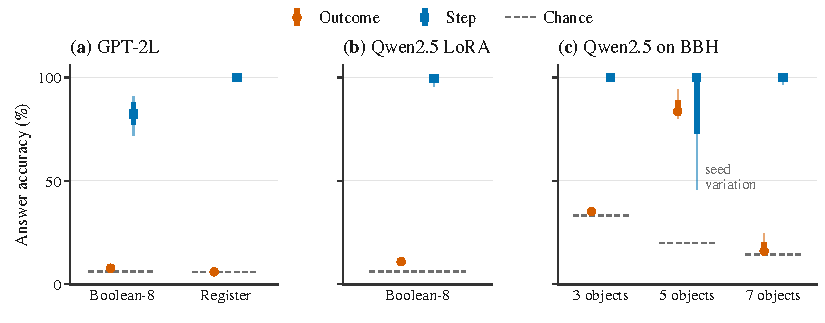
\includegraphics[width=\linewidth]{figures/main_transfer.pdf}
\caption{\textbf{Step supervision also helps beyond counting.}
Held-out answer accuracy for (a)~GPT-2L, (b)~Qwen2.5-0.5B LoRA, and (c)~Qwen2.5-0.5B LoRA on the official $250$ BIG-Bench Hard items at each object count.
Points show medians, thick intervals the interquartile range, and thin intervals the full seed range; GPT-2L Boolean-8 uses five seeds, other groups three.
Dashed segments show chance; exact values and protocols are in \cref{tab:main,app:experiments}.}
\label{fig:transfer}
\end{figure}
\paragraph{Purpose.} Synthetic state-tracking tasks test how degree structure relates to the supervision gap;
pretrained models and BIG-Bench Hard test whether the qualitative pattern transfers to a different setting.

\paragraph{Synthetic state tracking.} Boolean-8 has $4$ bits ($K=16$) and NOT, CNOT, SWAP and Toffoli gates on random wires ($n=8$); the register
machine has $(x,y)\in\mathbb Z_{17}^2$, five instructions, $n=16$ and answer $x$. Their answers put $98.9\%$ and $99.9\%$ of their
variance at degrees $\ge2$, while first occurrence keeps a degree-$1$ part at every $n$ (there $\mathbf 1[y=1]=b_1$, so $\E\|(\bm y-\bm u)_{\{1\}}\|^2\ge p(1-p)$). GPT-2L uses character tokens. \paragraph{Pretrained models and BIG-Bench Hard.} The LoRA runs test transfer of the qualitative mechanism beyond the controlled model.
On Boolean-8, giving Qwen2.5 eight times the outcome budget yields $10.0\pm0.9\%$ accuracy (mean$\pm$SD over seeds).
Answer-first controls give $8.0\pm0.9\%$ for GPT-2L and $10.1\pm1.0\%$ for Qwen2.5, so they do not reproduce the step benefit.



\noindent\begin{minipage}{\linewidth}
\emph{Benchmark setup and results.} Training items come from the benchmark's templates with new assignments and swaps; testing uses
the official $250$ items per size, all of which parse and rebuild exactly. Traces list every holder's item with its
option letter (``Alice has Ulysses (A)''); with item names alone, answers stayed at the letter base rate. With $m$
objects a random swap gives $\mixrate=\frac{mp-1}{m-1}$ with $p=\frac{\binom{m-1}{2}}{\binom{m}{2}}$, which is $0$, $\tfrac{1}{2}$ and $\tfrac{2}{3}$ for $m=3,5,7$, and the
share of answer variance at degrees $\le1$ is $\mixrate^{2n}+n\mixrate^{2(n-1)}(1-\mixrate^2)$: $0$, $1.56\%$ and $3.34\%$. Zero-shot accuracy is
$33.6$, $16.4$ and $11.2\%$. At three objects, outcome runs select the most common option, whose base rate is $35.2\%$.
Five objects reverse the ordering that the low-degree share predicts: outcome training reaches $80$--$94\%$ there but
$15$--$24\%$ at seven objects, whose share is larger. One of three five-object step runs fails ($46\%$ on real items, $45\%$ on
generated ones). Five objects are therefore an exception: outcome training succeeds despite less low-degree variance than seven objects.
We treat the degree calculation as a mechanistic guide, not a complete predictor of pretrained-model optimization; these LoRA runs are outside the theorem assumptions.
\end{minipage}





%=============================================================================

For the BBH spectrum measurement, we split all $6^3$ swap sequences at fixed scene, assignment and query, using the three option
logits and the LoRA up-projection Jacobian. For every task in \cref{tab:main}, $\mixrate$ is the largest singular value of the averaged
move permutation on mean-zero state vectors (\cref{def:lambda} for counting).
It determines the low-degree share for counting and BBH. For Boolean-8 and the register machine, it is only the slowest of many state modes:
the single-mode estimate $\mixrate^{2n}+n\mixrate^{2(n-1)}(1-\mixrate^2)$ gives $20\%$ and $56\%$, far above the measured
$1.1\%$ and $0.08\%$ degree-$\le1$ shares.

The summary counting rows use a zero readout and ten paired seeds with $8$k updates for modulo $2$ (mean accuracy, solved seeds in parentheses),
and $32$k updates with seeds $42$--$44$ for modulo $3$. BBH rows test on the $750$ official items, $250$ per size.

\begin{table}[H]
\centering\small
\fitwidth{\begin{tabular}{@{}llccccc@{}}
\toprule
Task & Model & $n$ & $\mixrate$ & outcome & step & chance\\
\midrule
count mod $2$ & two-block & $16$ & $0.50$ & $49.8$ ($0/10$) & $93.1$ ($8/10$) & $50$\\
count mod $3$ & two-block & $16$ & $0.66$ & $30$--$50$ & $100$ & $33$\\
first occurrence (control) & two-block & $8$--$24$ & -- & $71$--$100$ & $80$--$99$ & --\\
Boolean-8 & GPT-2L & $8$ & $0.82$ & $7.7$ & $82$ & $6.25$\\
register machine & GPT-2L & $16$ & $0.95$ & $6.3$ & $99.9$ & $5.9$\\
Boolean-8 & Qwen2.5-0.5B LoRA & $8$ & $0.82$ & $11.1$ & $98.3$ & $6.25$\\
\midrule
BBH, $3$ objects & Qwen2.5-0.5B LoRA & $3$ & $0$ & $35.2$ & $98.4$--$100$ & $33$\\
BBH, $5$ objects & Qwen2.5-0.5B LoRA & $5$ & $0.50$ & $80.0$--$94.4$ & $46$--$100$ & $20$\\
BBH, $7$ objects & Qwen2.5-0.5B LoRA & $7$ & $0.67$ & $15.2$--$24.4$ & $96.4$--$100$ & $14$\\
\bottomrule
\end{tabular}}
\caption{\textbf{Step supervision usually helps when the answer has little low-degree signal.}
Held-out accuracy (\%); ranges are over seeds. Detailed protocols and per-seed values are in the accompanying code repository.}
\label{tab:main}
\end{table}

%=============================================================================
\subsection{Joint routing runs}
\label{app:reach}

\Cref{tab:reach} uses the following protocol.
\begin{center}\small
\fitwidth{\begin{tabular}{@{}ll@{}}
\toprule
Model & two-block executor architecture (\cref{app:model}) \\
Task & counting modulo $2$, four letters, $p=\tfrac{1}{4}$ \\
Initialization & fan-in-scaled Gaussian weights, embeddings of variance $\frac{1}{d_{\mathrm{res}}}$, MLP biases of magnitude $1$--$2$,\\
& all scaled by $\initscale=0.3$; relative biases and readout zero\\
Trained & query/key maps, relative biases, readout (embeddings, values, MLPs fixed)\\
Optimizer & full-batch gradient descent, step size $2$, $4{,}096$ training prompts\\
Success & every state prediction on $16{,}384$ held-out prompts has positive margin\\
\bottomrule
\end{tabular}}
\end{center}
Of $17$ runs, $16$ solve; the remaining $n=12$ run reaches $99.95\%$ by $300$k updates. The outcome baseline uses the same
initialization, trained parameter subset, step size and data, with only the final count supervised; no outcome run
solves within $300$k updates. Implementation and per-run measurements are available in the accompanying code repository.

%=============================================================================
\section{Reproducibility}
\label{app:reproducibility}

% TODO before submission: confirm the anonymous repository URL.
\paragraph{Code.} Code, configurations, seeds, reproduction commands, numerical proof checks and per-run measurements are available at
\url{https://anonymous.4open.science/r/trace}. The accompanying code repository provides an exact implementation of the executors,
numerical checks of the reduced flow of \cref{thm:joint}(i) and the identities and constants of its clean-routing extension, and instructions for reproducing every experiment.

\paragraph{Compute and data.} Runs use one NVIDIA A100 80GB GPU: about one minute per $8$k counting updates and fifteen minutes per
$800$-update LoRA run; exploratory runs used more compute than reported. Data are synthetic; the accompanying code repository also
contains the official BIG-Bench Hard items, unchanged. Software and assets: PyTorch 2.13 (BSD-3-Clause), Transformers 5.16 and PEFT 0.20 (Apache-2.0), Qwen2.5-0.5B \citep{qwen2025qwen25} (Apache-2.0), and BIG-Bench Hard \citep{suzgun2022challenging} (MIT).

